\documentclass[12pt,oneside]{book}
\pagestyle{headings}

% Note that the line below could be modified to suit a
% particular system since the "geometry" package behaves
% differently in Unix, Windows and Mac, especially for the
% top margins.
% Adjust the parameter "top" (measuring the height of the 
% space allocated to a header) and "headsep" (measuring
% the distance from the bottom of the header to the
% first line of text.
\usepackage[top=1.3in,left=1.5in,bottom=1in,right=1in,headsep=0.5in]{geometry}

\usepackage{setspace}
\onehalfspacing
%\doublespacing

% Headers and footers for thesis
\usepackage{fancyhdr}

\markboth{}{}
\newcommand\startchapter[1]{\chapter{#1}\thispagestyle{myheadings}}
\newcommand\startappendix[1]{\chapter{#1}\thispagestyle{myheadings}}
\newcommand\startfirstchapter[1]{\chapter{#1}}

% Manual addition of section to Table of Contents
\newcommand\TOCadd[1]{\newpage\phantomsection\addcontentsline{toc}{chapter}{#1}}

% Float Customization
\renewcommand{\floatpagefraction}{0.01}

% Customization of Tables of Contents and List of Figures/Tables
\usepackage{tocloft}
\renewcommand\cfttabpresnum{Table\ }
\renewcommand\cfttabnumwidth{0.75in}
\renewcommand\cftfigpresnum{Figure\ }
\renewcommand\cftfignumwidth{0.80in}


% Long Table and decimal aligned columns
\usepackage{dcolumn}
\usepackage{longtable}

% Mathematics support
\usepackage{amsmath}
\usepackage{amsthm}
\usepackage{amssymb}


% Text Control
\usepackage{xspace}
\usepackage{textcase}

% Graphics
\usepackage{wasysym}
\usepackage{graphics}
\usepackage{graphicx}   % A package to allow insertion of
                        % external image files


\usepackage{url} 
\usepackage{hhline}
\usepackage{pdfpages}
\usepackage{multirow}
\usepackage{tabularx}
\usepackage{changepage}

\usepackage{array}
%\usepackage{makecell}
\newcolumntype{x}[1]{>{\centering\arraybackslash}p{#1}}

\usepackage{tikz}
\newcommand\diag[4]{%
  \multicolumn{1}{p{#2}|}{\hskip-\tabcolsep
    $\vcenter{\begin{tikzpicture}[baseline=0,anchor=south west,inner sep=#1]
        \path[use as bounding box] (0,0) rectangle (#2+2\tabcolsep,\baselineskip);
        \node[minimum width={#2+2\tabcolsep},minimum height=\baselineskip+\extrarowheight] (box) {};
        \draw (box.south west) -- (box.north east);
    \end{tikzpicture}}$\hskip-\tabcolsep}}

\begin{document}

% Front Matter
\input frontmatter/fm

\newpage

%%%%%%%%%%%%%%%%%%%%%%%%%%%%%%%%%%%%%%%%%%%%%%%%%%%%%%%%%%%%%%%%%%%%%%%%%%%%%%%%
%%%%%%%%%%%%%%%%%%%%%%%%%%%%%%%%%%%%%%%%%%%%%%%%%%%%%%%%%%%%%%%%%%%%%%%%%%%%%%%%
%% Chapter - Introduction
%%%%%%%%%%%%%%%%%%%%%%%%%%%%%%%%%%%%%%%%%%%%%%%%%%%%%%%%%%%%%%%%%%%%%%%%%%%%%%%%
%%%%%%%%%%%%%%%%%%%%%%%%%%%%%%%%%%%%%%%%%%%%%%%%%%%%%%%%%%%%%%%%%%%%%%%%%%%%%%%%

\startfirstchapter{Introduction}
\label{chap:introduction}

Feedback tools have been attracting great attention in recent years as sensing technology has become cheaper and more accessible. A large variety of tools have been designed and developed to assist people to collect data about themselves.  Computing technology has never been so available to everyone, irregardless of who is and who is \textit{not} an expert.  Designs of the user interfaces of feedback applications have been primarily devoted to coerce users into behavior change, some examples are to encourage them to take responsible energy behaviors at home, to exercise more, to practice breathing and meditation and many others.  With these tools and applications, people could know themselves better, be more informed about behavior choices and to take more control of their lives.  However, on deeper inspection, these applications are not as perfect as expected.  Behavior change does not necessarily result in the understanding of the cause and impact of behavior choices.  In many cases, people may take the suggestion to change their behavior even without understanding the behavior itself \cite{hand_explaining_2005,kuznetsov_upstream:_2010}.  The lack of context for reflection has been reported as one of the major barriers for personal information systems  (Chapter \ref{chap:pva}).  For example, evidence from a recent study \cite{neustaedter_everyday_2013} has shown that it is very difficult for people to link their daily routines to their residential energy consumption.
Meanwhile, feedback design also has to face the problem of low usage after passing the curiosity phase \cite{erickson_dubuque_2013}.  It is not uncommon that people keep trying out new applications only to stop using them after losing interest in them.  A lack of time was reported as one of the substantial barriers of ongoing adoption for personal informatics tools \cite{li_stage-based_2010}.  Temporal drop-offs in use are quite common to feedback systems \cite{bartram_design_2015,karapanos_user_2009, barreto_why_2013, ahtinen_user_2009, pierce_consideration_2010}.
The challenge is how to support the interpretation and development of knowledge and insight into behaviors and the causes behind them, while meanwhile facilitating the easy access to data within a context that requires minimal learning and management cost, to the goal of sustaining ongoing use of the tool.

With respect to this challenge, the questions are how to provide context in designs to help people understand their personal data and how to incorporate design components to encourage ongoing use of feedback applications.  First, designs should make the information fit naturally into peoples life patterns, leveraging their current information use habits.  Second the tools need to provide sufficient contextual information to help people understand not only the data patterns but also their causes. Finally, the effort required to gather and to integrate the various streams of data should be minimized: simply adding ``yet another app'' defeats this goal. 

Towards this end, I propose to integrate visualization of personal data (specifically in this thesis, data about household energy use and personal fitness) into a persons existing information eco-system, combining this with common information tools that represent the desired context (specifically in this thesis, personal digital calendars). Thus, \textit{the goal of the thesis is to investigate  
if the mash-up approach, integrating visualization of personal data on a digital calendar, is a viable design approach that is comprehensible and does not interfere people's existing information use habits (that is, regular calendar use),
how people interpret personal data within the context provided by their calendars,
and how people react and use the on-calendar visualizations in the field as a feedback tool.}
That is, this goal is not to develop novel visualizations per se, but rather to augment what people already use, thereby leveraging familiarity, reducing the overhead of using a separate application, and encouraging frequent observations of the data and ongoing use of feedback applications.

%role of feedback
In this thesis, the work focuses on applying the on-calendar visualization in feedback applications, specifically feedback for personal fitness and household energy conservation.  It is important to note that this type of data is common in people's lives, and understanding these data is important for individuals.  These tools can provide ongoing feedback of one's behaviors.  Better understanding of these patterns can help individuals make better behavior choices to influence their lives.  Visualization of this feedback data typically focus on answering three types of questions: \textit{what} (``what is the current status or progress''), \textit{why} (``why are the data patterns like this'', ``why did an anomaly happen''), and \textit{how} (``how could I improve'').  Self-realization and self-improvement depend on first understanding what has happened in the past, then reasoning about why the past data is the way it is, and finally using that insight to identify realistic changes that can make a difference.  The commonly used persuasive design strategy in this field usually focuses on \textit{how}, promoting action in the moment.  In contrast, my interest is to investigate how visualization design could enhance the reflective understanding of one's behaviors in a non-persuasive way. The general philosophy centers around helping people know their behavior with operational understanding \cite{bartram_design_2015} rather than digitally lecturing them into behavior change.  In this work, I view understanding as a first (but not the only) step towards encouraging new habits; therefore, tools that can succeed at this step have made progress.

Meanwhile, ongoing adoption is a commonly encountered barrier in personal information systems, especially in feedback designs, see chapter \ref{chap:pva}.  People have lower usage of the feedback tools although there is a high percentage of people who own at least one feedback tool.  Studies showed that people need to feel control of using their tools, and that this impact needs to be recognized by oneself or others \cite{ahtinen_user_2009}.  Adoption implies multiple phases in ongoing use.  Kim\cite{kim_inair:_2010} identified two stages of how people adopt everyday technologies: in the early stage, interest is the main motivation; then gradually the tool is adopted into daily routines. In a later stage, people's practices with the tool become ``rational reasoning rather than from an unconscious and habitual reiteration''; that is, using the tool becomes part of their routines. People's goals are mostly realized in the latter stage; however, the transition to this stage takes time.  Whether the transition occurs at all depends on how easily the tool fits into the person's life.

%%% calendars
Calendars are both a planning tool and a record of people's daily activities, and thus may be useful in helping people understand data that are related to activities and locations (such as resource use, medical tracking, calorie counting, or spending).
Calendar views have several advantages: the timeline aligns with the temporal data, time can be adjusted into different time scales to provide an overview and details as needed, and calendars represent the periodic nature of time-based data \cite{van_wijk_cluster_1999}.  The use of a digital calendar is a common practice nowadays. The familiarity of calendar views and the routine use of calendars should require low learning and management cost, and should easily fit into one's life routines.  More importantly, calendar events provide rich contextual information about one's daily life, which could be relevant to understanding personal data.  Evidence shows that people are inclined to check personal calendars for reasoning about purpose in everyday life \cite{baur_streams_2010,lee_reflecting_2011,mcduff_affectaura:_2012,neustaedter_everyday_2013}.  Thus, a personal digital calendar can provide appropriate contextual framing in helping people recognize and understand information patterns.

%design requirement or challenges (specific)
However, the display of additional visualization layers on a calendar needs to be approached with care.  When we ``mash-up'' information sources in a familiar tool, we need to ensure that the additional information is attentionally ambient to avoid interfering with the primary function of the application (digital calendar tasks in this case).  Thus when adding data to an information space that may already be dense (the calendar), the visualization design has to balance visual interference with normal calendar tasks, and attention should be placed on the perceptability and legibility of the added data stream.  The design needs to minimize visual interference while supporting effective data perception.  Meanwhile, reasoning about personal data and developing self knowledge is a long-term process, and using feedback tools in everyday life is quite different, compared with using visualization tools in an occupational situation \ref{chap:}.  Especially, investigating how people use the feedback tool and reason about the data with the on-calendar visualization requires a real life context. 

%Particularly, I am interested in how people reason about their data with the context provided by personal calendars and

%overview of the studies
Thus, the study is divided in multiple phases: a systematic literature review, a viability study to confirm the design goal and narrow down design alternatives, case studies to test the design concept and the implemented prototype, and a longitudinal field study to deeply investigate how the on-calendar feedback tool is used in everyday life context.  First, I reviewed the literatures of visualization designs used in everyday life to identify design dimensions and challenges in personal visualization.  I proposed the design approach and alternatives, and aimed to tackle two challenges in literature: providing contextual information to enhance understanding and easy access to encourage on-going use.
After that, I conducted a lab study to evaluate design alternatives with respect to the interference and the perceptability.  With the selected visualization alternatives based on the study results, I implemented an on-calendar visualization linked Google Calendar with live personal data streams (from residence smart meter and Fitbit devices, respectively). The implementation was later improved based on two case studies: household electricity conservation and personal fitness. Finally, I deployed it as a fitness feedback tool in an eight-week field study, investigating how people interact with the on-calendar design and how they use context to reason about their Fibit data in the field. 

%research questions
These studies are designed to answer the following research questions:
\begin{itemize}
	\item{Shat are the current challenges in designing visualization used in everyday life}
	\item{Are the on-calendar visualization comprehensible and do not interfere with primary calendar tasks?}
	\item{What are the design options that can balance the interference and perceptability for the on-calendar visualization?}
	\item{To what extent can people use calendar events as context for reasoning about their personal data?}
	\item{Could people improve their understanding of their data and behaviors better with the context provided by personal digital calendars?}
	\item{How do people react and use the on-calendar visualization as the feedback tool in everyday life?}
	\item{Is the mash-up feedback tool easy to learn and manage in everyday life?}
\end{itemize}


This thesis describes the following significant and novel contributions:
\begin{enumerate}
\item The first systematic literature review of Personal Visualization and Personal Visual Analytics.  It provides the starting point for researchers and designers to re-think about new design requirements and design dimensions for applying visualization design in everyday life context.  This work brings together research that was previously scattered in different disciplines and research fields.

\item A design approach that integrates the visualization of personal data (personal fitness and home energy consumption) into people's existing information eco-system (a personal digital calendar).  It can provide daily-life context for people to better understand their fitness data and home energy use.  This approach incorporates people's existing habit of information use, requiring low learning and managing cost and engaging ongoing use.

\item A definition for \textit{attentional ambience}, extending ambient visualization from spatial location (displayed in peripheral location) to attentional demand, with which ambient visualization can be centrally located as an additional visual layer and where the perception transiting between foreground and background depends on the degree of attention. This perspective changes ``environmentally appropriate'' to ``attentionally appropriate'' with respect to attentional demand.

\item Quantitative lab experiments to evaluate visual interference and perceptability of design alternatives of on-calendar visualization.  These experiments showed the promise of the proposed mash-up approach where additional visualization layers could be perceived ambiently with proper visualization choices.

\item Qualitative field deployments to investigate how people react to the mash-up approach and use contextual information from personal calendars to reason about personal data in real life context. The studies confirmed that personal digital calendars could provide rich contextual information for people to reason about their data. Particularly, they proved helpful in identification and reasoning about data patterns and anomalies.  In addition, the on-calendar visualization made the relevant information easy to access.

\item A new feedback model of design components in feedback designs based on the study results.  The model offers a structure to investigate the connection of design components in feedback design, and also indicates possible evaluation dimensions of feedback tools.  It provides a starting point for thinking about how design characteristics might influence feedback tool use, including the likelihood of ongoing adoption and behavior change.
  
\end{enumerate}

%extend application
Although this work focuses on feedback scenarios, the on-calendar visualizations could be applied to many other types of data, at either individual or organization levels. For example, individuals might monitor physical activity, ratings of mood, or physiological indicators such as heart rate.  Organizations might visualize network traffic or density of people present in a facility, and relate these to group activities or public events. Thus our investigation of on-calendar visualizations provides a foundation for exploring a potentially large design space of attentionally ambient visualizations.

In the following chapters of this thesis, a systematical review across several fields is devoted first to identify design unique requirements, design dimensions and challenges of personal visualization \& personal visual analytics (PV\&PVA) used in everyday life in Chapter \ref{chap:pva}.  Among all the challenges, this work focuses on how to provide context for people to reason about personal data and how to make it easily fit into everyday life routines.  A review of related work from the literature is presented next in Chapter \ref{chap:relatedWork}, in which I discuss examples of feedback design and the commonly used design strategies - persuasive design and ambient design, together with evaluation methods in visualization design and Human Computer Interaction (HCI).  I propose the design approach and the visualization alternatives in Chapter \ref{chap:visdesign} based on visualization design principles.  After that, I summarize the the research method in this thesis to investigate the on-calendar design approach (in Chapter \ref{chap:design}). First, a viability study was used to evaluate the design alternatives with respect to visual interference and perceptability, in Chapter \ref{chap:viability study}.  As the design concept was confirmed in the viability study, a working prototype (a web based application) was implemented with selected design alternatives from the viability study (in Chapter \ref{chap:implementaiton}).  To test the early version of implementation in real life context, I deployed the application in two case studies (home energy conservation and personal fitness) as pilot studies (Chapter \ref{chap:pilot studies}), where the application was connected with real time data (household smart meter and Fitbit devices respectively) and participants' Google Calendar.  After the revised version of on-calendar visualization was implemented, I deployed it in an eight-week field study (in Chapter \ref{chap:field study}), aiming to investigate how people react to the integration approach and how they reason about their data with contextual information from personal calendars in everyday life. Some future work are then presented in Chapter \ref{chap:future work}, along with conclusion in Chapter \ref{chap:conclusion}.

(appendix) edit this part in the end
******************************
Supplementary information including a list of ...
%After that a chapter devoted to a review
%of the audio feature extraction and machine learning algorithms in
%Chapter \ref{chap:analysis} ``Automatic and Semi-Automatic Analysis''.  

%Datasets obtained with the use of this Orchive system will be then
%used as input on these audio feature extraction and machine learning
%algorithms and results will be presented in Chapter
%\ref{chap:evaluation}.  Results from the citizen science experiment
%will be presented in chapter \ref{chap:citizenscienceevaluation}, and
%a chapter discussing the results from experts users will be presented
%in Chapter \ref{chap:expertinterfaceevaluation}.  Conclusions will
%then be presented along with Future Work in Chapter
%\ref{chap:conclusions}.  Supplementary information including a list of
%the web resources developed in this thesis in Appendix
%\ref{chap:weblinks}, Glossary in Appendix \ref{chap:glossary},
%Bibliography and Publications from this Research in Appendix
%\ref{chap:publications} will be followed by Appendix \ref{chap:ABMI}
%about our ongoing collaboration with the Alberta Biodiversity
%Monitoring Institute, to use this software to help estimate bird
%biodiversity.


****************************

%%%%%%%%%%%%%%%%%%%%%%%%%%%%%%%%%%%%%%%%%%%%%%%%%%%%%%%%%%%%%%%%%%%%%%%%%%%%%%%%
%%%%%%%%%%%%%%%%%%%%%%%%%%%%%%%%%%%%%%%%%%%%%%%%%%%%%%%%%%%%%%%%%%%%%%%%%%%%%%%%
%% Chapter - PVA
%%%%%%%%%%%%%%%%%%%%%%%%%%%%%%%%%%%%%%%%%%%%%%%%%%%%%%%%%%%%%%%%%%%%%%%%%%%%%%%%
%%%%%%%%%%%%%%%%%%%%%%%%%%%%%%%%%%%%%%%%%%%%%%%%%%%%%%%%%%%%%%%%%%%%%%%%%%%%%%%%

\startchapter{Personal Visualization and Personal Visual Analytics}
\label{chap:pva}
%intro: motivation, contribution
Visualizing personally interested or related data have attracted a great amount of attention in recently research and practice.  However, pieces of this type of work scatter in several research communities, for example, environmental psychology, personal informatics, ambient visualization, information visualization and human computer interaction.  There was no work before that provides systematic review of visualization work and no work to bridge this research among these communities.  Meanwhile, gaining knowledge of the design patterns and gaps in previous practice should be the first step in a study and should precede the design phase.  Thus, a literature review of existing personal visualization and personal visual analytics work is necessary to identify design dimensions and challenges in this field. 

In the following section I start with the overview of current research in this field.  I then describe the review method and process.  After summarizing the current design dimensions and patterns, I discuss the challenges the future research needs to face.

\section{Background}

We are surrounded by data in our everyday lives. Data relevant to our personal lives are increasingly available, often due to advances that make data easier to access or collect.  These data cross a broad spectrum of domains and scope.  For instance, due to Open Access policies, we now have immense data stores about our communities (e.g. census data); due to commercial availability of sensors, our health and fitness (e.g. exercise logs, pedometer data), and even data on our resource usage (e.g. utilities, such as water, energy use) data is easily available to us.  Some of this data collection is done without our explicit attention: our mobile devices, for instance, track our use of digital and social media to organize, plan, and connect with others; similarly, our web browsers collect digital traces of our online activities.  Increasingly though, we are going out of our way to collect about ourselves (e.g.,the ``Quantified self'' movement).  These data are relevant to our personal lives - they enable us to explore information about ourselves, our communities, and issues that are personally relevant and important to us.  As the volume of data grows substantially, exploring and analyzing these data becomes a common daily demand, especially for people who are not data experts in their lives. 

%A well-know example is the ``Quantified self'' movement,where people design tools to collect and understand personal data. However, the problem people need to face nowadays is not the lack of data, but data overwhiming. Acquiring data does not automatically come into insights that people can process cognitively.

% One example is the life logging \cite{allen_dredging_2008,sellen_life-logging_2007}, where people use sensoring and tracking technology to record personal archives together with environmental measures. However, it does not really have a practical purpose and fails its expectation \cite{sellen_beyond_2010}. Study also showed people barely re-visit thier data archives after they were collected \cite{petrelli_family_2010,whittaker_easy_2010}.  

The value of data comes only after transforming data into insights.  Visualization is a powerful practice in this transformation.  However, research into this practice has been mostly focused on professional situations.  As the interest of applying visualization in everyday life to explore personal data or personal relevant data is growing, how can we better design visualizations to meet this fast growing need?  What are the new requirements and challenges researchers and designers have to face?
Since the relevant research is currently scattered in several communities, to establish a common language of such visualization design I describe previous and future work as being part of a new field and research community called personal visualization and personal visual analytics.

\textit{Personal Visualization (PV) involves the design of interactive
visual data representations for use in a personal context, and Personal Visual Analytics (PVA) is the science of analytical reasoning facilitated by visual representations used within a personal context.} 

The main question that PV\&PVA is concerned with is:  How can the power of visualization and visual analytics be made appropriate for use in personal contexts - including those for people who have little experience with data, visualization, or statistical reasoning?  There is enormous potential for us to use data to make positive changes in our personal lives and the lives of others, but as visualization and visual analytics experts are well aware, greater availability of data does not on its own lead to new insights.  Data must be accessible, understandable, and interpretable before interacting with it can lead to insights or actionable knowledge.  Adoption of PV\&PVA technologies also depends on how well those technologies fit into people's daily environments and routines.  PV\&PVA builds on work in visualization (Vis) and visual analytics (VA) and aims to empower everyday users to develop insights within a personal context.  Personal context implies non-professional situations, in which people may have quite different motivations, priorities, role expectations, environments, or time and resource budgets as compared to professional situations.  Because of these differences, PV\&PVA designs necessarily have new requirements and challenges that bring new opportunities for Vis and VA research.

I reviewed existing PV\&PVA literature across several fields to identify common approaches, findings and gaps.  This work helps to establish an initial set of design dimensions to characterize this space and provide a common vocabulary that will make it easier to relate and share information between fields, which offers a starting point to learn about the challenges that arise when designing for personal contexts.

\section{Review Method and Process}
In this section, I describe the review method and process, with which a set of design dimensions characterizing the design space of PV\&PVA research was articulated. These dimensions relate to data, context, interaction and insights (in Table \ref{dimension}).  These dimensions provides a common ground to identify clusters of work and also challenges in this area.

As part of our iterative process, I conducted an extensive literature survey of PV\&PV A designs.  First, I systematically identified relevant papers from TVCG (including VIS papers), CHI papers and notes, UBICOMP, INTERACT, AVI, EuroVis, and PacificVis from 2008-2012, plus CHI 2013 since those papers were available at the time.  Relevance was based on meeting all of the following criteria:

\begin{itemize}
	\item{Data were about oneself, one's family or community, or relevant to personal interest or needs.}
	\item{Designs were intended to help people develop insights within a personal context (system design goal). Visualizations designed to support occupational roles or tasks were excluded (e.g., those specifically designed for domain experts or analysts in an occupational role).}
	\item{Designers intended the visualizations to be viewed from a non-professional perspective (e.g., from a self-centered viewpoint). Visualizations intended for use from an analyst's perspective or that required professional training were excluded.}
	\item{Research focused on visualization and interaction design or their evaluation. Papers that focused on system architecture, system optimization or algorithms were excluded.}
\end{itemize}

This resulted in a set of 59 papers that was complemented with a list with an additional seven papers encountered in other domain specific venues (summary in Table \ref{table:dimension}).
The development of the taxonomy of PV\&PV A design dimensions was based on an iterative, bottom-up approach.  The objective was to identify and articulate a set of dimensions that could adequately describe and distinguish among PV\&PVA tools in the literature.  The dimensions evolved much like a process of open coding, where a set of dimensions and levels was iteratively mapped and adjusted with the literature.  I considered this set of dimensions and levels to be complete when the collaborators reached consensus and could adequately represent the unique attributes of PV\&PVA tools in the collection. The final set of dimensions are in Table \ref{table:dimension}.


\begin{table}[]
\begin{center}
\caption{Design dimensions, levels with examples from the literature}
\begin{adjustwidth}{-1.1in}{} 
\resizebox{7.8in}{!}{\begin{tabular}{|l|l|l|l|l|}
\hline
Categories                & Dimensions                                                                 & Definition                                                                                                                                                      & Levels          & Examples                                                                                                                                                                 \\ \hline
\multirow{11}{*}{Data}    & \multirow{4}{*}{Data Scope}                                                & \multirow{4}{*}{Who the data is about}                                                                                                                          & self            & Sleep quality {[}7{]}                                                                                                                                                    \\ \cline{4-5} 
                          &                                                                            &                                                                                                                                                                 & family          & Internet bandwidth shared at home {[}14{]}                                                                                                                               \\ \cline{4-5} 
                          &                                                                            &                                                                                                                                                                 & peers           & Relationship with friends {[}37{]}                                                                                                                                       \\ \cline{4-5} 
                          &                                                                            &                                                                                                                                                                 & community       & Hang-out patterns on campus {[}75{]}, online conversations{[}29{]}                                                                                                       \\ \cline{2-5} 
                          & \multirow{4}{*}{Data Effort}                                               & \multirow{4}{*}{\begin{tabular}[c]{@{}l@{}}Amount of effort that is \\ expended in data collection\end{tabular}}                                                & none            & Online search history {[}6{]}                                                                                                                                            \\ \cline{4-5} 
                          &                                                                            &                                                                                                                                                                 & sensor          & Nonobtrusive sensing devices, e.g, wearable sensors {[}31{]}                                                                                                             \\ \cline{4-5} 
                          &                                                                            &                                                                                                                                                                 & manual          & Manual logging pictures and annotations {[}62{]}                                                                                                                         \\ \cline{4-5} 
                          &                                                                            &                                                                                                                                                                 & mixed           & Combination of sensor recording and manual input {[}58{]}                                                                                                                \\ \cline{2-5} 
                          & \multirow{3}{*}{Data Agency}                                               & \multirow{3}{*}{\begin{tabular}[c]{@{}l@{}}The degree of control a person has \\ over what data is collected, and when\\  and how it is collected\end{tabular}} & no control      & Online conversation logs {[}29{]}                                                                                                                                        \\ \cline{4-5} 
                          &                                                                            &                                                                                                                                                                 & partial control & \begin{tabular}[c]{@{}l@{}}Users have control of whether or not to collect the data, but \\ cannot customize what data they would like to collect {[}31{]}\end{tabular}  \\ \cline{4-5} 
                          &                                                                            &                                                                                                                                                                 & total control   & Manually recorded children’s photos and growth progress {[}45{]}                                                                                                         \\ \hline
\multirow{10}{*}{Context} & \multirow{4}{*}{\begin{tabular}[c]{@{}l@{}}Design \\ Context\end{tabular}} & \multirow{4}{*}{\begin{tabular}[c]{@{}l@{}}Who designed and \\ developed the  application\end{tabular}}                                                         & self            & Visualization designed by oneself                                                                                                                                        \\ \cline{4-5} 
                          &                                                                            &                                                                                                                                                                 & group           & Tools designed by a study group to chart their progress                                                                                                                  \\ \cline{4-5} 
                          &                                                                            &                                                                                                                                                                 & participatory   & \begin{tabular}[c]{@{}l@{}}Using an online survey to get feedback on early visual design \\ concepts {[}31{]}\end{tabular}                                               \\ \cline{4-5} 
                          &                                                                            &                                                                                                                                                                 & third party     & \begin{tabular}[c]{@{}l@{}}Visualization of music listening history designed by \\ the researcher {[}9{]}\end{tabular}                                                   \\ \cline{2-5} 
                          & \multirow{6}{*}{Settings}                                                  & \multirow{6}{*}{\begin{tabular}[c]{@{}l@{}}In what situation the tool is \\ used and how it is used\end{tabular}}                                               & personal        & Personal laptop (mostly non-mobile but used by oneself) {[}65{]}                                                                                                         \\ \cline{4-5} 
                          &                                                                            &                                                                                                                                                                 & domestic        & Ambient display at home (mostly non-mobile){[}32{]}                                                                                                                      \\ \cline{4-5} 
                          &                                                                            &                                                                                                                                                                 & mobile          & Used on a mobile phone while on-the-go {[}31{]}                                                                                                                          \\ \cline{4-5} 
                          &                                                                            &                                                                                                                                                                 & shared          & Visualization of physical activities viewed by co-workers {[}60{]}                                                                                                       \\ \cline{4-5} 
                          &                                                                            &                                                                                                                                                                 & public          & \begin{tabular}[c]{@{}l@{}}Visualization to promote energy conservation presented in \\ a public space {[}41{]}\end{tabular}                                             \\ \cline{4-5} 
                          &                                                                            &                                                                                                                                                                 & mixed           & \begin{tabular}[c]{@{}l@{}}Combination of above, e.g., visualization of residential energy \\ on a personal computer and a mobile phone {[}5{]}\end{tabular}             \\ \hline
\multirow{10}{*}{}        & \multirow{4}{*}{Influence Context}                                         & \multirow{4}{*}{\begin{tabular}[c]{@{}l@{}}Who the application is \\ intended to inform\end{tabular}}                                                           & self            & My physical condition {[}19{]}                                                                                                                                           \\ \cline{4-5} 
                          &                                                                            &                                                                                                                                                                 & family          & Children’s growth progress {[}45{]}                                                                                                                                      \\ \cline{4-5} 
                          &                                                                            &                                                                                                                                                                 & community       & Inform public about elections {[}84{]}                                                                                                                                   \\ \cline{4-5} 
                          &                                                                            &                                                                                                                                                                 & mixed           & Encourage water drinking for peers and oneself {[}16{]}                                                                                                                  \\ \cline{2-5} 
                          & \multirow{3}{*}{Attentional Demand}                                        & \multirow{3}{*}{\begin{tabular}[c]{@{}l@{}}How much attention is \\ required to interact \\ with the tool\end{tabular}}                                         & low             & Cell phone wall paper {[}7{]}, ambient display {[}32{]}                                                                                                                  \\ \cline{4-5} 
                          &                                                                            &                                                                                                                                                                 & mixed           & \begin{tabular}[c]{@{}l@{}}Pedometer counter on a cell phone and the historical data \\ on a desktop {[}58{]}\end{tabular}                                               \\ \cline{4-5} 
                          &                                                                            &                                                                                                                                                                 & high            & Exploration of music listening history with focused attention {[}9{]}                                                                                                    \\ \cline{2-5} 
                          & \multirow{3}{*}{Explorability}                                             & \multirow{3}{*}{\begin{tabular}[c]{@{}l@{}}The ability to explore \\ the data\end{tabular}}                                                                     & low             & Visual metaphor representing one’s physical activities {[}31{]}                                                                                                          \\ \cline{4-5} 
                          &                                                                            &                                                                                                                                                                 & mixed           & \begin{tabular}[c]{@{}l@{}}Data overview on a cell phone and exploration of history \\ data on a client service {[}5{]}\end{tabular}                                     \\ \cline{4-5} 
                          &                                                                            &                                                                                                                                                                 & high            & Exploring historical data with dynamic queries {[}9{]}                                                                                                                   \\ \hline
\multirow{4}{*}{Insight}  & \multirow{3}{*}{Actionability}                                             & \multirow{3}{*}{\begin{tabular}[c]{@{}l@{}}Degree to which the insight \\ gained from using the tool \\ can guide future actions\end{tabular}}                  & low             & \begin{tabular}[c]{@{}l@{}}Does not inform further action, e.g., supports reminiscing \\ about the past {[}68{]}\end{tabular}                                            \\ \cline{4-5} 
                          &                                                                            &                                                                                                                                                                 & mixed           & \begin{tabular}[c]{@{}l@{}}Smartphone app that gives reminders about when to exercise \\ and enables reflection on progress via historical records {[}58{]}\end{tabular} \\ \cline{4-5} 
                          &                                                                            &                                                                                                                                                                 & high            & \begin{tabular}[c]{@{}l@{}}Engages a certain behavior, e.g., encourage energy\\  conservation {[}50{]}\end{tabular}                                                      \\ \cline{2-5} 
                          & Automated Analysis                                                         & \begin{tabular}[c]{@{}l@{}}Data mining or other \\ automated analysis methods\\  are employed\end{tabular}                                                      & Yes/No          & Classify physical activities to types of transportation {[}31{]}                                                                                                         \\ \hline
\end{tabular}}
\label{table:dimension}
\end{adjustwidth}
\end{center}
\end{table}

To reduce redundancy while discussing the design dimensions (Table \ref{table:dimension}) when more than one paper was based on the same visualization tool this work refers only to their latest version of the tool. This reduced the set of 66 papers to 59 designs \ref{table:venu}.

\begin{table}[]
\centering
\begin{tabularx}{\textwidth}{|X|X|X|X|X|}
\hline 
            & \begin{tabular}[c]{@{}l@{}}VIS\\  Community\end{tabular} & \begin{tabular}[c]{@{}l@{}}HCI\\ Community\end{tabular} & Other & Total \\
Before 2008 &                             &        & 2     & 2     \\ \hline
2008        & 2                           & 6       & 1     & 9     \\ \hline
2009        & 1                           & 7      & 0     & 8     \\ \hline
2010        & 3                           & 6      & 3     & 12    \\ \hline
2011        & 2                           & 8      & 0     & 10    \\ \hline
2012        & 2                           & 16     & 1     & 19    \\ \hline
2013        &                    & 6    &      & 6     \\ \hline
Total       & 10                         & 49      & 7     & 66   
\\ \hline
\end{tabularx}
\caption{Summary of surveyed papers}
\label{table:venu}
\end{table}

\section{Design Dimensions and Research Interest to Date}
With the collection of 59 designs, I coded and mapped them to an interactive parallel plot of design dimensions that helped to identify design trends and research interest to date. The most prevalent characteristics of existing PV\&PVA tools can be observed by looking at the sizes of the boxes (representing levels within the dimensions) in Figure \ref{fig:rw_pva}. As exploring the interactive parallel plot, I articulate these dimensions in the design space and discuss the research interest to date in this section.

\begin{figure}[ht]
\centering
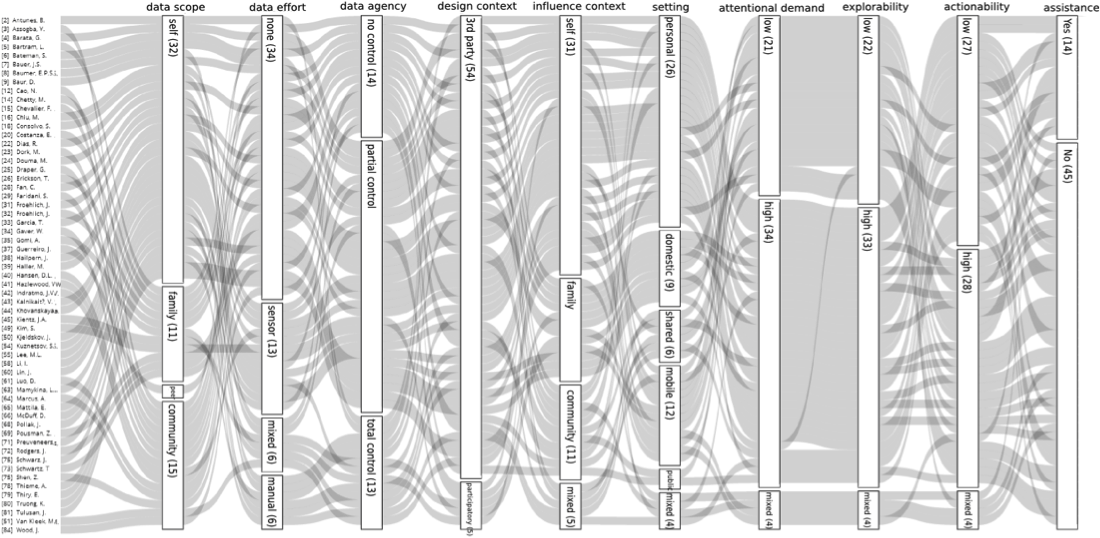
\includegraphics[width=\columnwidth]{figures/RW_pva}
\label{fig:rw_pva}
\caption{PV\&PVA design dimensions (parallel axes) and surveyed tools (first axis). Box sizes indicate the number of tools with each classification. Linked highlighting enables cluster exploration.}
\end{figure}

\subsection{Design Dimensions}
From a data effort level, the most common situation was that data were either provided, requiring no effort (e.g., by web servers or system logs) or non-intrusively collected by sensors (with partial personal control).  If data collection required no effort or people had little control over the data collection, the tools mostly had low actionability (34 out of 45 cases, seen by hovering the mouse over ``no effort'' or ``no control'' in the interactive visualization \ref{fig:rw_pva}). The literature showed that people could achieve total control over data collection (what, how and when to record) only when they manually recorded or organized data;  this occurred mostly in applications for personal health (9 out of 13 cases).  Much less control was provided if data were collected through public channels such as social networks. 

The practice of PV\&PVA are mediated within personal context. In activity theory, Nardi \cite{nardi_context_1995} argued that context is ``both internal, involving specific objects and goals and, at the same time, external to people, involving artifacts, other people, and specific settings''.  Internally, context could be ``abstract artifacts'' \cite{kaptelinin_acting_2009}, such as goals, skill sets, preferences, experience, etc.  Externally, context could be either physical constraints (e.g., physical environments or devices) or social influence (e.g., norms in a community or division of labor).  In a personal context, people may look into their own data with different goals, backgrounds, and expectations (i.e., internal context), which can highly influence how they interact with the designs and what information and insights they could get from data.  External factors that may characterize personal context include devices, use context and social influence.  From the literature, most of the tools were intended to develop insights for one's family or oneself.  We observed that nearly all PV\&PVA tools were designed by third parties (we reflect on this design perspective in section 6.5).  However, the literature suggests that involving participants in the design process (participatory design) might be related to higher actionability (all 5 participatory designs achieved high actionability).  Meanwhile, the tool set in our selection covers most use contexts: ambient displays at home, mobile devices on the go, personal computers or laptops used in a personal space, shared views with others, and displays for the public. It seems that applying the use of mobile devices and shared views aimed to achieve higher actionability (14 out of 16 cases).

PV\&PVA designs also covered a wide range of interactions, facilitating diverse attentional demands and explorability.  Many of the tools, mostly with mobile devices or ambient displays, did not require focused attention (25 out of 59 cases).

From an insight perspective, not all PV\&PVA designs were intended to reveal actionable knowledge (low actionability: 27 out of 59 cases).  People also used these tools to satisfy their curiosity (e.g., exploring census data), to reminisce about experiences, or to share with others (e.g., exploring activity traces at home).  Interestingly, although the use of automated computational assistance (e.g., classification algorithms) is common in visual analytics generally, this type of analysis was not common in the tools that we surveyed (14 out of 59 cases).  Examples included sentiment analysis and classification of physical activities.

\subsection{Research Interest to Date}
Reviewing the design collection and exploring the the parallel plot revealed the emerging interest in this field (what people have been working on) and possible gaps (i.e., research opportunities).  Note that the clusters were not meant to be mutually exclusive or systematically categorize the design space; instead, they illustrated interesting relationships between design dimensions and highlighted some research trends to date. 

\subsubsection{Attentional Demand (high), Explorability (high), and Actionability (mostly low)}
The first trend is designs for \textit{enabling exploration for curiosity} that requires high attentional demand and supported a high level of explorability. Insights obtained from using the tools were typically not very actionable, and were mostly used to understand something rather than to support taking specific actions or making changes.
Tools in this category were similar to traditional visualization tools, but usually had a self-centered focus (``my documents'' \cite{antunes_this_2009}, ``my computer usage'' \cite{barata_appinsight:_2012}, ``places I have been to'' \cite{kalnikaite_now_2010} or ``my finance'' \cite{schwarz_reflections_2009}).  These tools enabled user exploration facilitated by typical analytical tasks such as select, reconfigure, encode, elaborate, filter, connect, etc.  For example,  by interactively exploring (like as in traditional InfoVis techniques) with music listening history \cite{baur_streams_2010} people could investigate their listening patterns or re-experience a special life event in the past (as musical experiences are usually associated with events).  Interaction techniques for tools in this cluster supported exploration (high explorability) that may help people narratively develop stories from their data. This might be the first phase of adoption of these tools. 

For many tools in this cluster, personal knowledge and experience played an important role in the data interpretation process.  For example, whether or not someone listens to music on a particular date depends on daily routines and special events \cite{baur_streams_2010}.  Spending data can be explained by relevant routine activities, e.g., coffee drinking habits \cite{schwarz_reflections_2009}.  This implies that effectiveness of tools in this category could be dependent on highly personal factors. Yet most evaluations of tools in this cluster (12 out of 16) involved lab studies measuring task efficiency and error rate on experimentally controlled tasks with ``hard-coded'' use contexts. While such laboratory studies are common practice in VIS and VA research, they have limitations for evaluating PV\&PVA applications. 

\subsubsection{Attentional Demand (low), Explorability (low), and Actionability (mostly high)}
Another common design trend is to \textit{provide in-the-moment or on-going awareness with respect to personal behaviors}.
This practice was mostly applied in personal health or energy conservation, where they were expected to avoid interrupting life routines by combining low attentional demand and just-sufficient salience, for example, through a strategy of ambience (e.g., cell phone wallpaper).  For example, through cell phone wallpaper, ShutEye indicated sleep-related activity \cite{bauer_shuteye:_2012}. Interactions with tools in this cluster tended to be simple to fit in the on-the-go or ambient context and to efficiently provide key information as needed. 

Some tools in this cluster used machine learning or data mining algorithms to assist with data aggregation or disaggregation, e.g., classifying accelerometer data into physical activities \cite{consolvo_activity_2008} or disaggregating water consumption based on water use behaviors \cite{froehlich_design_2012}.  Some used graphical metaphors to remind people of the potential impact of their behavior. For example, to encourage people to exercise and to take green transportation \cite{froehlich_ubigreen:_2009}, a polar bear on a piece of ice was displayed; the ice began to melt if the user's behavior was not environmentally friendly.  This example also reveals the special PV\&PVA requirements in terms of aesthetics and emotional engagement.

Social influence was often used as a persuasive strategy to engage behavior change (e.g., for drinking more water \cite{chiu_playful_2009}, staying physically active \cite{lin_fishnsteps:_2006} or encouraging recycling \cite{thieme_weve_2012}).  However, social engagement and comparison may also raise other problems: inappropriate social strategies actually made the design less effective or caused undue stress \cite{thieme_weve_2012}, and the viewing of other people's personal data also raises privacy concerns.
 
\subsubsection{Data scope (family), influence context (family), and setting (domestic)}
Systems designed for families focused on \textit{data about family members or the home environment, and were used or deployed domestically}.
Some applications used decorative ambient displays to make the technology less intrusive and to better fit in the home environment \cite{froehlich_design_2012}; others ran on a personal computer, enabling close exploration and organization of family data to track progress \cite{kientz_baby_2009}.  These applications were designed to monitor or engage behaviors towards family health, energy conservation, domestic resource sharing, or social interaction of family members. 

In many cases, visualization designs consider individual differences among family members, for example, customizing views to adapt to difference cognitive levels (children v.s. adults) in the family \cite{froehlich_design_2012}. 
Additional contextual knowledge was also provided in visualizations to help people interpret the data, for example, by narratively depicting quantitative measures \cite{froehlich_design_2012}, which facilitate a better understanding of the family data.
Meanwhile, interaction and sharing within families can bring up issues of competition, cooperation and privacy. For example, a visualization of Internet traffic \cite{chetty_why_2011} was designed to educate family members about their shared Internet usage. Family members could view each other's online activities and bandwidth usage could be prioritized with respect to social roles. Here, some family members noted an unwelcome intrusion on privacy. The challenge is how to balance the diversity of users in a family, with respect to cognitive capabilities, skills, and social roles.

\subsubsection{Data scope (community), data effort (none), data agency (no control), and influence context (community)}
Beyond individuals and their families, research interest also revealed that people are also curious and care about the \textit{communities} they live in.
These designs were usually intended to inform the public or a certain social group, e.g., raising public awareness of elections \cite{wood_ballotmaps:_2011}, supporting easy exploration of survey data \cite{draper_who_2008}, or revealing topics evolving from social networks \cite{dork_visual_2010,faridani_opinion_2010}.  In a few examples, they were also used to encourage behaviors valued within the community, for example, ambient displays deployed in a department lobby to encourage energy conservation and physical activities\cite{hazlewood_issues_2011}.

Tools in this cluster mostly supported focused data exploration tasks, similar to other Vis and VA applications; they employed many traditional visualization techniques to facilitate deep analysis and usually required high attentional demand.  In several cases, automated computational analysis was used for mining large data sets from social networks (4 out of 11), e.g., peak-finding \cite{marcus_twitinfo:_2011} and sentiment analysis \cite{dork_visual_2010}.  Traditional Vis and VA techniques may work well to support reflection on community data.  However, since public data may not be too personally relevant, such tools may benefit from employing additional engagement strategies or novice interaction techniques to enhance interpretation.  Examples include supporting exploration from different perspectives to capture relevant context \cite{shen_mobivis:_2008} and employing non-traditional representations to compensate for the limited analytics skills of non-experts \cite{draper_who_2008}.

\section{Design Challenges in PV\&PVA}
\label{pva:challenges}
PV\&PVA brings forth a set of new design and research challenges because of the unique nature of personal context (e.g., role expectations, environments, and related activities). For example, PV\&PVA systems may need to support people with limited visualization literacy and analytics experience, fit into personal life routines and physical surroundings, support fleeting and short term use, support recall of relevant events, and apply appropriate baselines to support reasoning about data. While some of these challenges are not completely new , PV\&PV A introduces a unique perspective on these challenges, and emphasizes their importance.  In this section, I articulate the key challenges based on the literature review.

\subsection{Fit in Personal Routines and Environments}
Any tool needs to be designed to fit within its physical environment and context of use. In a personal context, physical environments and activity routines can be quite different from those in professional contexts, leading to new design challenges. For example, we may wish to support fleeting use of a fitness tracking application without interrupting one's life routines, or customize a visualization's appearance so that it matches the aesthetic of a living room where it will be deployed.

Fitting into people's lives means that designers should consider availability, ease of access and ease of use for long-term adoption.  Kim\cite{kim_inair:_2013} identified two stages of how people adopt everyday technologies: in the early stage, interest is the main motivation; then gradually the tool is adopted into daily routines. In a later stage, people's practices with the tool become ``rational reasoning rather than from an unconscious and habitual reiteration''; that is, using the tool becomes part of their routines. People's goals are mostly realized in the latter stage; however, the transition to this stage takes time.  Furthermore, whether the transition occurs highly depends on how easily the tool fits into the person's life.

There are many barriers that limit the adoption of PV\&PVA tools.  One way to reduce these barriers is to consider the context of use; for example, designers can reduce the effort required to collect, organize and access data, so tools can be used with minimal effort or at-a-glance. Visualization designs can be integrated with tools or devices that people use or encounter regularly in their daily routines, in line with one's existing information use habits. For instance, a visualization integrated into mobile phone wallpaper would be frequently encountered as people use their phones.

Aesthetics of a PV\&PVA tool (how it looks, how it is to be used, even its physical manifestation) must suit not only personal taste, but also its place context.  Most notably, ambient visualizations that will be integrated into people's environments, especially their homes, present additional design challenges.  Such displays may need to emphasize visual appeal and customizability as well.

\subsection{Recall of Relevant Context for Reasoning}
\label{pva:context}
A challenge in PV\&PVA is that the appropriate context for interpreting the primary data may not be in the form of data that is easily accessible.  Activity theory \cite{allen_working_2011} has recognized that people's understanding and use of information artifacts are strongly influenced by the context (experience, preferences, competencies, values, etc.)  Relevant context for interpreting data in a PV\&PVA tool might be the knowledge of one's own past activities, feelings, and interactions with others. For example, Understanding temporal patterns of household energy use may be difficult without knowing what one was doing at certain times of the day. 

Some of this necessary context is in the form of memories that are recalled to explain past behaviors.  Lee and Dey conducted a study with older people on pill-taking \cite{lee_reflecting_2011}.  Participants tended to explain anomalies of pill taking (i.e., forgetting to take pills on time) with ``routines and their subtle variations'', mostly by digging into their memories.  However, memory is fallible and imprecise, particularly for older people in this case.  Adding additional data from other sources (e.g., with help from context-aware technologies) may help to trigger people's memory and enable them to better make sense of the primary data.  In the same example, those seniors many times referred to the events marked on their wall calendars for relevant information that can explain the anomalies.

Overall, relevant context can relate to individual differences, personal experiences, view perspectives, and social encounters.  One challenge is that the appropriate context may vary for different people and in different situations.  Identifying types of contextual data that will be more generically useful, and devising flexible mechanisms to enable people to recall or recognize contextual data that they consider relevant, may help to enrich the inferential knowledge that people bring when using PV\&PVA tools, supporting richer insights.

\subsection{Defining Appropriate Baselines}
\label{pva:baselines}
Making comparisons is a fundamental way to gain insights from data, and this is equally true for PV\&PVA applications.  For example, parents could compare their children's development to milestones provided by a pediatrician \cite{kientz_baby_2009}, family members could compare their water usage with each other or among different rooms \cite{froehlich_design_2012}. People could learn about nutrition from a national food guide. In other words, people often need a reference (or baseline) to understand and assess their current situation.

But what baseline should be used for comparison?  One challenge is to understand what makes an appropriate comparison set. Should a person's energy usage data be compared to their prior usage levels?  Should it be compared to a national average?  Should it be compared to their peers' data or data from demographically equivalent people? What does ``demographically equivalent'' mean?  ``Appropriate baseline'' is an elusive idea, mainly because it depends so heavily on the context of use, goals, and also on each person's values. For instance, many people may be interested in leading healthy lives.  Yet, what constitutes ''healthy'' may differ - for one person, it may be the absence of stress; for another, whether he is sleeping well; for another, her adherence to a national food guide.  It is unlikely that we could define a single baseline to satisfy all these goals and values. Moreover, the appropriate baseline is likely to change along with the questions the person is trying to answer.  PV\&PVA designs might need to make people aware of the variety and varying nature of baselines, and also provide flexibility for a person to choose and adjust baselines depending on their own situation.

\subsection{Sharing and Privacy}
Sharing experiences and spaces with others (family, friends, social groups, etc.) is an important aspect of everyday life.  Already there are many PV\&PVA tools with an influence context beyond the self.  Examples include tools for sharing memories and experiences among family members or friends \cite{pousman_living_2008,thiry_authoring_2013}.  One intriguing space is to apply social interactions to enhance motivation or persuade behavior change, for example, setting group goals \cite{lin_fishnsteps:_2006}, comparing your own progress to others \cite{chiu_playful_2009}, or even interfering with social surveillance \cite{thieme_weve_2012}. However, this approach should be applied carefully, since social interactions may also evoke negative emotions such as stress or guilt. Moreover, because sharing may enable people to see each other's data (e.g., when using data from peers or the neighborhood as a baseline), privacy must be considered.

For displays of personal data (data about oneself), people may desire even more privacy.  In some situations one may actually want to have a display that cannot be easily interpreted by everyone; it may be important to deliberately design visualizations that are incomprehensible to everyone but the owner.  Such designs may be particularly important when personal interest is intrinsic and where privacy may be a concern.  In such situations, highly personal-data encodings may be an essential design feature. One example is UbiFit, which provided a view of one's physical activities over the past week on a mobile phone with an abstract visualization of flowers in a garden, making the data difficult to read by any other person.  This kind of approach is important, since our personal data may be in public view (here on a mobile phone, but perhaps alternatively as an ambient display), and we may want to be selective about to whom we reveal the meaning of the display. The possible focus on visualization that is both revealing and insightful to a single viewer and concealing or at least neutral to others is a design approach that has not previously been considered in Vis or VA.

\subsection{Evaluation}
\label{pva:evaluation}
Evaluation of visualization and VA tools has been an ongoing research discussion for several years. PV\&PVA is no exception, and in fact, presents some unique challenges for evaluation.  Designers often aim for PV\&PVA tools to integrate seamlessly into people's life routines, physical environments, and social situations; these contexts of use would be very difficult to simulate in a controlled lab study. Moreover, researchers also need to re-consider the metrics that are typically used to assess VA or Vis systems.  Time, error, and insights are not the only relevant metrics for evaluating PV\&PVA tools, and often may not be the most important ones.

\textit{Ease} as a conceptual metric could be used as one basis for evaluating PV\&PVA tools. That is, how easily does the tool fit into one's daily life, habits, and routine?  Can one \textit{ease} into the use of the tool without making effort to breaking from one's current activities? Can one easily answer the questions they might have of their dataset? Can one easily interpret and understand a visual presentation? Can one easily grow with the tool, moving towards more sophisticated analysis as they gain experience? This concept of ease goes far beyond the traditional ``ease of use'' metric. While ease of use is one relevant aspect, the concept of ease in PV\&PVA goes much more broadly. Ease can be considered analogous to ``comfort'': whether a tool fits comfortably into people's environments, routines, habits, and social experiences and how this comfort level evolve and adapt over time.  Obviously, the flip side of ease is unease: what are the barriers to ongoing use?  Yet, only a few studies have addressed this adoption issue \cite{grammel_how_2010,ko_six_2004}.  Dedicated applications had to face the low usage issue \cite{bartram_design_2015,karapanos_user_2009,erickson_dubuque_2013, thudt_visual_2015}.  How to encourage ongoing use is a critical factor in PV\&PVA research.

While operationalizing this concept of ``ease'' is challenging, it should be clear that conventional metrics used to evaluate visualization tools (i.e., task completion time, task errors, and even insights) are not only insufficient, they may be the wrong metrics to use altogether for many scenarios. One unique characteristic of PV\&PVA tools is that they may be used to ``fill the gaps'' in time when one is bored, curious, or doing something else \cite{thiry_authoring_2013}.  In contrast, our canonical view of VA tool use is one of a focused information worker actively seeking information or insights.  While someone using a PV\&PVA tool might be focused on discovering complex insights (e.g., tracking health symptoms), they might be equally likely to use it for purposes such as fun or awareness. Appropriate evaluation methods and metrics for assessing PV\&PVA tools are urgently needed to support future research.

\section{Contribution and Limitation}
PV\&PVA brings unique design requirements because in everyday life, data interpretation and insight development are mediated by personal context, including environments, settings, personal experiences, skill sets, prior knowledge, and social influences.  It offers the chance to identify new challenges in visualization design used in everyday life and a taxonomy of design dimensions to provide a coherent vocabulary for discussing Personal Visualization and Personal Visual Analytics. particularly, this on-calendar design approach proposed in this thesis mostly aims to tackle two of challenges: fitting in personal routines and providing relevant context for reasoning.  It indicates directions to investigate the ongoing issue in visualization design of feedback applications.

I am also aware that the taxonomy is based on the literature data and is intended as a starting point to foster PV\&PVA research that will evolve and expand as PV\&PVA becomes established as a field and research.  I would also like to acknowledge the rapid growth in industry practice related to PV\&PVA, most notably the Quantified Self movement.  Wearable devices are widely used to collect daily activities in an unintrusive way, e.g., Fitbit, Nike Fuelband, Jawbone, etc. Mobile apps that connect to sensors embedded in smartphones provide similar functionality.  Applications such as open.sen.se and Exist help individuals integrate and manage data from all their devices and apps.  The substantial industry interest in PV\&PVA suggests promise for future growth in this field. As well, these industry tools share common ground with academic work.  However, for tractability, the comprehensive review focuses on the academic literature.


%%%%%%%%%%%%%%%%%%%%%%%%%%%%%%%%%%%%%%%%%%%%%%%%%%%%%%%%%%%%%%%%%%%%%%%%%%%%%%%%
%%%%%%%%%%%%%%%%%%%%%%%%%%%%%%%%%%%%%%%%%%%%%%%%%%%%%%%%%%%%%%%%%%%%%%%%%%%%%%%%
%% Chapter - Related Work
%%%%%%%%%%%%%%%%%%%%%%%%%%%%%%%%%%%%%%%%%%%%%%%%%%%%%%%%%%%%%%%%%%%%%%%%%%%%%%%%
%%%%%%%%%%%%%%%%%%%%%%%%%%%%%%%%%%%%%%%%%%%%%%%%%%%%%%%%%%%%%%%%%%%%%%%%%%%%%%%%

\startchapter{Related Work}
\label{chap:relatedWork}

This thesis focuses on personal visualization used in everyday life, specifically used as feedback tools to learn behavior choices. With the design requirements and challenges identified in the systematic literature review, this chapter presents the design examples, strategies and evaluation methods in previous work related to this work.  A selection of design examples were analyzed first, followed by the discussion of the common design strategies in this domain - persuasive design and ambient visualization. Meanwhile, I also discuss evaluation methods that have been typically used in visualization design and HCI research that inspired the study design in this work.

\section{Feedback Design}
\label{section:relatedWork:feedback design}
%What are feedback tools? What is the history of research related to them? What are the subsections that are coming and why have you included those?

The definition of feedback dates back from the study of behavior science in organization learning and management theory \cite{Ramaprasad_1983,ASHFORD_1983,herold_feedback:_1977}.  Ramaprasad's definition, ``information about the gap between the actual level and the reference level'' \cite{Ramaprasad_1983}, points to the three key components in feedback: current status,reference and gap.  Herold and Greller \cite{herold_feedback:_1977} also claim that feedback information would also reflect behavior influence, indicating appropriate behaviors with respect to the reference (e.g., a goal) and how well these behaviors have been executed. Later, the concept of feedback was introduced in mechanical systems, where it is used to control and adjust the system behavior by monitoring the output and feeding it back to the system.  Current studies of feedback systems in human computer interaction probably extended from environmental psychology where people are assumed to lack awareness and the understanding of their behaviors in everyday life could lead them towards sustainable living. \cite{froehlich_design_2010}. 

In feedback systems information was typically provided as antecedent or consequence interventions to affect behaviors\cite{abrahamse_review_2005}.  For example, goal setting, commitment or public media campaign is typical antecedent intervention, and feedback or rewards is popular consequence interventions.  Specifically, feedback, also known as eco-feedback in this application domain, is designed to show people what are their behavior choices and what is the outcome of these behaviors.

However, in contrast to from environmental psychology, researchers in HCI are more interested in designing and engineering interactive feedback systems, exploring design approaches, and experimenting how to apply designs to help people \cite{disalvo_mapping_2010, pierce_beyond_2012, bartram_design_2015, froehlich_design_2010, silberman_toward_2010, strengers_designing_2011}. Disolvo et al. reviewed work in sustainable HCI and analyzed the genres and scope of research topics in this merging field \cite{disalvo_mapping_2010}, offering a multi-facet perspective to re-think emerging issues in sustainable HCI.  Moreover, Pierce conducted a review focusing on Electricity Consumption Feedback(ECF) \cite{pierce_beyond_2012}, in which they outlined the research in an even broader scope beyond interactions.  They also suggested energy-related HCI research to inspect design strategies that increase awareness and engage individuals in practice rather than narrowly focusing on behavior change. 

On the design perspective, Froehlich suggested design dimensions of feedback tools: frequency, measurement unit, data granularity, push/pull, presentation medium, location, visual design, recommending action, comparison, and social sharing. \cite{froehlich_promoting_2009}. For example, the frequency of updating feedback matters: the more frequent feedback is given, the more effective it influences behaviors \cite{abrahamse_review_2005}.

Related practice and research of personal visualization in feedback design are common in two application domains: energy conservation and personal fitness. This thesis focused on these two fields as example to investigate the on-calendar design approach.  In the next section, I present examples of feedback design in these domains with respect to design dimensions of PV\&PVA.

%current research, examples (data effort & influence, context of use, insituation& exploration for reflection, insight: action and computer assistance).

%design strategies: ambient, persuasive, (gamification)

%current problems

\subsection{Feedback Applications}
\label{section:feedback examples}
Feedback tools are commonly used in home conservation and personal fitness.  From data perspective, they mostly provide information about individuals (e.g., one's transportation behaviors \cite{consolvo_flowers_2008}, sitting postures \cite{haller_finding_2011}, physical activities \cite{li_using_2012,ahtinen_user_2009}, water drinking habits \cite{chiu_playful_2009}), family and home data (e.g., electricity use \cite{rogers_ambient_2010,schwartz_cultivating_2013}, water use \cite{erickson_dubuque_2013,froehlich_design_2012}, air quality \cite{kim_inair:_2010}), aimed to engage responsible or healthy behavior change.  This approach was taken to benefit communities as well in some cases.  For example, co-workers \cite{lin_fishnsteps:_2006}, or the general public \cite{arroyo_embedded_2012,hazlewood_issues_2011}.

As a result, the use situation varies.  Kjeldskov \cite{kjeldskov_using_2012} developed a mobile phone application, Power Advisor, which enables users to watch the electricity use on one's smart phone.  Froehlich  designed and built an ambient feedback display \cite{froehlich_design_2012} installed in participants' home to educate them about water usage shared by family members.  Schwartz et al.\cite{schwartz_what_2015} designed the feedback to display on household's TV, so users can review their electricity consumption during commercial periods.  Similarly, such energy use feedback displays could be used in public buildings for the building occupants and visitors \cite{arroyo_embedded_2012,hazlewood_issues_2011}.  Meanwhile, sensor-based wearable devices and mobile phones are commonly used in this area, enabling users to collect or show data in situations \cite{consolvo_flowers_2008, froehlich_ubigreen:_2009,bauer_shuteye:_2012}.

Feedback designs also support rich interaction.  In-the-moment tracking requires low attention, and engages people to take an action in the situation.  Upstream \cite{kuznetsov_upstream:_2010} indicated water usage during one's shower.  Similarly, waterBot \cite{arroyo_waterbot:_2005} showed users their water usage over the sink.  Rogers \cite{rogers_ambient_2010} applied artistic visualization to show electricity intensity when the appliance is in use.  A real-time updated visualization can alert an inappropriate sitting posture when it happens\cite{haller_finding_2011}.  As smart phones are getting increasingly more popular, visualization of feedback has been integrated into the phone use \cite{consolvo_flowers_2008, froehlich_ubigreen:_2009,bauer_shuteye:_2012}, for example, as the phone wallpaper.  This increases the chance people encounter their data with minimal attention and effort.  On the other hand, people are also allowed to explore historical data to learn patterns, causes and influence of their behavior decisions.  Replacing the paper bill, Dubuque \cite{erickson_dubuque_2013} was a web portal, where users can review data patterns of water consumption. Li proposed a design that incorporate people's geolocation and social interaction while displaying pedometer data \cite{li_using_2012}, hoping to improve people's interpretation of their fitness level. More interestingly, such reflection could also supported by artistic style of visualization \cite{fan_spark_2012}. 

One of the common design components to develop insights and knowledge through interaction is to support comparisons, with peers, families, neighbors or oneself.  Comparisons with a similar household in the neighborhood may help people have better understanding of their energy consumption level \cite{erickson_dubuque_2013,moere_comparative_2011}. Many designs employed social comparison to engage behavior change, in which one can share and compare progress with friends, co-workers or peers \cite{obrien_jogging_2007, baumer_prescriptive_2012, lin_fishnsteps:_2006,chiu_playful_2009}.  Lin introduced group comparison to engage people in physical activities \cite{lin_fishnsteps:_2006}. VERA \cite{baumer_prescriptive_2012} enables users to share photos related to their healthy decisions (e.g., eat healthy, take exercises), hoping to enhance the social awareness that would persuade one towards healthy life.

Meanwhile, computer assisted analysis has been commonly used to enhance insight development, especially in large amounts of data where patterns are not easily recognizable visually. For example, Ubifit, by classifying one's movement data, is able to inform users both the amount and types of exercise one has done \cite{consolvo_flowers_2008}.  Similarly, transportation behaviors could be recognized by programmatic classifiers \cite{froehlich_ubigreen:_2009}.  Water usage could be automatically categorized and aggregated by location of water use behaviors (e.g., kitchen v.s. washroom).  However, automated techniques inevitably have flaws (discussion in Section \ref{relatedWork:persuasive design}).

Among the examples in previous work, two of the common design strategies are persuasive design and ambient visualization.

\section{persuasive design}
\label{relatedWork:persuasive design}
%%{behavior change, environmental psychology, frogg}
%%rational choice, morm activated
In many feedback designs, persuasion is the most commonly used design strategy.  Persuasion technology usually refers to Fogg's model \cite{fogg_behavior_2009} that described strategies that people would employ to change behaviors or attitudes, even without their understanding of the problem or behavior, e.g., by computer generated suggestion \cite{andrew_toward_2007}.  Meanwhile, behavioral models were brought in from environmental psychology to study behavior choices in feedback designs.  Mostly these methods are based on rational choice or are norm activated \cite{abrahamse_review_2005, froehlich_design_2010, strengers_designing_2011,he_one_2010}. The former method assumes that people take an action (e.g, towards healthy life or pro-environmental living) based on rationally purposive plans by evaluating personal gain and cost. For example, people save energy for financial purpose. On the other hand, norm activated theory consider the social and culture environment people are situated in.  For example, immediate feedback is used to engage behavior change in the moment (e.g., upstream \cite{kuznetsov_upstream:_2010} provides immediate feedback on water use to encourage people to take shorter showers), even without people fully understand the behavior itself. 

The persuasive technology approach has also been criticized \cite{brynjarsdottir_sustainably_2012, strengers_peak_2012,yetim_critical_2013}. Strengers et al. questioned the value of in-home display approaches \cite{strengers_peak_2012}.  They found that household behavior change related to energy consumption cannot be modeled by one or two variables; instead, it is mediated in the context of everyday life, socially, culturally and institutionally. Thus, rather than engaging immediate action, it may be more important to encourage people to reflect deeply on the problem according to their own situations.  Brynjarsdottir et al. similarly argued that sustainable behaviors are not isolated, rather they are situated in the social-cultural environment \cite{brynjarsdottir_sustainably_2012}.  They questioned modernist approaches that human behaviors can be predictable because the essential aspects of life are truly reflected by calculable and formal measures that are captured with systems.  However, the limited aspects captured with systems fails to consider the complexity of reality and limit the focus on aspects that can be clearly measurable, narrowing people's vision.  Thus, they suggested a shift from prescription to reflection.  Baumer \cite{baumer_prescriptive_2012} suggested an approach of ``open-ended'' awareness because people have varying definitions and assessment of ``being healthy''. The findings of the study \cite{strengers_designing_2011} suggested that eco-feedback research need to help people to understand technology ethnographically, identifying the origins, courses and influence of their behaviors with ``contingent context''.  For example, Dubuque is an open-ended system that engages people to reflect about household energy consumption within their own lives \cite{erickson_dubuque_2012}.  The study showed that the reflection oriented design helped the majority of participants increase their understanding of water consumption and also encouraged social conversation about water conservation.  Similarly, in my design, I focus on the role of visualization in supporting reflection instead of behavior coercion.

\section{Ambient Visualization}
\label{section:relatedWork:ambient visualization}
%why ambient is related
The goal of the on-calendar design in this thesis is to publish information in an unobtrusive way in one's existing information use eco-system (personal digital calendar in this case).  It requires that the visualization must be ambient and faded into the calendar frame most of the time, although it is always displayed on the background. Kim et. al discussed about design requirements for ambient display, and its advantage, comparing with direct information presentation, of providing feedback of personal activities in engaging sustainable life \cite{kim_designing_2010}.  Their analysis indicated the essential characteristics of ambient display in feedback design: subtle and non-interfering with primary tasks (e.g., time management tasks with digital calendar in this work).

With a systematic survey of research systems using ambient visualization, Pousman and Stasko\cite{pousman_taxonomy_2006} defined ambient information systems by several criteria: important but not critical information; they can move from the periphery to the focus of attention and back again; use subtle changes to reflect updates in information (should not be distracting); and are aesthetically pleasing and environmentally appropriate. 
For example, an artistic splash display over the sink as part of one's kitchen can indicate energy usage in the house \cite{bartram_smart_2011}.  As the decoration at home, an aesthetic tableau machine indicated the occupants' trace at home \cite{pousman_living_2008}.  Ambient displays also could use physical objects as visualization artifact, e.g., to show energy consumption of a public building \cite{hazlewood_issues_2011}.  Other than displays embedded in physical environment, designers also publish visualization in the digital environment (e.g., one's mobile devices), hoping to enhance one's awareness of the data as it would be often encountered.  Ubigreen encoded fitness data with story-telling graphics and was implemented as the background paper of mobile phones \cite{froehlich_ubigreen:_2009}.  Another example is ShutEye \cite{bauer_shuteye:_2012}, with visualization of sleep-related data as the wallpaper of one's phone.

%Attentional ambience is defined by the degree to which the representation can exist in a visual middle ground where features can be pulled into the foreground or relegated to the background by slightly changing the degree of attention [3]
%L. Bartram, B. Cheung, and M. Stone, “The Effect of Colour and Transparency on the Perception of Overlaid Grids,” I

%%{attentional ambient}
In this thesis, I extend this notion of ``ambient'' from that of spatial location to attentional demand; in other words, an ambient visualization need not be physically located in the periphery, it can be centrally located as a secondary visual layer that is not visually demanding.  That is, the information encoded with the secondary visual layer could be attentionally ``centralized'' and ``de-centralized'' by slightly changing the degree of attention as the task requires.  This perspective changes ``environmentally appropriate'' to ``attentionally appropriate'' with respect to the representation of the primary task; in this case, typical tasks with a digital calendar.

\section{Context use in Feedback Design} 
\label{section:relatedWork:feedback design:context and ongoing use}
%types of context
Providing relevant context for feedback design could help to develop insights and enhance reasoning (Chapter \ref{chap:pva}). Contextual information is a critical factor in helping people recognize and understand information patterns \cite{bartram_design_2015,dembo_system_2013,strengers_designing_2011}.  Strengers \cite{strengers_designing_2011} also suggested that energy use was mediated by everyday life context (``social, cultural, technical and institutional dynamics''), with which people can better understand their behavior and evaluate their alternatives.  The study of Ahtinen \cite{ahtinen_user_2009} showed the importance of ``personally relavent'' contextual information for people to understand their exercise logs.  Without sufficient context to understand the data, it can be very difficult to make productive behavior changes. Lack of personally related context for reflecting on one's data can also prevent further use of the feedback tools \cite{kim_design_2016}.

Location has been often used in design as contextual information. Li \cite{li_using_2012} and Nadalutti \cite{nadalutti_visual_2007} used geo location as context to help people understand their fitness exercises.  Personal knowledge of water usage could be improved by narrative graphics \cite{froehlich_design_2012}.  Placing data in social context could also convey a better picture, e.g., to compare water consumption among family members\cite{froehlich_design_2012}, or with neighbors \cite{erickson_dubuque_2012}.  Another way of providing context in visualization is through linking related data, e.g., at-home activities and household energy consumption.  Elleg\r{a}rd \cite{ellegard_visualizing_2011} displayed both occupants' activities at home and electricity usage together along the timeline to indicate the cause of usage patterns. 

Meanwhile, a calendar has its advantage of providing context: the timeline aligns with the temporal data, flexibility of data granularity by switching time scale (day, week, month), and calendars represent the periodic nature of time-based data.  Van Wijk\cite{van_wijk_cluster_1999} revealed the patterns and the possible causes of energy use in the work place by clustering the consumption data within a calendar  that indicated employees' work patterns through the weeks and holidays. AffectAura\cite{mcduff_affectaura:_2012} visualized an employee's affect data in a calendar-like view (only week view was presented in the visualization, since the study only lasted for a few workdays.), together with her other work related data (e.g., work schedules, emails,documents used at work), aimed to help employees reflect on their emotional level and productivity over time.  Events in one's personal calendars may capture part of daily activities for later recall.  In the study of the pill-taking reminding system \cite{lee_reflecting_2011}, seniors inclined to look up events on their wall calendars when they were ask to reason about situations that they forgot to take pills.

\section{Evaluation of Personal Visualization in Everyday Context}
\label{section:relatedWork:evaluation}
Feedback applications have been studied extensively, most often in lab evaluation and field studies.  As Freohlich point out, HCI researchers usually have a different methodology compared with those in environmental psychology \cite{froehlich_design_2010,abrahamse_review_2005}.  HCI research primarily focuses on feedback artifact itself more than effect of behaviors, because of its motivation for iterative design.  Thus, they ended up with quick feedback from lab evaluation, and some of them employed field studies but in a small scale and short duration \cite{froehlich_design_2010}.  The natural inclination of HCI evaluation is to inform designs, which makes it unrealistic and unnecessary to to apply the method of Randomized Controlled Trail that is commonly used in environmental psychology and medical informatics systems.

Evaluation is one of the major challenges of personal visualization design (see section \ref{pva:evaluation}).  Such visualization tools are situated in everyday life, and largely influenced by personal context, making it difficult to simulate use scenarios in a controlled lab.  Thus, ease and understandability could be used as criteria in evaluating personal visualization tools in everyday life: how people react, understand and use the artifact with personally relevant context in one's life; how easy these artifacts fit into one's life routines, physically, socially and culturally.

In recent feedback design, researchers showed increasing interest in field study as the evaluation method.  Many of these studies mainly focused on evaluating specific systems or designs, with measuring behavior change or its outcome in a short duration, for example, emphasizing mostly the influence of decreasing energy usage or increase exercises \cite{kuznetsov_upstream:_2010, thieme_weve_2012,consolvo_flowers_2008,lin_fishnsteps:_2006,chiu_playful_2009}.  
However, measuring behavior change might be inaccurate and unnecessary \cite{klasnja_how_2011}.  The behavior change involves many factors and usually takes a long-term ongoing process.  With the typical study scale in HCI research, it is difficult to make the claim that participants' behaviors have truly changed.  Instead, it would be more helpful to understand how and why the system or tool works.  Such information could inform future design, especially for novel technologies at an early stage \cite{strengers_designing_2011,pierce_consideration_2010,costanza_understanding_2012}.

Considering these points, the goal of this thesis is to understand how the easy access to contextual information (specifically, events on a digital calendar) can help people to understand their behavior data.  Most similar to this work is the study by Li et al. \cite{li_using_2012} that demonstrated that contextual information can help people increase awareness of their data and Fritz et al. \cite{fritz_persuasive_2014} that investigated long-term persuasive impact of fitness trackers like Fitbit. 
However, unlike their work, my interest is to investigate how people react to the idea of integrating feedback data on their personal calendar, and how personal calendars can provide rich context for people to reason about their data. 


%%%%%%%%%%%%%%%%%%%%%%%%%%%%%%%%%%%%%%%%%%%%%%%%%%%%%%%%%%%%%%%%%%%%%%%%%%%%%%%%
%%%%%%%%%%%%%%%%%%%%%%%%%%%%%%%%%%%%%%%%%%%%%%%%%%%%%%%%%%%%%%%%%%%%%%%%%%%%%%%%
%% Chapter - Visualization Design
%%%%%%%%%%%%%%%%%%%%%%%%%%%%%%%%%%%%%%%%%%%%%%%%%%%%%%%%%%%%%%%%%%%%%%%%%%%%%%%%
%%%%%%%%%%%%%%%%%%%%%%%%%%%%%%%%%%%%%%%%%%%%%%%%%%%%%%%%%%%%%%%%%%%%%%%%%%%%%%%%

\startchapter{Visualization Design}
\label{chap:visdesign}
What visual encodings could fit the on-calendar visualization, representing time-varying quantitative feedback data and creating an attentionally ambient layer on a calendar?  The challenges are to make the visualization salient enough without interfering with the digital calendar use and meanwhile ensuring data patterns are perceptible and comprehensible.  In this chapter, I describe the design alternatives that may fit these requirements based on the visualization design principles in literature.  Their visual interference and perceptability will be evaluated in later experiments.

Common representations are line graph, bar chart, stacked areas and saturation.  More complex visualizations are Gantt charts, horizon graphs, spirals and 3D visualizations.  However, previous work showed that visualization novices typically prefer visualizations they are familiar with \cite{grammel_how_2010}.  Meanwhile, effectiveness of different visual encodings have been ranked in previous empirical studies and perception theories \cite{mackinlay_automating_1986}. 
Visual encoding of spatial position dominantly reflects the user's mental model of quantitative data (i.e. people are accustomed to line charts), but the graph ratio could possibly influence its perceptability within the limited space of calendar views.  By contrast, luminance can be conveyed within a relatively small (but not tiny) area, so it could be an alternative to the line graph.  Another reason for considering luminance is related to its effectiveness for visual aggregation.  Individuals may need to estimate and compare summaries of their data across days or weeks.  Although color (luminance in this case) is less accurate than position for estimating single values, it can be more quickly visually averaged to convey a summary message as compared to position (i.e., line graphs) \cite{correll_comparing_2012}.  Based on that, I consider line graph, colored-region (line graph with shaded color), and luminance (I avoided hue to prevent possible color interference effects, since calendar activity entries are usually colored) would be the most appropriate for quantitative data to encode quantitative data in the on-calendar visualization. 

As showed in Figure \ref{fig:incell} and Figure \ref{fig:inband}, temporal data (e.g., of energy use or personal fitness) is visually encoded by line graph, luminance and colored-region (a combined case of position and luminance).
For line graph (Figure \ref{fig:incell} top), temporal data is visually encoded by position along one axis, and time is represented on the other axis. Colored-region (Figure \ref{fig:incell} middle) is an alternative version of line graph with filled solid color in the contour. Luminance (Figure \ref{fig:incell} bottom) encodes data by gray scale. (hue is avoided to prevent possible color interference effects, since calendar activity entries are usually colored.) 


\begin{figure}[ht]
\centering
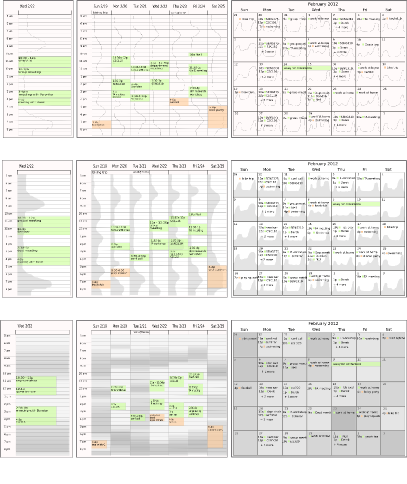
\includegraphics[width=\columnwidth]{figures/proto_incell}
\caption{Design alternatives displayed overlapped (top: line graph; middle: colored region; bottom: luminance)}
\label{fig:incell}
\end{figure}

\begin{figure}
\centering
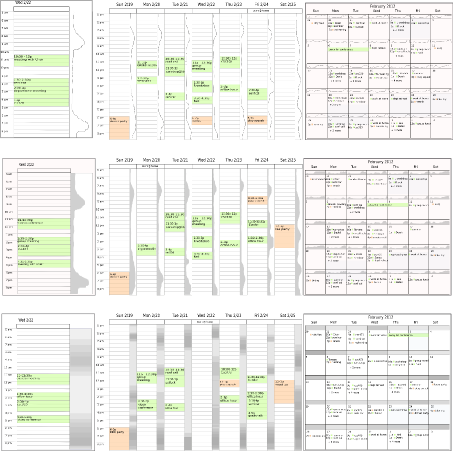
\includegraphics[width=\columnwidth]{figures/proto_inband}
\caption{Design alternatives displayed side by side (top: line graph; middle: colored region; bottom: luminance)}
\label{fig:inband}
\end{figure}

The three visualizations were designed respectively for the typical calendar views: day, week and month (Figure \ref{fig:incell} and Figure \ref{fig:inband}).  Day view is an identical visual encoding to week view.  In month view with luminance, only daily average values were encoded due to the constraint of showing luminance in a small region. In contrast, line chart and colored-region always showed continuous data in all calendar views.

Considering that the overlapped visualization that shares the same space with calendar events and might cause visual interference, another layout alternative is side-by-side display (Figure \ref{fig:inband}) with an additional band parallel with calendar cells, aimed to preserve effective graphical perception while minimizing interference with normal calendar tasks. The width of the visualization band (side-by-side condition) was made smaller than the calendar cell, because the visualizations should not visually dominate the interface.  To enhance the visibility of luminance in overlapped layout, the width of activities (green and orange boxes) is squeezed a little bit compared to other representations to leave a small gap from the boundary (Figure \ref{fig:incell} bottom).  

The early design alternatives were prototyped respective to three criteria: display location (overlapped or side-by-side), visual type (line graph, line graph with shaded color, luminance) and calendar scale (day, week and month views).  However, the viability of supporting attentional ambient in the on-calendar design need to be evaluated and confirmed first (Chapter \ref{chap:viability study}) before they are applied in the field (Chapter \ref{chap:field study}).

%%%%%%%%%%%%%%%%%%%%%%%%%%%%%%%%%%%%%%%%%%%%%%%%%%%%%%%%%%%%%%%%%%%%%%%%%%%%%%%%
%%%%%%%%%%%%%%%%%%%%%%%%%%%%%%%%%%%%%%%%%%%%%%%%%%%%%%%%%%%%%%%%%%%%%%%%%%%%%%%%
%% Chapter - research method
%%%%%%%%%%%%%%%%%%%%%%%%%%%%%%%%%%%%%%%%%%%%%%%%%%%%%%%%%%%%%%%%%%%%%%%%%%%%%%%%
%%%%%%%%%%%%%%%%%%%%%%%%%%%%%%%%%%%%%%%%%%%%%%%%%%%%%%%%%%%%%%%%%%%%%%%%%%%%%%%%

\startchapter{Research Methods}
\label{chap:research methods}
Providing context for reasoning and fitting in with everyday life in order to ease effort were identified as main challenges in personal visualization design (Section \ref{pva:challenges}). With respect to that, this thesis explores the design concept of integrating personal visualization into one's existing information use eco-system.  Specifically, I investigated this concept in the example of integrating visualization of personal feedback data (data about home energy consumption and personal fitness) into one's personal digital calendar, hoping to provide better context to help people interpret their data and lower the barriers involved in accessing these data.  This goal leads to the following research questions that were investigated in the rest of this work.
\begin{enumerate}
	\item{Are the design alternatives comprehensible but not inteferring primary calendar tasks?}
	\item{How do people react and use the on-calendar visualization as the feedback tool in everyday life?}
	\item{To what extent can people use calendar events as context for reasoning about their personal data?}
	\item{Could providing additional context in visualization improve people's understanding of their data?}	
\end{enumerate}

%scope and limitation:
Note that behavior models and their influence on behavior change are out of the scope of this thesis, and the effect of behavior change is not the assessment of the on-calendar approach in this work.  The general philosophy centers around helping people understand their behavior with operational understanding \cite{bartram_design_2015, strengers_designing_2011} rather than digitally lecturing them into behavior change.  We view understanding as a first (but not sufficient) step towards encouraging new habits or taking actions; therefore, tools that can succeed at this step have made progress.

\section{Research Methods}
On the basis of the research questions above, I mainly applied four research approaches in this work: lab experiment, field study, interview and survey. The analysis methods include quantitative statistic analysis and qualitative open coding based on ground theory.  Other than that, two case studies were conducted as pilot studies for the later field study.  The research methods here were considered according to the research phases, contextual factors and related work in previous research.  I will discuss these methods with their benefits and limitation in the following sections, and the further detail are in subsequent chapters.

\subsection{Lab Experiment}
Lab experiment has been commonly used in evaluating information visualization design, in which the often used metrics are completion time, task errors, and even insights \cite{saraiya_evaluation_2004}.
The first phase of this research is to evaluate perceptability and legibility of the design choices (Chapter \ref{chap:viability study}) in facilitating the attentional ambience; that is, visualization on a calendar is perceptible but does not interfere with normal calendar use.  This is the typical perception evaluation in information visualization systems, for example, to evaluate effectiveness of visual channels \cite{mackinlay_automating_1986}, perception of new visualization techniques \cite{heer_sizing_2009}, or visual perception inteferring with background grid \cite{bartram_effect_2011}.
%othe options?

Online experiment may also meet these requirements \cite{cawthon_effect_2007}. However, it may not able to provide contextual information about participants, e.g., through observation. Amazon Mechanical Turk \footnote{https://www.mturk.com/mturk/welcome} is also excluded from being a possible choice due to ethics protocol requirements. 

One concern is that visualization mock-ups (rather than interactive application) were used in the experiment (see Appendix \ref{}), limiting the interaction of participants with the design.  Data encoded in the images were ``hard coded'' (see Section \ref{experiment:design}) and may not reflect real life data patterns.  However, the data pattern and the tasks designed for the tests suit the experiment in perception and interference evaluation, helping to verify the design concept in the early stage.

\subsection{Field Study}
Personal visualization has been often investigated in field study, particularly in HCI community \ref{} and most studies last from one week to one month.  With the working prototype, my interest is to investigate how people react to the on-calendar design in a real life context.  Lab experiment are obviously not suitable in this case (see Section \ref{pva:evaluation}).  Engaging with personal visualization is an ongoing process; it does not require participants' continuous focused attention all the time like usability tasks.  The interaction and reasoning process are embedded in an everyday life context that is impossible to simulate in a lab environment.  With contextual interview only, the ongoing nature would be impossible to investigate.  Randomized Controlled Trial is not proper choice for this research either, since the research questions are open-ended questions about participants experience rather than verifying (or comparing) design solutions (Section \ref{pva:evaluation}). 

This method also has its limitations. The small scale of participants may not enough to represent a statistical effect.  The way people engage with the on-calendar design may vary in different application domains (the analysis focused on personal fitness in this thesis).  Thus, I employ a qualitative method to analyze data from the field study.

\subsection{Survey}
%unintrusive
Survey questionnaire is an unintrusive method to collect data through field study, compared with interviews.  Particularly, self-report surveys for assessment of behavior in natural settings have been widely used \cite{intille_tools_2003}, especially in personal informatics systems \cite{li_stage-based_2010}.  The short questionnaire was used as post-study questionnaire in lab experiments to collect participants' general experience referring to interference, perception and aesthetics.  The weekly survey, a standard instrument to evaluate people's physical activities, was used in field study to evaluate their weekly physical activities.  These data served as supplement for physical activity data collected by wearable devices.  However, a self-reported survey may bring biases (e.g., faulty memories), and participants may forget to fill in the questionnaire in the expected time period.  To address this, I sent reminder emails to participants at the same time every week, and the participants were advised to fill in the questionnaire about the same time every week if possible.

%forget to take, recall bias

\subsection{Interview}
I used interviews to collect data in the field study, gathering information about participants' experience, motivation, and opinions.  This also offers the chance to observe how participants use the visualization application, and investigate their cognitive process of developing insights from data, which might be hard if the data was collected from a survey.  The use of personal visualization is mediated in everyday context is a highly personalized environment, also interacting with culture and social factors (Chapter \ref{chap:pva}). Applying quantitative methods in this case might limit researchers' insight on how and why certain design works. Particularly, in-depth interviews tend to work well with ethnographic methods, e.g., case study or field study \cite{leedy_practical_2012}.  It definitely provides the advantage to investigate open-end questions in research.

%intervention, biased
Inevitably, interviews suffer from bias problems that could be from researchers (e.g., attitude biases) or participants (e.g., recall biases).  Also in a field study, the interview itself may bring intervention effect. Considering that, times of interviews in both research groups (Chapter \ref{chap:field study}) were kept the same to balance the effect.

The interview data were analyzed with quantitative approach based on ground theory through an open coding process \cite{_beliv_2008}. Transcription and observation data were manually tagged.  As patterns and trends of tags were investigated, tags were merged into higher level categories.  As this process was repeated, new models or theories were derived.  This approach is good at analyzing unstructured data, e.g., from interviews, observations, etc., but the caveat is that the coding process may bring in bias from the researcher, e.g., the perspective from which she interprets the data.

\section{Summary}
Generally, evaluating visualizations used in everyday life is difficult and challenging (Section \ref{pva:evaluation}).  The choices of research methods considered in this thesis are based on my research questions.  Specifically, this research is mainly aimed at an investigation of a reflective approach of visualization design in feedback applications. The research methods used in this work are based on this focus.  Potentially, it would be helpful for future research into PV\&PVA.  In the next chapters, I will discuss the two primary studies where these methods applied.



%%%%%%%%%%%%%%%%%%%%%%%%%%%%%%%%%%%%%%%%%%%%%%%%%%%%%%%%%%%%%%%%%%%%%%%%%%%%%%%%
%%%%%%%%%%%%%%%%%%%%%%%%%%%%%%%%%%%%%%%%%%%%%%%%%%%%%%%%%%%%%%%%%%%%%%%%%%%%%%%%
%% Chapter - viability study
%%%%%%%%%%%%%%%%%%%%%%%%%%%%%%%%%%%%%%%%%%%%%%%%%%%%%%%%%%%%%%%%%%%%%%%%%%%%%%%%
%%%%%%%%%%%%%%%%%%%%%%%%%%%%%%%%%%%%%%%%%%%%%%%%%%%%%%%%%%%%%%%%%%%%%%%%%%%%%%%%

\startchapter{Viability Study}
\label{chap:viability study}

As the on-calendar design alternatives are developed based on visualization principles, whether they are valid as expected is still unknown.  To support attentional ambience as embedding a visualization layer into one's calendar, designs need to be visually salient but perceptible.  Controlled lab experiments are a good option to evaluate these perception and legibility criteria (Chapter \ref{chap:research methods}).  In this chapter, I describe the viability study, where I employ lab experiments to evaluate visual interference and perceptability of design alternatives (Chapter \ref{chap:visdesign}).  This stage of my research is to evaluate the idea of on-calendar design approach with proposed alternatives and suggest design options for later implementation.

\section{Background}
The on-calendar approach directly integrates personal time-varying data into a personal digital calendar (i.e. the same calendar that people already use for managing their personal appointments) (Figure \ref{fig:incell},\ref{fig:inband}).  Our design goal is to present information in an unobtrusive way, informing people while blending into the environment and requiring low attentional demand \cite{moere_towards_2007}.  In other words, we ``mash-up'' information sources in a familiar tool (a digital calendar); that is, the additional information is attentionally ambient to avoid interfering with the primary function of the application (i.e., tasks of schedule management). Meanwhile, calendar events can provide context to reason about data patterns that are aligned with them. 

I explore the viability of this approach as the first step to investigate the effectiveness of visualization in this design approach.  Will people accept the idea of having additional data added to their digital calendars?  Can this data be integrated in a way that does not interfere with normal calendar activities, yet enables the data to be perceived? These questions are the focus of this step.  Thus, I investigated visual interference and perceptability of visualization alternatives with lab experiments, and meanwhile aimed to narrow down the design alternatives of on-calendar visualizations for later development. The goal of the experiments here was to identify visual encodings that minimize visual interference with normal calendar tasks, while supporting effective data perception. The experiments in this chapter focuses on these basic design issues related to interference and perceptability rather than other factors influencing sustainable behaviors, such as motivation and social interaction.

\section{Experiment Design}
\label{experiment:design}
Two experiments explored how the following factors that influence visual interference with normal calendar tasks and graphical perception of the quantitative data:(all within-subjects factors in the study):
\begin{itemize}
 \item Display location: overlapped or side-by-side.
 \item Visualization type: line graph, colored-region or luminance. 
 \item Calendar scale: week\footnote{In the viability study, day view was not considered because it would use an identical visual encoding as the week view.}  or month.
\end{itemize}

\subsection{Apparatus}
The experiments were conducted in a controlled usability lab, and images were displayed on a 21'' inch monitor at 1280*1024 resolution.  Static visualization images were created for each combination of the above factors.  I chose static images in the experimental study to minimize the influence of any system delay and to ensure that trials had a clearly defined correct answer.  Trials were presented in random order by a custom Java-based slide-show and data collection program.  Multiple-choice answers were presented in a new page after the participant had done the visual search or data interpretation, so time to input the answer was not included in the timing measures.
The schedule in the experiments was a sample schedule from a faculty member, and the energy data (electricity usage) were ``hard coded'' according to each of the tasks. To prevent color effects, all visualizations were in grey (or with luminance varied). The colored calendar event blocks on the calendar were semi-transparent (with alpha level at 0.6).

\subsection{Participants}
Thirty one participants were recruited (14 female, 17 male) including undergrad and graduate students, with a diversity of backgrounds (computer science, engineering, chemistry, biology, education, social science and political science). Fifteen of them participated in the first experiment and 16 participated in the second one.

\subsection {Experiment I: Calendar Tasks}
Experiment I investigated the interference of visualizations with normal calendar tasks.  Tasks were designed to involve only visual search, to eliminate any individual differences in interaction speed, such as event editing or text input.  We also chose to investigate visual search tasks because they are the most likely to suffer from interference from the addition of background data displays.  Participants were asked to search for a single event (e.g., ``What time is the group meeting?'') or count repeated events (e.g., ``How many seminars do you have in the week/month?''), without being informed about the additional data layer in advance (see the full list of task questions in Appendix \ref{}). 

Experiment I was to test the following hypotheses:
\begin{itemize}
\item{Visualizations displayed in overlapped position would have greater interference than visualizations displayed side by side(H1.1).} 
\item{Line graph would interfere with calendar activities the least and luminance would interfere the most (H1.2), since luminance would take the most space on the calendar background and line graph would take the least.}
\end{itemize}

\section {Experiment II: Visualization Tasks}
The second experiment investigated the graphical perception of visualizations on a calendar; that is, how people interpret the meaning of data patterns.  Participants were asked to complete tasks that involved perceiving general patterns from the visualizations, but not precise values.  The tasks were derived from established temporal data tasks described in the literature.  Saraiya et al. suggested that people would get insights from overview, patterns, groups and details \cite{saraiya_evaluation_2004}.  Furthermore, elementary (local patterns or extreme values) and synoptic tasks (overall estimate or distribution) are typical ways to explore temporal data \cite{andrienko_exploratory_2006}.  Thus we included tasks that involved investigating local patterns and estimating overall summaries.  For instance, participants were asked to interpret the energy consumption spikes (e.g., ``What day do things start the latest in the morning?''), local patterns (e.g., ``Which evening do you consume the most energy from 7pm to 9pm?'') and compare summaries of days (e.g., ``Do you consume more energy on Tuesday than Thursday?''). The full list of task questions is included in Appendix \ref{}.

Experiment II was to test the following hypotheses:
\begin{itemize}
\item{Visualizations displayed side by side would be easier to perceive than  visualizations in overlapped position (H2.1), since side-by-side visualizations do not have calendar activities occluding the data representation} 
\item{Colored-region would be easier to perceive than luminance or line graph (H2.2), considering position encoding is a stronger visual cue than luminance encoding and color difference would enhance visibility of the contour.}
\end{itemize}

\section {Procedure}
Each of the participants completed a set of trials comprised of all combinations of the three factors (visualization type, display location, and calendar scale) for one of the two experiments.  All trials were presented in a random order.  Three practice trials were presented prior to the main trials.  In Experiment I, an additional set of trials was included for a control condition that had no visualization on the background; control trials were also in random order, intermixed with the other trials.

\section{Experiment Results}
In the viability lab study, task time and task accuracy were set as the measures. Task time was defined as the time period only for viewing the images, and did not include the time of answer input (via multiple choice). Accuracy rate refers to the percentage of tasks completed correctly.

Data of the two experiments were analyzed with respect to three factors: display location (overlapped or side-by-side), visualization type (colored-region, luminance or line graph), and calendar scale (month or week view). Task time was tested with repeated measures ANOVA followed by pairwise comparisons, as the data were confirmed to fit a normal distribution via Q-Q plots. All post hoc comparisons used Bonferroni correction. Accuracy was analyzed with Cochran’s Q due to its binomial distribution, followed by Bonferroni-corrected McNemar's tests for pairwise comparisons. For the control condition in Experiment I, I used Bonferroni corrected paired comparisons to compare the control condition task time to each combination of Visualization Type and Display Location.

\subsection{Experiment I: Visual Interference}
\subsubsection{Visualization Conditions vs. Control Condition}

Accuracy rates are shown in Table \ref{table:accuracy}. There was an overall significant difference in accuracy across conditions (\textit{Q}(6) = 34.08, \textit{p} \textless 0.01) in Experiment I. When comparing visualization conditions to the control, McNemar's tests showed that task accuracy was significantly lower with overlapped colored-region than the control condition (\textit{p} \textless 0.04), and with overlapped line graph compared to the control (\textit{p} \textless 0.01). The other conditions were not significantly different than the control. None of the visualization conditions was significantly different than the control condition for task time (shown in Figure ~\ref{fig:lab_control}).

\begin{table} 
\begin{center}
\begin{tabular}{rrcc}
\hline
 Display   &  Encoding  &  Experiment I   &   Experiment II   \\
\hline
 side-by-side   &    line graph      &  90     &  78  \\
                &    colored-region  &  80     &  87  \\
                &    luminance       &  87     &  84  \\
\hline
 overlapped     &    line graph      &  40\textsuperscript{*}      &  44  \\
                &    colored-region  &  53\textsuperscript{*}     &  87  \\
                &    luminance       &  87     &  97  \\
\hline
\multicolumn{4}{l}{\textsuperscript{*}\footnotesize{Significant difference compared with the control condition}}
\end{tabular}
\caption{Accuracy Rates (\%)}
\label{table:accuracy}

\end{center}
\end{table}



\subsubsection{Visualization conditions}

\textbf{Task time}: The three-factor ANOVA analysis showed a significant main effect for Visualization Type (\textit{F}(2,28) = 6.00, \textit{p} \textless 0.02, $\eta^2$=0.30) and a significant main effect for Calendar Scale (\textit{F}(1,14)= 194.89, \textit{p} \textless 0.01, $\eta^2$=0.93) but no significant main effect for Display Location (\textit{F}(1,14)=4.07, \textit{p} \textless 0.07, $\eta^2$=0.23). There were no significant interactions. 

Overlapped visualizations (M=17.17, SD=7.84) took slightly more task time than side-by-side visualizations (M=16.16, SD=7.41), as shown in Figure ~\ref{fig:lab_control}. Pairwise comparisons between groups of Visualization Type showed that line graph took significantly more task time than colored-region (\textit{p} \textless 0.02). Participants spent significantly more task time with month view than week view (not shown).

\textbf{Accuracy}:
The side-by-side conditions had higher accuracy rate (86\%) than overlapped (60\%), (\textit{Q}(1) = 15.11, \textit{p} \textless 0.01, see Table \ref{table:accuracy}). With both side-by-side and overlapped conditions, the accuracy rate was 87\% with luminance, 65\% with line graph and 65\% with colored-region, (\textit{Q}(6) = 34.08, \textit{p} \textless 0.01). Pairwise comparisons with McNemar's tests showed that luminance had significantly higher accuracy than line graph (\textit{p}  \textless 0.03). Accuracy rate was significantly lower in month view (64\%) than in week view (81\%)(\textit{Q}(1) = 6.82, \textit{p}  \textless 0.02).


\begin{figure}[h]
\centering
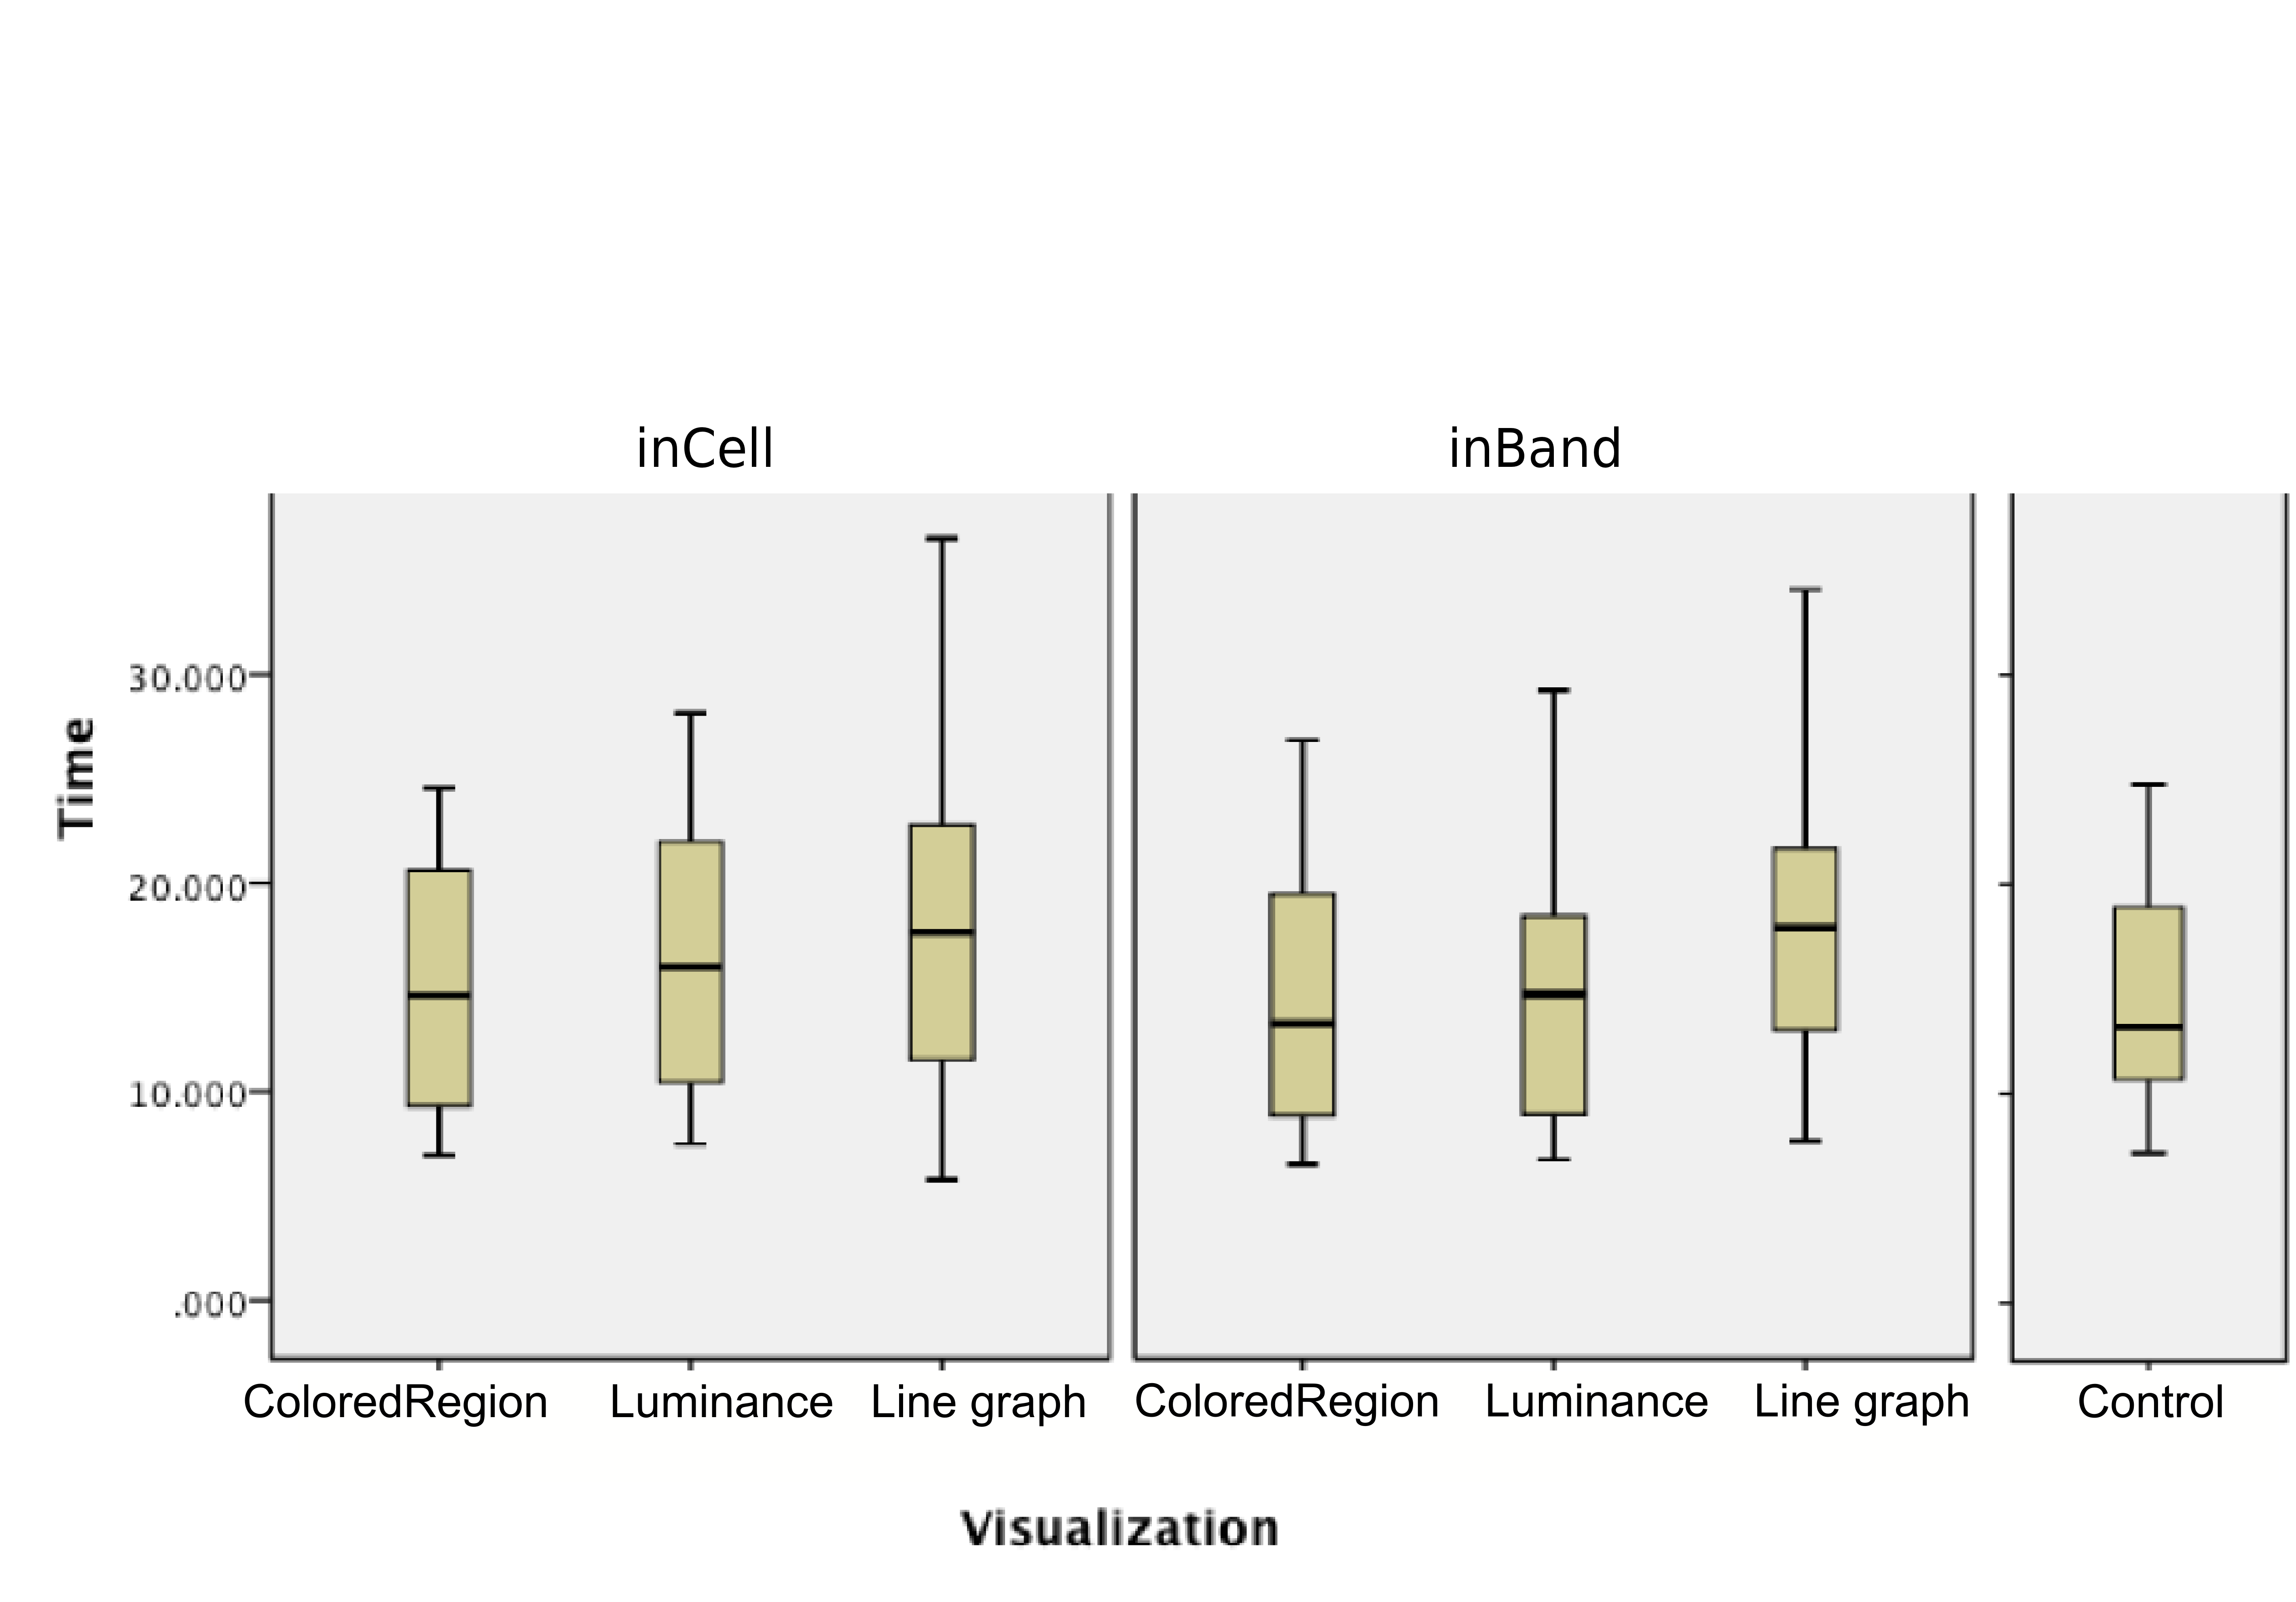
\includegraphics[width=\columnwidth]{figures/lab_control}
\caption{Boxplots showing task time of Experiment I)}
\label{fig:lab_control}
\end{figure}

\subsubsection{Summary of Experiment I}

Colored-region and line graph visualizations caused minor interference with task accuracy when located overlapped, but luminance and side-by-side visualizations had no observable interference. Among the visualization types, line graph caused greater interference than the others as measured by both time and accuracy.

\subsection{Experiment II: Graphical Perception}

\textbf{Task time}:
Response times for Experiment II are summarized in Figure \ref{fig:lab_exp2}. The three-factor ANOVA analysis revealed a significant main effect for Display Location (\textit{F}(1,15) = 10.51, \textit{p} \textless 0.01, $\eta^2$ = 0.41), and a significant main effect for Visualization Type (\textit{F}(2,30) = 10.72, \textit{p} \textless 0.01, $\eta^2$ = 0.42), but no significant main effect for Calendar Scale,(\textit{F}(1,15) = 2.72, \textit{p} \textless 0.12, $\eta^2$ = .15). The interaction between Visualization Type and Time Scale was significant (\textit{F}(2,30) = 6.72, \textit{p} \textless 0.01, $\eta^2$ = .31). Other interactions were not significant.

The overlapped condition (M=10.03, SD=8.29) took significantly less task time than the side-by-side condition (M=13.02, SD=8.81), as shown in Figure 3. Pairwise comparisons showed that luminance took significantly less task time than colored-region (\textit{p} \textless 0.01) and line graph (\textit{p} \textless 0. 01), but this difference occurred only in month view, not in week view. Recall that luminance in month view represented aggregated information (daily average), a possible explanation for this difference.

\begin{figure}[h]
\centering
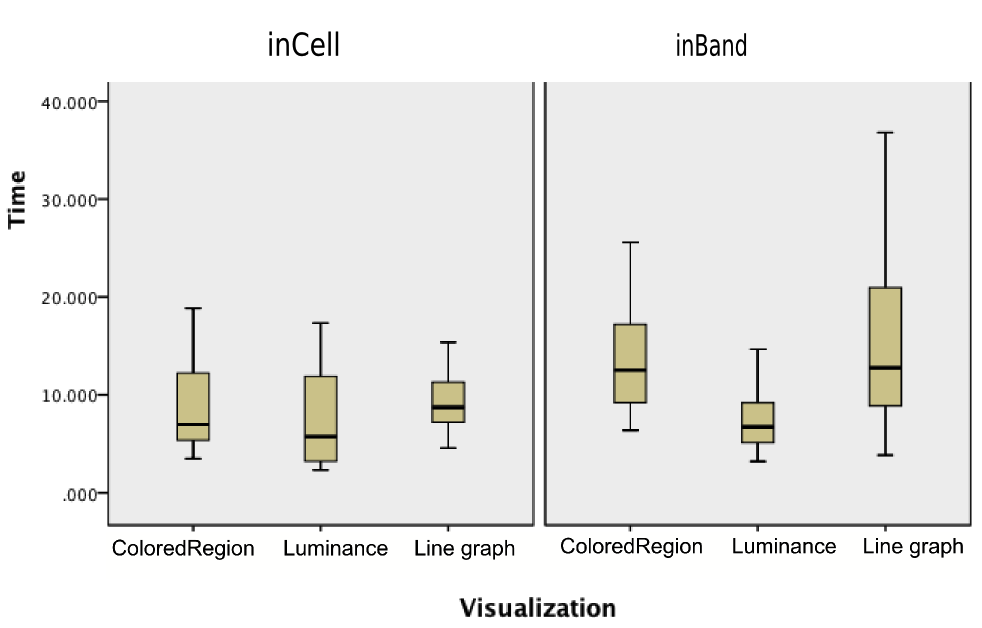
\includegraphics[width=\columnwidth]{figures/lab_exp2}
\caption{Boxplots showing task time of Experiment II)}
\label{fig:lab_exp2}
\end{figure}

\textbf{Accuracy}:
the accuracy rate was 76\% with the overlapped condition and 83\% with the side-by-side condition, but these were not significantly different (\textit{Q}(1) = 1.82, \textit{p} \textless  0.18, see Table \ref{table:accuracy}). With both side-by-side and overlapped conditions the accuracy rate was 87\% with colored-region, 90\% with luminance and 61\% with line graph, with a significant effect (\textit{Q}(2) = 20.44, \textit{p} \textless  0. 01). Pairwise comparisons with McNemar's tests showed that line graph had significantly lower accuracy than luminance (\textit{p} \textless  0.01) and colored-region (\textit{p} \textless  0.01). Accuracy was particularly low with line graph when it was located overlapped (44\%). With respect to temporal scales, the accuracy rate was 85\% in month view and 74\% in week view, not a significant difference (\textit{Q}(1) = 4.17, \textit{p} \textless  0.41).


\subsubsection{Summary of Experiment II}
The overlapped condition facilitated better graphical perception than the side-by-side condition. Luminance was easier to perceive than colored- region and line graph (as measured by task time), possibly because of the data aggregation in month view. Line graph was the most difficult to perceive (it had lower task accuracy).


\subsection{Post-study Questionnaire}
Participants were asked to fill in a questionnaire after the experiments, with respect to their experience of visual distraction, graphical perception and aesthetics. Those questions were likert scale ratings that were analyzed with repeated measures ANOVA after it was confirmed to match to a normal distribution via Q-Q plots. Post hoc comparisons used Bonferroni correction.

\begin{figure}
\centering
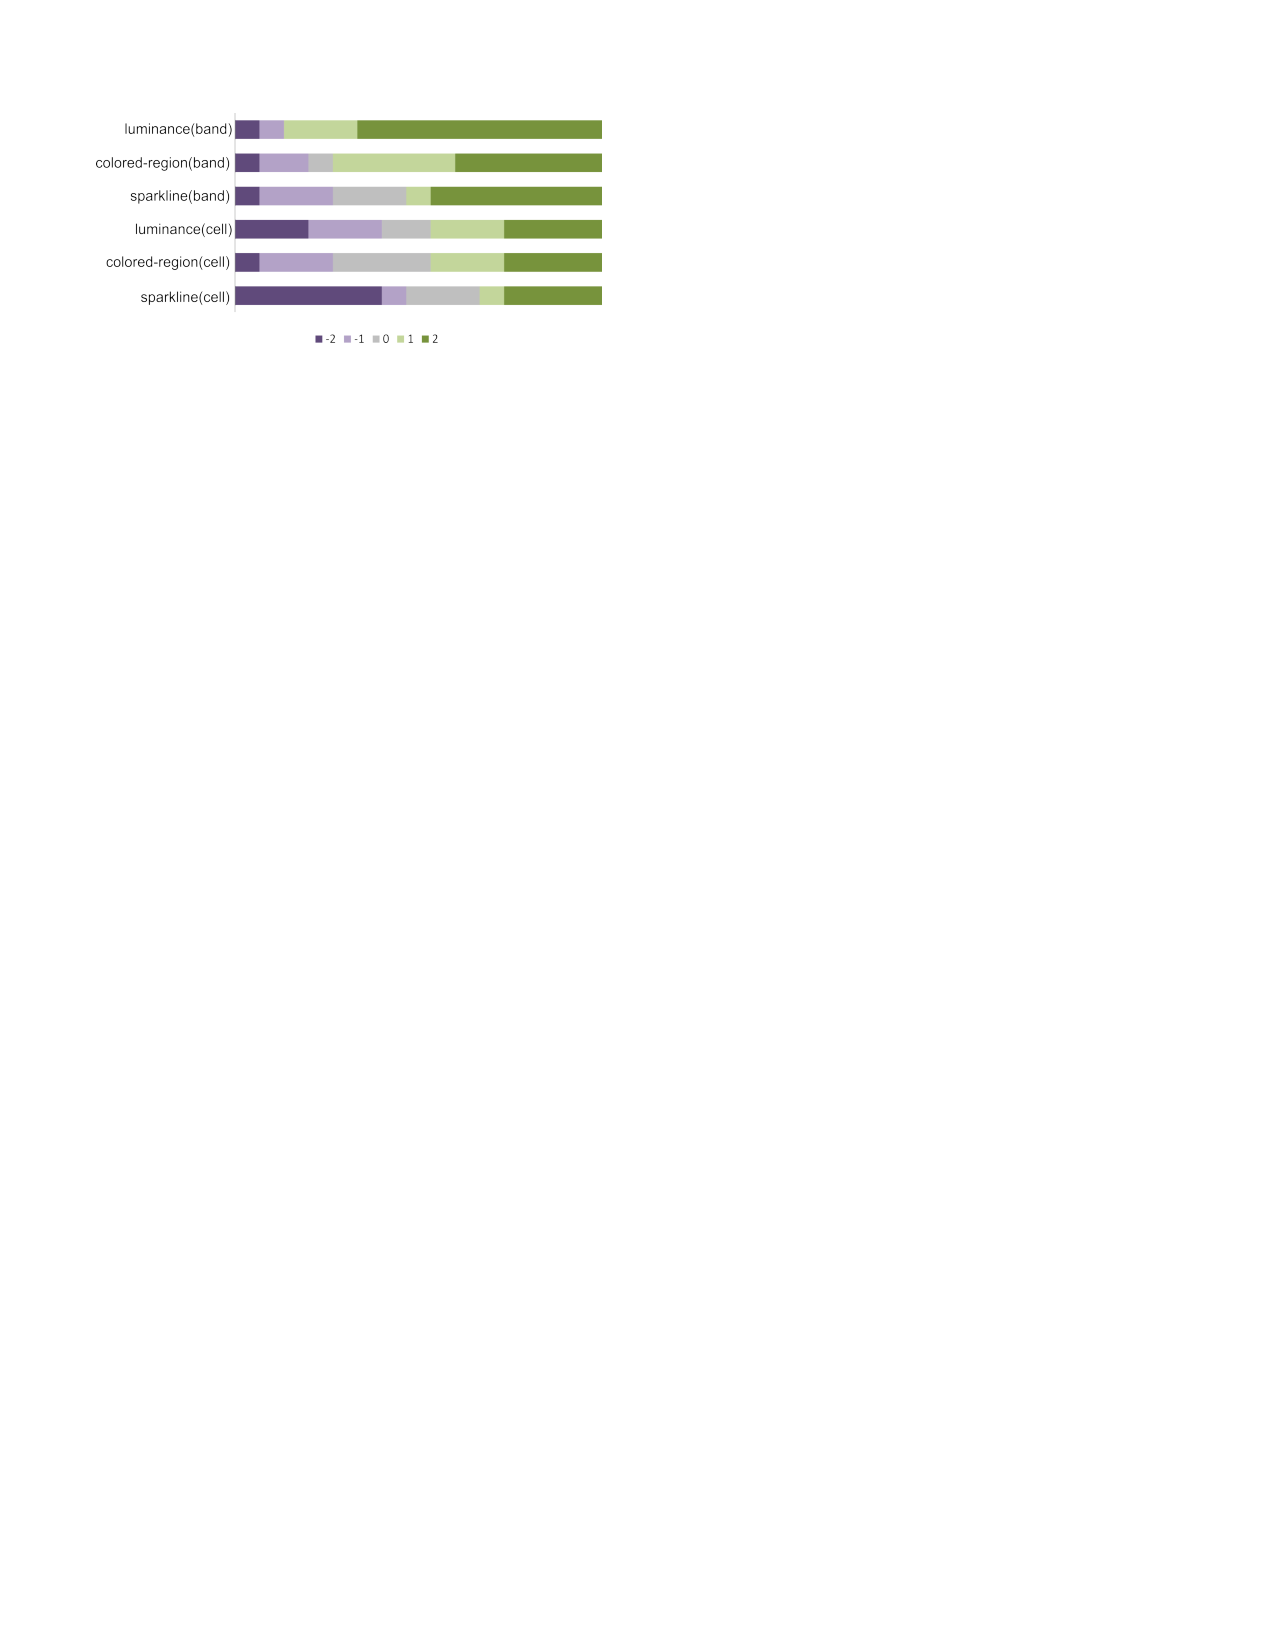
\includegraphics[width=\columnwidth]{figures/rating_distraction}
\caption{ Visual distraction reported by participants (-2 is ``very distracting'', 2 is ``not distracting'')}
\label{fig:rating_distraction}
\end{figure}

\begin{figure}
\centering
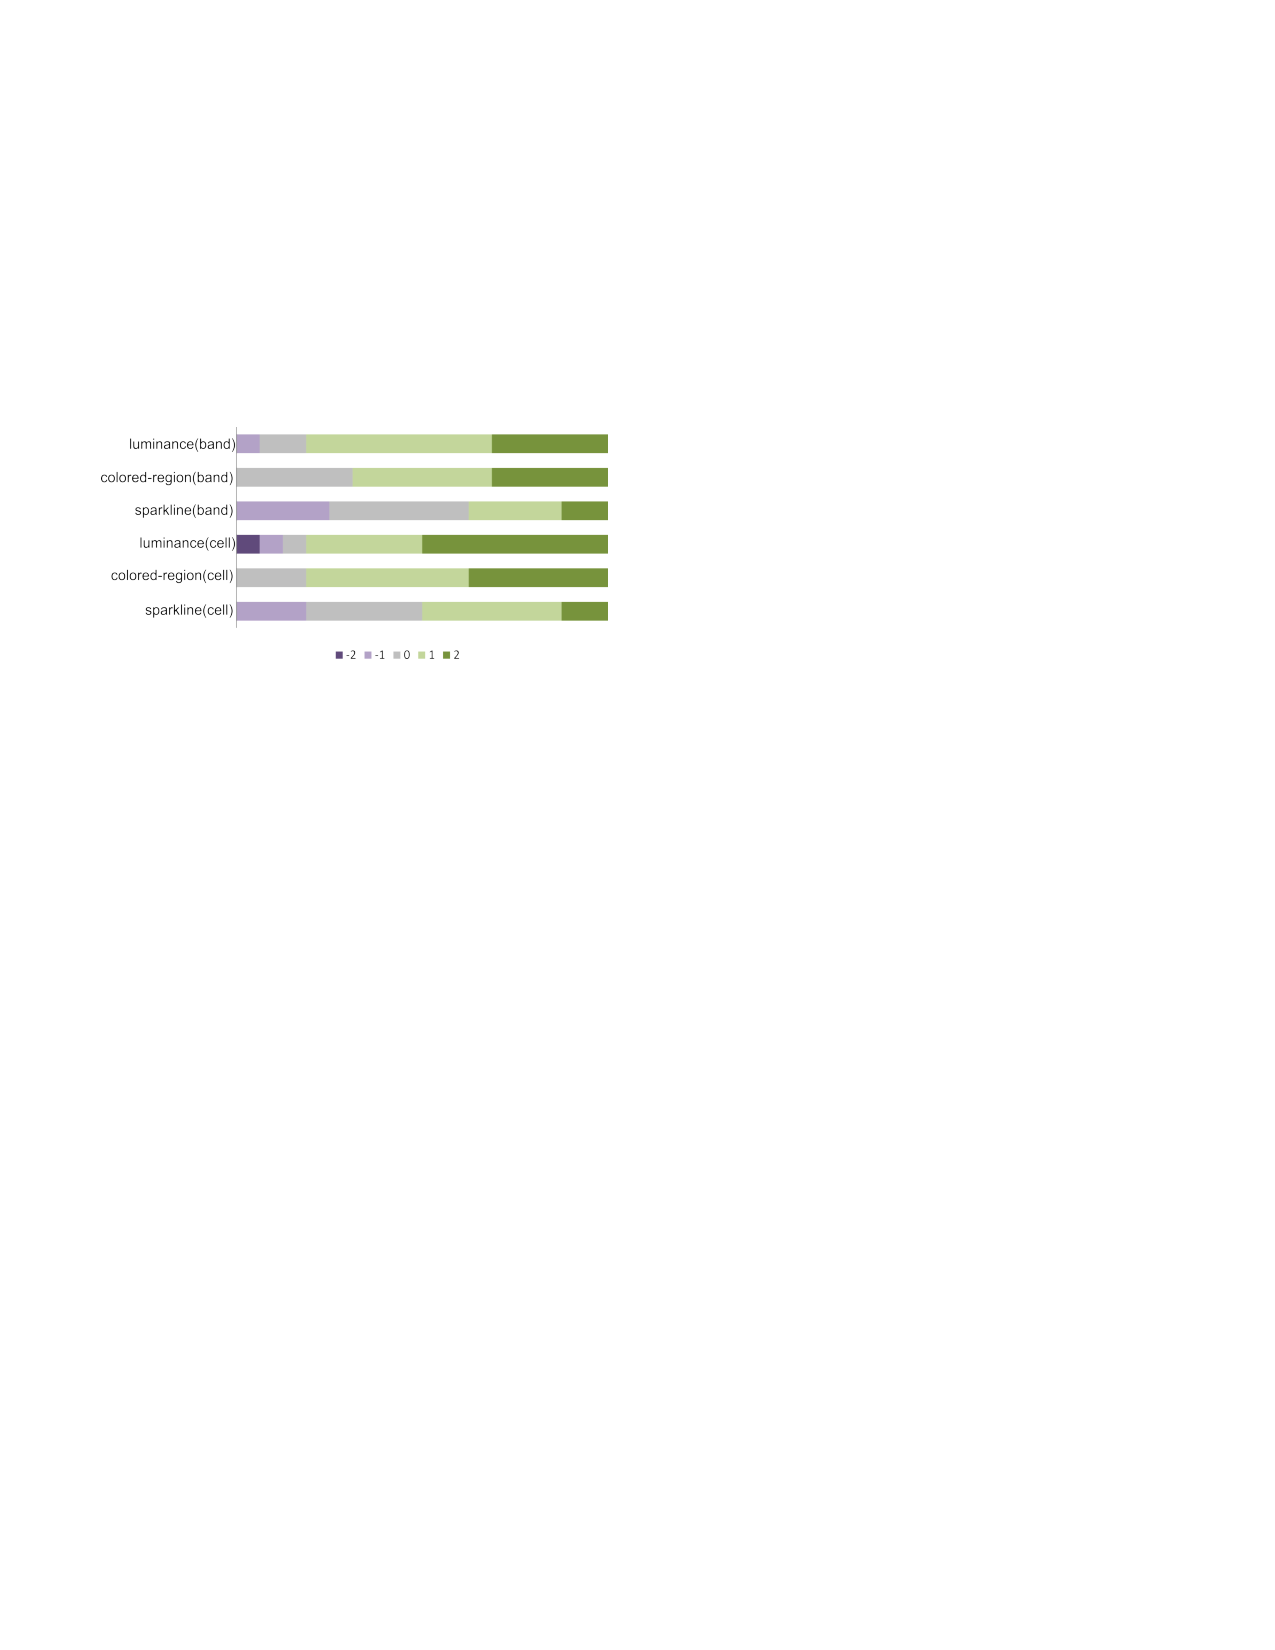
\includegraphics[width=\columnwidth]{figures/rating_perception}
\caption{ Graphical perception reported by participants (-2 is ``very difficult'' and 2 is ``very easy'').}
\label{fig:rating_perception}
\end{figure}

\begin{figure}
\centering
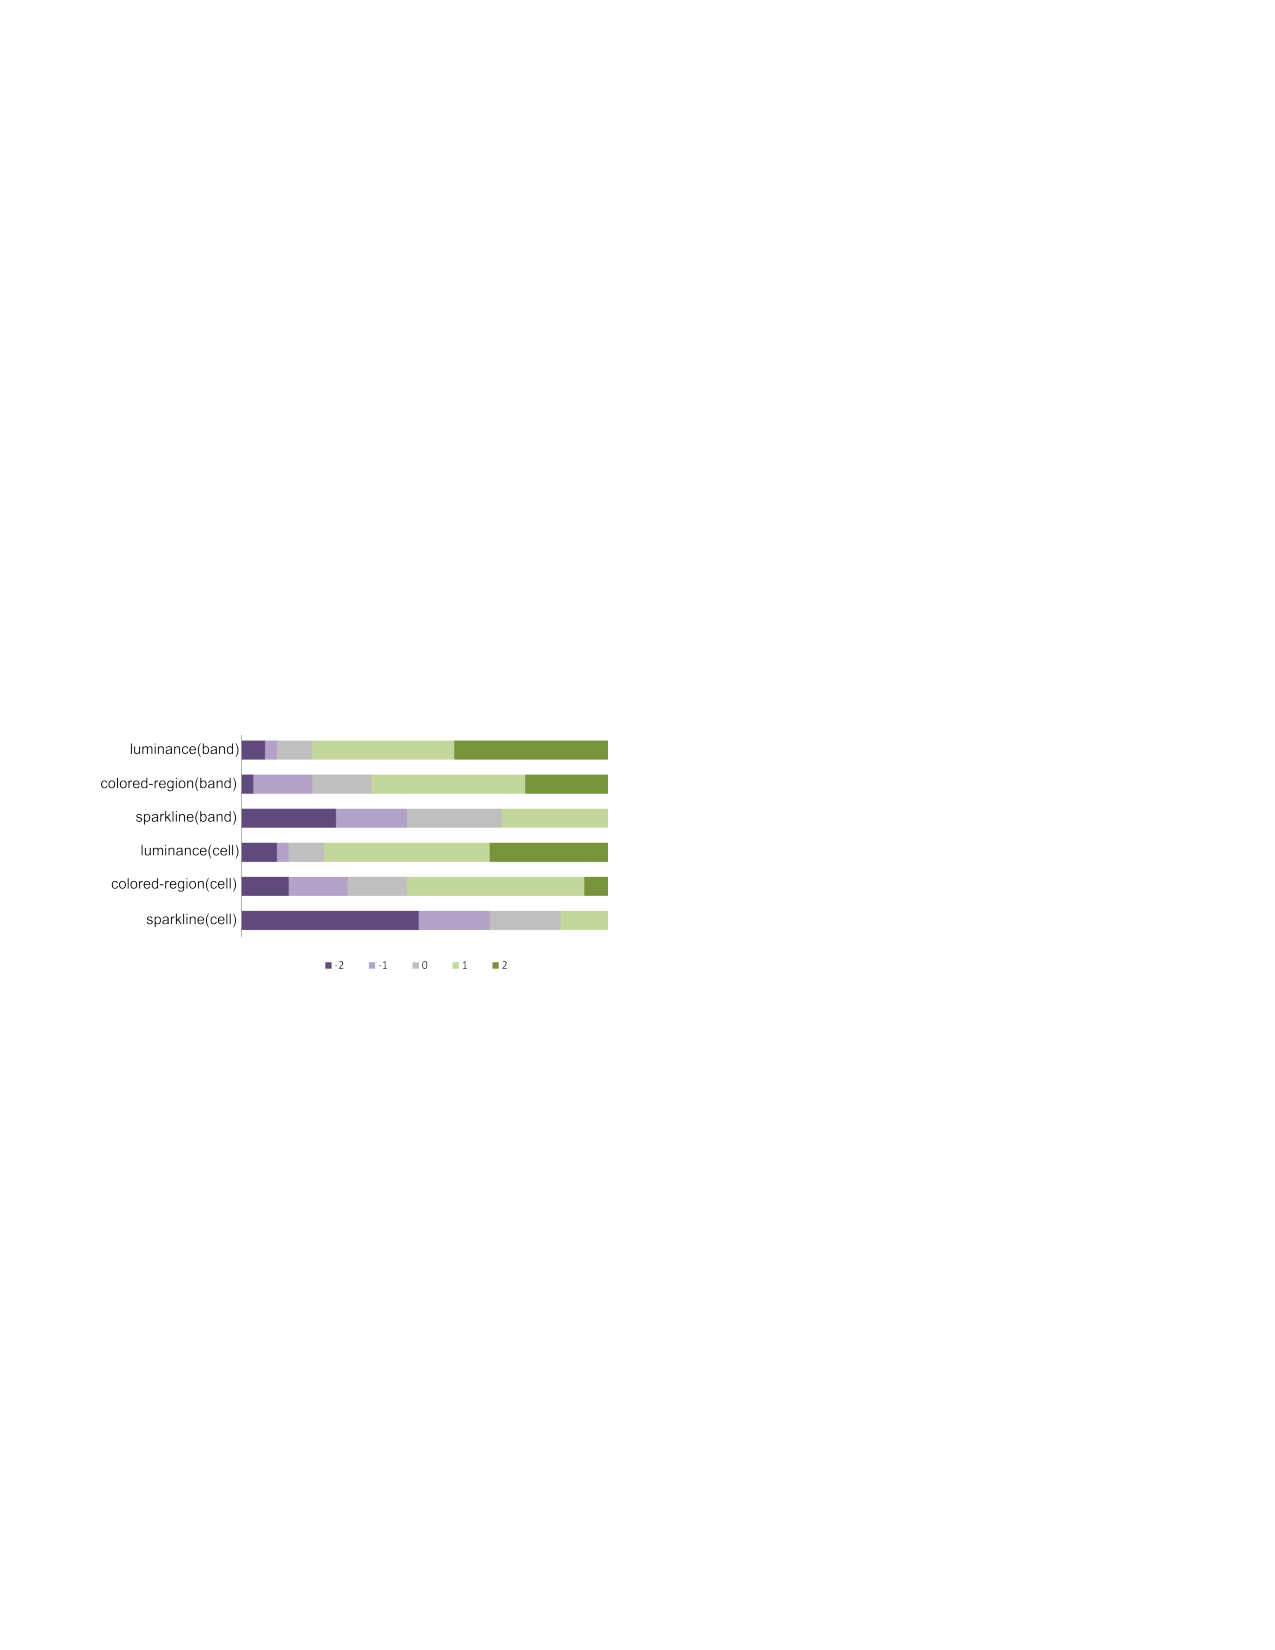
\includegraphics[width=\columnwidth]{figures/rating_aesthetics}
\caption{ Aesthetics reported by participants (-2 represents ``very poor'' and 2 represents ``very good'')}
\label{fig:rating_aesthetics}
\end{figure}

\subsubsection{Visual Distraction}
As shown in Figure \ref{fig:rating_distraction}, participants in Experiment I rated the in-cell condition more distracting than the in-band condition, and line graph was rated more distracting than colored-region and luminance. We found a significant main effect of Display Location (\textit{F}(1,14)=8.90, \textit{p} = 0.01, $\eta^2$= 0.39), but not Visualization Type. The interaction was not significant. Participants also reported that they could not stop being visually distracted by sparkline, particularly with the in-cell condition.

\subsubsection{Graphical Perception}
As shown in Figure \ref{fig:rating_perception}, participants in Experiment II rated the in-cell condition as easier to perceive than the in-band condition. Line graph was rated the most difficult visualization to perceive. We found a significant main effect of Visualization Type (\textit{F}(2,30)=.04,  \textit{p} =3.72,  $\eta^2$ =.20), but not Display Location. The interaction was not significant. Pairwise comparisons showed that colored-region was rated significantly better than sparkline (\textit{p} \textless 0.01).

\subsubsection{Aesthetics}
In-band visualizations were rated more appealing than in-cell visualizations, and sparkline was rated the least appealing visualization (Figure \ref{fig:rating_aesthetics}). There were significant main effects of Display Location (\textit{F}(1,30)=5.15, \textit{p} =0 .03, $\eta^2$ = 0.15) and Visualization Type (\textit{F}(2,60)=26.19, \textit{p} \textless 0.01, $\eta^2$ = 0.47). The interaction was not significant. Pairwise comparisons showed that sparkline was rated significantly lower than colored-region (\textit{p} \textless 0.01) and luminance (\textit{p} \textless 0.01).

\subsubsection{Summary}
User ratings confirmed the performance findings: in-cell visualizations had greater interference with calendar operations than in-band ones, but data was easier to perceive with in-cell visualizations. Sparkline was rated the most interfering and the most difficult visualization to perceive. Considering aesthetics, in-band visualizations were preferred over in-cell visualizations, and colored- region and luminance were preferred over sparkline.


\section{Discussion of Lab Experiment Results}
\subsection{Interference (Experiment I)}
The hypothesis (H1.1) that in-cell visualizations would have greater interference with calendar activities compared to in-band was confirmed. In Experiment I, task time was slightly faster with in-band visualizations and accuracy was significantly higher. However, presence of quantitative visualizations on a calendar did not greatly compromise the regular calendar tasks. Although the results showed a drawback of in-cell visualizations for calendar task accuracy (mostly from line graph), there were no significant differences in task time between the control condition and the visualization conditions. 

The hypothesis (H2.1) that in-band visualizations would be easier to perceive than in-cell ones was not confirmed. On the contrary, in-cell visualizations were easier to perceive than in-band ones. The presence of calendar activities in the same space did not compromise performance at graphical perception.

\subsection{Perception (Experiment II)}

As hypothesized, line graph would interfere with calendar activities the least and luminance would interfere the most (H1.2). This hypothesis was not confirmed; in fact it was directly contradicted. Task time with line graph was significantly longer and its error rate was significantly higher than the others. Participants also qualitatively reported that line graph caused greater interference than colored-region and luminance. I speculate that this interference might be caused by the similar color (grey) of the line graph and activity text, which could make reading the text more difficult. With colored-region, the filled color area tones down the interference to some degree. Thus, we eliminated line graph as a visualization option in our later implementation.

The hypothesis (H2.2) that colored-region would be easier to perceive than the others was not confirmed either. Luminance had higher accuracy than line graph and was faster than both other visualizations in month view. The advantage of color coding was observed in small graph scales (month view) but not in large graph scales (week view). I strongly suspect that this is due to aggregation: luminance in month view encoded daily average value while line graph and colored-region represented continuous daily data.

\subsection{Design Implications}
These results indicate the viability of compositing quantitative data into a typical calendar view without compromising the effectiveness of either the data visualization or the calendar itself, but they also highlight a number of design implications and issues. Foremost, it seems clear that there is not a ``one size fits all'' solution. Even in the small set of factors we considered in the study, certain visualizations fit better at different calendar scales and in different calendar codings. For example, the performance of luminance, in which we filled the entire cell with a gray scale representing a single aggregate value, was most effective in the month view; its superiority to the colored-region in the week view was insignificant. The continuous encoding in week view provides a finer resolution of the data (and is reported qualitatively as moderately less distracting). However, luminance in the week view may interfere with the color coding the user has applied to her personalized calendar entries, whereas these entries in the month view are typically presented as text, so filling the cell could be less interfering. In addition, there are a limited number of discriminable levels in gray scales, thus reducing the resolution of the visualization. Thus the usability principle of consistent coding may be ineffective here: adaptive visualization, where the representation takes a different form according to the scale of the calendar and the desired granularity of the data, better fits the goals of clarity and visual non-interference. Based on this, we offer some design suggestions to optimize visualization of quantitative data on a calendar.

In-cell visualizations support better graphical perception with the sacrifice of minor interference, compared to in-band visualizations. Therefore, in-cell approaches might be the better default design choice, especially for small devices where screen space is very limited. However, in-cell visualizations may not extend well to situations where the calendar is extremely dense (e.g. back to back meetings all day); in this case, in-band could be a viable alternative.

\subsection{Attentional Ambience}
This work introduced the concept of attentional ambience as an extension to ambient visualizations. Attentional ambience is defined by the degree to which the representation can exist in a visual middle ground where features can be pulled into the foreground or relegated to the background by slightly changing the degree of attention \cite{bartram_effect_2011}. It is this capacity of our visual system that supports the kinds of information mash-ups proposed in this paper.

Limitations in the study scope encourage further investigation. I did not, for example, consider device size nor context of use (mobile vs. fixed). Clearly these different conditions will influence the degree of visual saliency or subtlety that is most effective for attentional ambience. The focus of this study was to investigate the degree of visual salience that provides the best balance between ambience and perceptual efficiency for the two conditions (colored region and luminance), as they seem the most promising. The alpha level used in both was 0.6, but previous research in overlaid structures suggests that we can use a much more subtle level of 0.2 to provide a ``just attendable difference'' \cite{bartram_effect_2011} between the two data sets. Possibly, a lower opacity of the quantitative data might have positively affected the calendar accuracy results without compromising the quantitative interpretation. Thus, the opacity of visualization could be customized to better support attentional ambience. Particularly in this case, attentional ambience would be influenced by the characteristics of individuals' calendar as well, e.g., the density of calendar events displayed, existing color used to code events, etc.

Moreover, the ``appropriate'' levels of attentional ambience introduces new design options.  There may be thresholds at which the visual salience should be increased: for example, high blood glucose levels (diabetes data) or energy consumption spikes that exceed a daily average. We believe this approach may thus support both informed historical analysis and near-real-time monitoring and alerting tasks.



%%%%%%%%%%%%%%%%%%%%%%%%%%%%%%%%%%%%%%%%%%%%%%%%%%%%%%%%%%%%%%%%%%%%%%%%%%%%%%%%
%%%%%%%%%%%%%%%%%%%%%%%%%%%%%%%%%%%%%%%%%%%%%%%%%%%%%%%%%%%%%%%%%%%%%%%%%%%%%%%%
%% Chapter - Implementation
%%%%%%%%%%%%%%%%%%%%%%%%%%%%%%%%%%%%%%%%%%%%%%%%%%%%%%%%%%%%%%%%%%%%%%%%%%%%%%%%
%%%%%%%%%%%%%%%%%%%%%%%%%%%%%%%%%%%%%%%%%%%%%%%%%%%%%%%%%%%%%%%%%%%%%%%%%%%%%%%%

\startchapter{Implementation}
\label{chap:implementaiton}

Following the lab study, I implemented a working prototype as an interactive web application (Figure \ref{fig:implementation1}). The lab study results suggest to remove line graph from the visualization alternatives because it caused significant interference between the visualization layer (additional data stream) and calendar events. The implementation kept the other visual encodings because they all seemed viable and I wanted to see which ones people would prefer in practice. 


\begin{figure}[h]
\centering
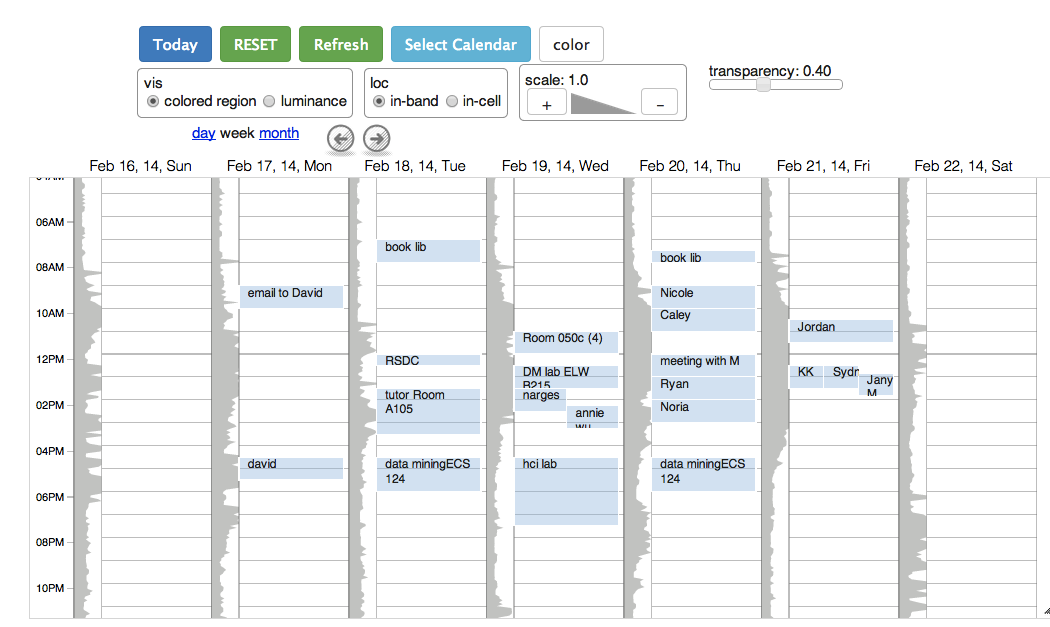
\includegraphics[width=\columnwidth]{figures/implementation1}
\caption{web application of on-calendar visualization using Google calendar API and displaying household smart meter data.}
\label{fig:implementation1}
\end{figure}

The web application basically works as an online digital calendar, synchronizing with calendar events (through Google API \footnote{https://developers.google.com/google-apps/calendar/}) and also fetching live data feeds (from a household smart meter or Fitbit data API \footnote{https://dev.fitbit.com/}) \ref{fig:system}. The web application was implemented with PHP and Javascript, and the visualization layer was implemented with D3.js \footnote{https://d3js.org/}. It could be run on desktop (or laptop), tablet and mobile phone with a browser, but the layout was designed for desktop browser size (it was not customized for mobile devices). The application was hosted on the server at Simon Fraser University.

\begin{figure}[h]
\centering
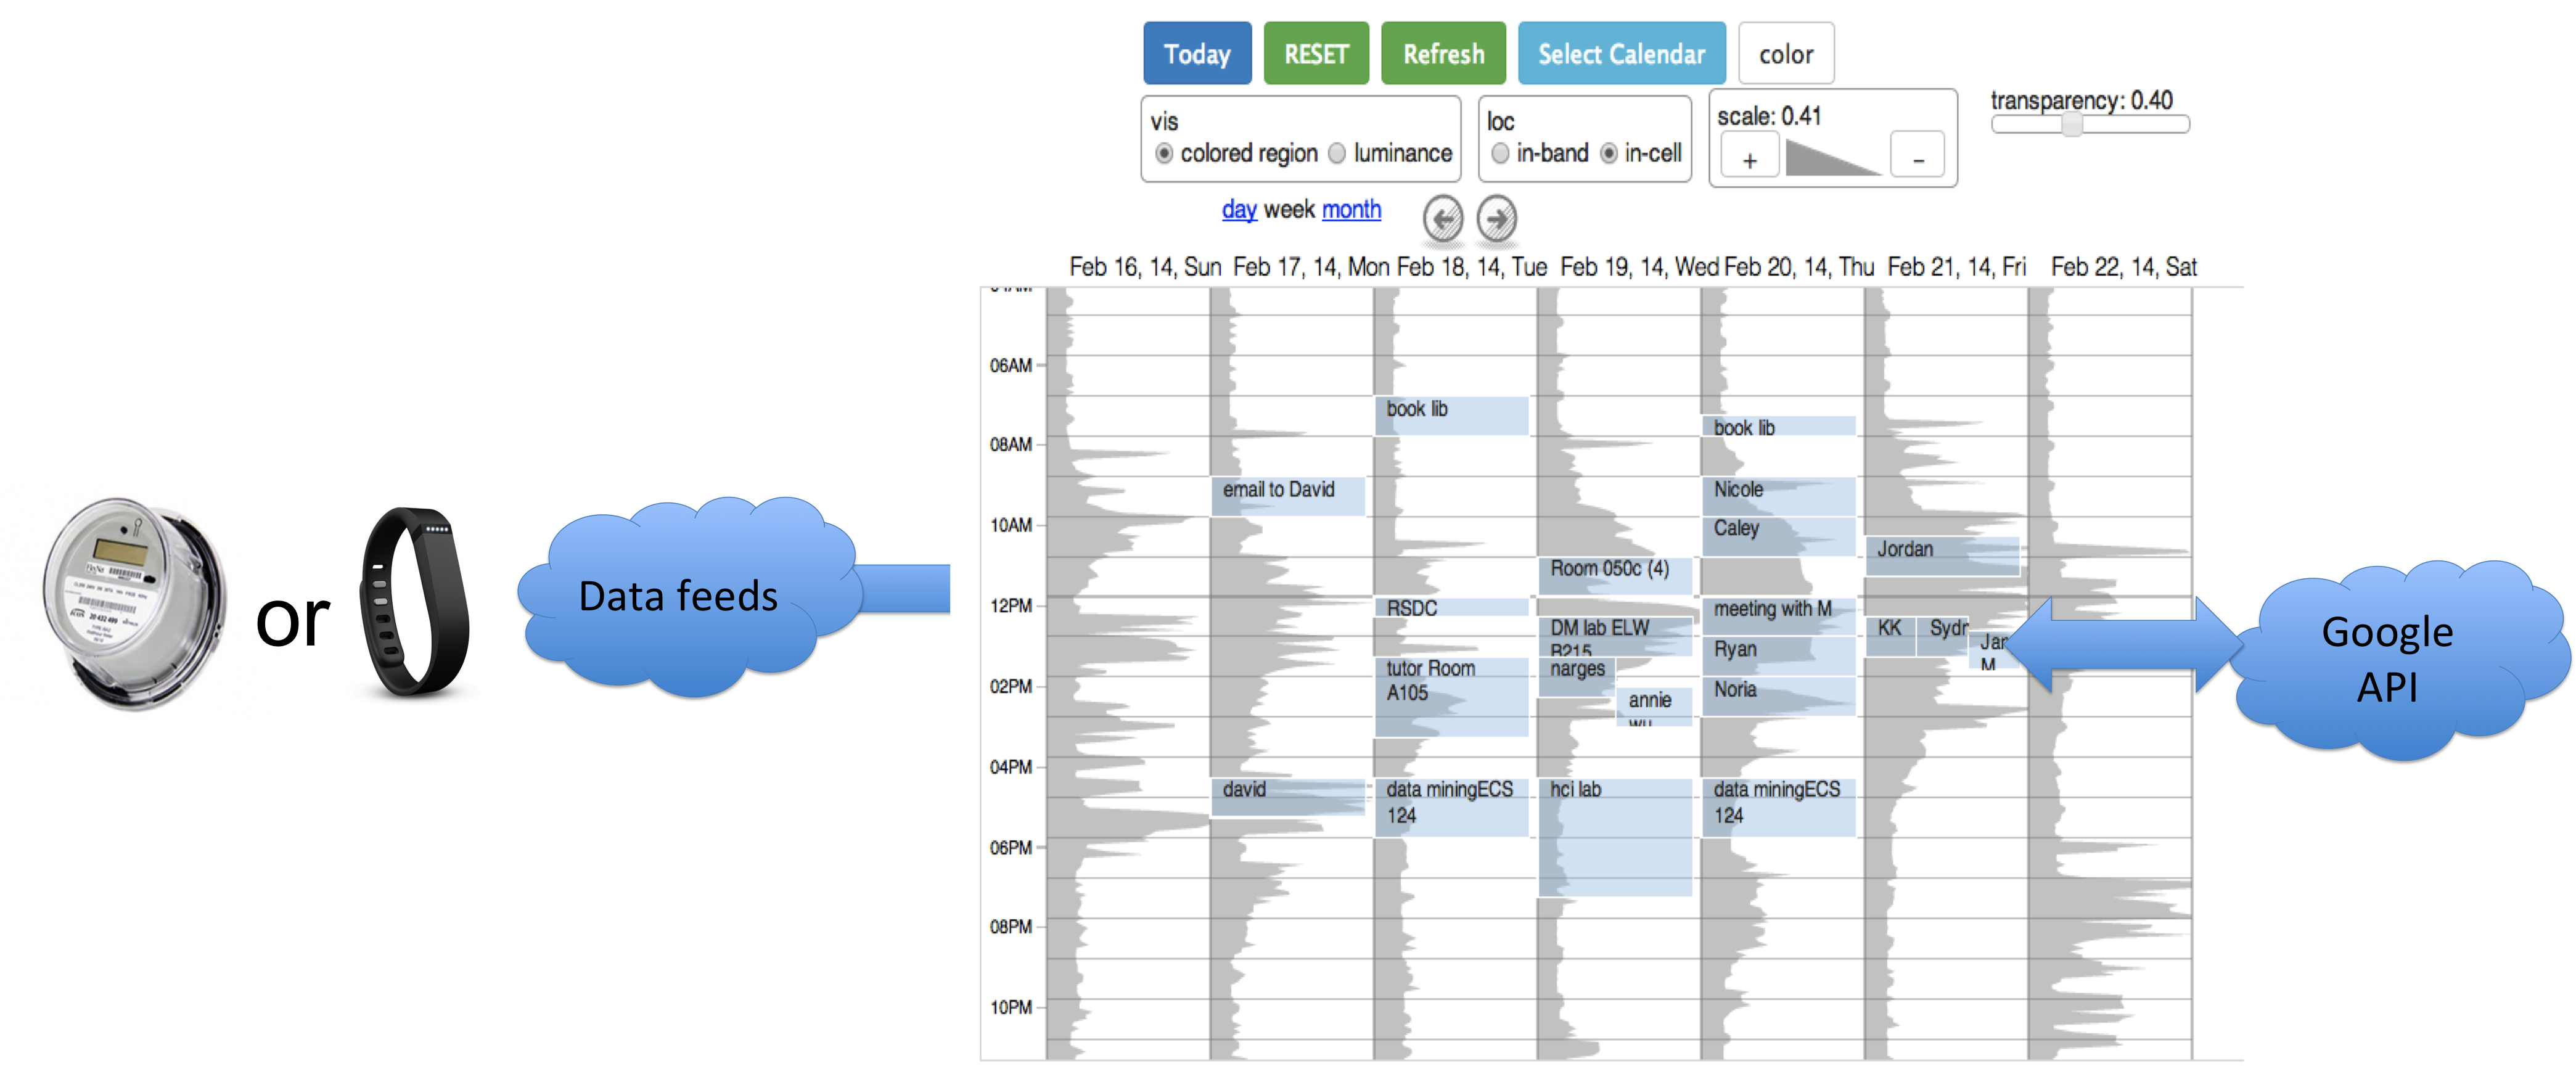
\includegraphics[width=\columnwidth]{figures/system}
\caption{Data flow of the on-calendar visualization system.}
\label{fig:system}
\end{figure}


\begin{figure}[h]
\centering
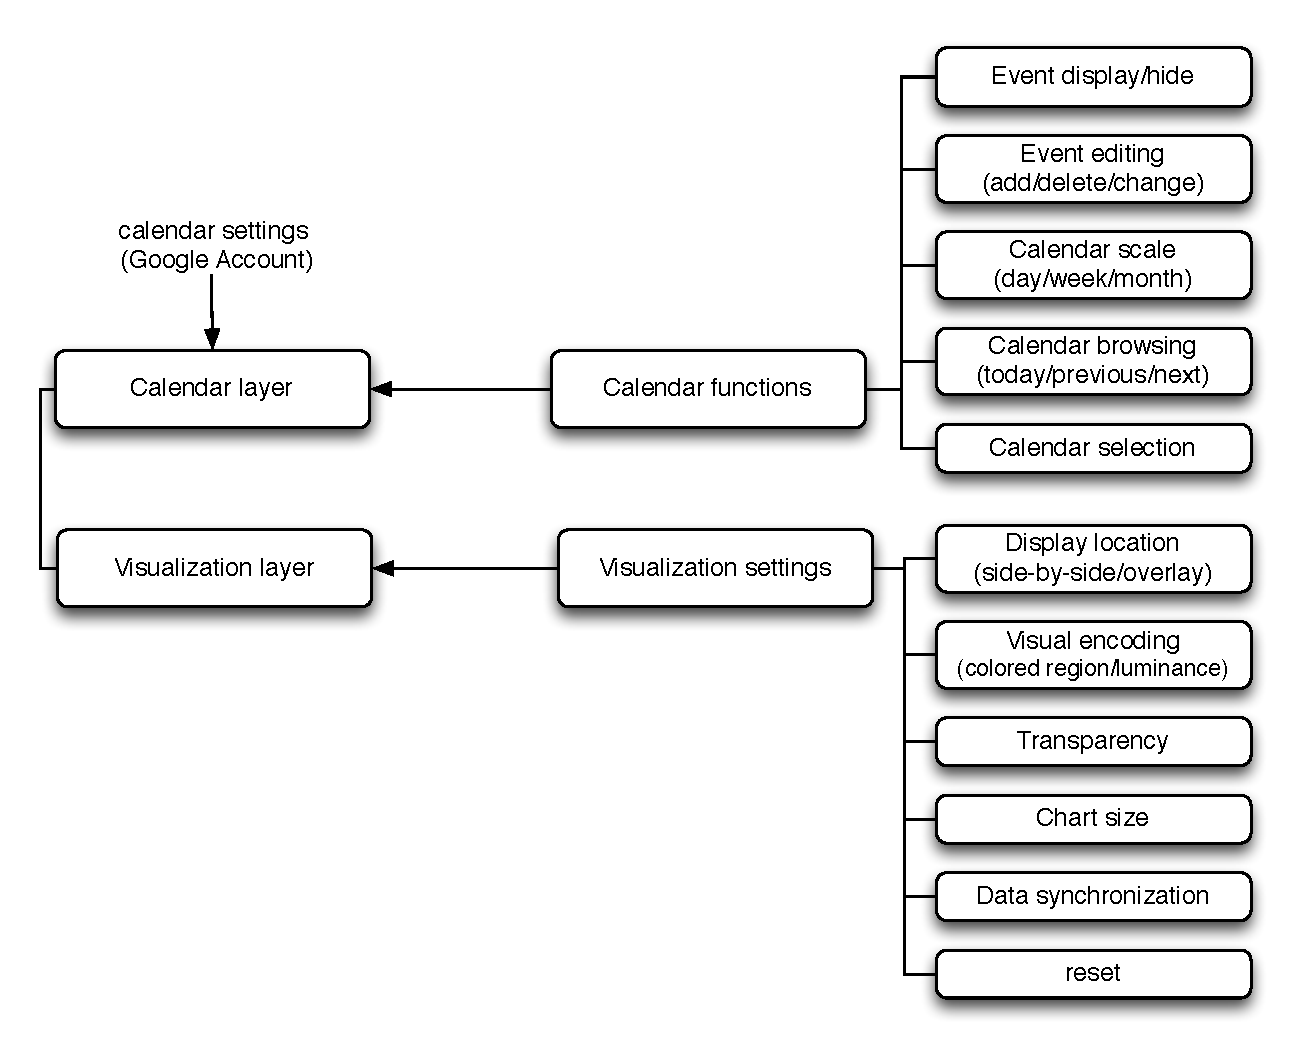
\includegraphics[width=\columnwidth]{figures/designComp}
\caption{Architecture of the on-calendar visualization system.}
\label{fig:archi}
\end{figure}

In the application, personal calendars are placed in foreground and the data visualization is displayed on the background (see the architecture in Figure \ref{fig:archi}). The calendar settings are controlled from one's google account (e.g., event colors). The on-calendar application facilitates basic calendar functions, allowing users to select calendars to display, edit their calendar events, and control the calendar view. The drop-down list from ``Select Calendar'' button enable users to select multiple calendars to display. The interactions of event editing are kept the same as Google calendar, for example, clicking event brings up pop-up dialog window for event details.

The visualization layer can be customized with the top control panel. For example, the chart can be displayed either overlapped or side by side. Users can also choose the visual encoding: either colored-region, as shown in Figure \ref{fig:implementation1}, or luminance. To balance the ambience of foreground calendar events and background data stream, the user is also allowed to adjust the settings of transparency, visualization color (with grey as default), and chart scale. Meanwhile, a script is running at backend to collection data of  user interactions, e.g., the time when the application is brought up, what buttons users click, what visualization settings users change, etc.

%%%%%%%%%%%%%%%%%%%%%%%%%%%%%%%%%%%%%%%%%%%%%%%%%%%%%%%%%%%%%%%%%%%%%%%%%%%%%%%%
%%%%%%%%%%%%%%%%%%%%%%%%%%%%%%%%%%%%%%%%%%%%%%%%%%%%%%%%%%%%%%%%%%%%%%%%%%%%%%%%
%% Chapter - pilot studies
%%%%%%%%%%%%%%%%%%%%%%%%%%%%%%%%%%%%%%%%%%%%%%%%%%%%%%%%%%%%%%%%%%%%%%%%%%%%%%%%
%%%%%%%%%%%%%%%%%%%%%%%%%%%%%%%%%%%%%%%%%%%%%%%%%%%%%%%%%%%%%%%%%%%%%%%%%%%%%%%%

\startchapter{Pilot Studies}
\label{chap:pilot studies}
In the viability study, visual interference and perceptability were investigated with ``hard-coded'' data and tasks (Chapter \ref{chap:viability study}). The implementation enables real-time data and allows users to interact with the personal data in real-life context.  Meanwhile, I needed to investigate if the implementation follows the design goal and is inline with the results in the viability study.
Thus, I conducted two case studies as pilot studies with the early version of implementation: home energy conservation (with home power meter data) and personal physical activities (with data from Fitbit), where the data are highly related to personal context (e.g., time, locations and activities).  In this chapter, I describe two case studies where I deployed the prototype tool in an experimental eco-friendly town house and with a small group of students, respectively. The cases studies were aimed to  test the early version of implementation in real life situation and identify usability issues, which helped to revise the application for later field study.  As well, I present the implementation revisions at the end of the chapter.

\section{Household Energy Consumption}
In the first case study, the web application was deployed to people living in an eco-friendly smart home \footnote{https://www.sfu.ca/westhouse.html} (see Figure \ref{fig:westhouse}) with the data source connected to their electricity meter.  This experimental townhouse was occupied by tenants, and was equipped with different sensors to collect data of various utility consumption sources.  The data feeds synchronized with the calendar tool were the overall electricity consumption for the home.  Both of the tenants were musicians, have flexible working schedules and practice at home regularly even on weekdays. In this case, the calendar tool may be helpful to reveal the pattern of their at-home activities and the relationship between their consumptional behaviors and electricity use.

\begin{figure}[h]
\centering
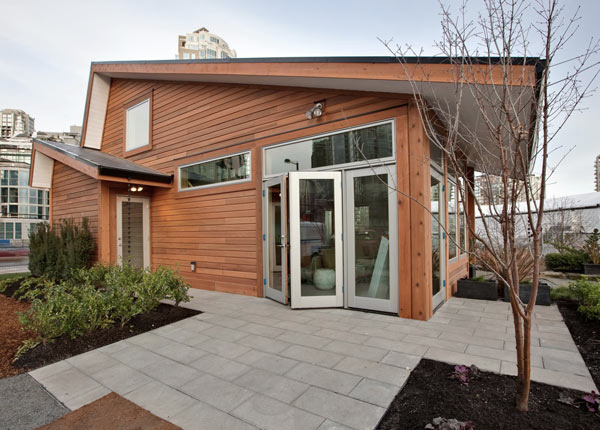
\includegraphics[width=\columnwidth]{figures/westhouse}
\caption{Westhouse: eco-friendly smart home for the case study. }
\label{fig:westhouse}
\end{figure}

The study had two phases: a baseline session and a prototype deployment session.  The first session was to understand baseline energy consumption, and did not ask the participants to use the web application.  I conducted an interview with the participants after the first session.  Afterward, the participants were introduced to the web application and asked to use the application in the way they use digital calendars in their daily lives for the next two months.  At the end of the second session I conducted another interview with the participants.  Questions in the interviews were mostly about the participants' understanding of their energy consumption behaviors, their experience of using the calendar tool in everyday life, and how they used the contextual information from personal digital calendars to make sense of their consumption data.

By the end of the study, the participants reported that the calendar events were helpful as a reference tool that helped them figure out couple of things, e.g., the baseline usage of the house, spikes caused by the fridge, the heater and the washing machine, etc. They could easily see what days they worked at home, went out because of work, went on vacation, etc. For example, the wife reported that she had noticed a continuous large consumption chunk one day in the past, and then from the calendar information (it was her concert on the next day) she figured out that it was when she was cooking a lot of food for a party after the concert. From the temporal data positioned along the timeline, she also realized that using stove took less power than oven because the using the oven usually took a longer amount of time. The participants also reported the general context provided by the calendar view helped them identify some gaps between their prior knowledge and current facts, even when the activity was not marked on the calendar. For example, they usually did laundry right after they got up. The spikes caused by the spinning of the washing machine in the beginning phase were totally out of their expectation (``I am surprised to see the spinning takes so much power.''). However, the on-calendar visualization tool saw low usage after the first two weeks. The participants reported that they were more familiar with iCal more than Google calendar, and used iCal more often. The inconsistent look and features prevented them using the on-calendar visualization as the daily default option. They hoped that the visualization could be integrated into their iCal application. Thus, I modified the design of the application and make the look and features more close to Google calendar and also refined the recruiting requirements in the later field study where participants who were familiar with Google calendar were included (Chapter \ref{field:screening}).

\section{Personal Fitness}
In the second case study, we deployed our calendar application to 10 undergraduate students as part of a Psychology seminar course.  In contrast to the energy consumption case where the consumption is related to activities of all family members, I considered the fitness case because personal fitness data might be more relavent to individuals' activities and was directly linked to one's personal calendar.

\begin{figure}[h]
\centering
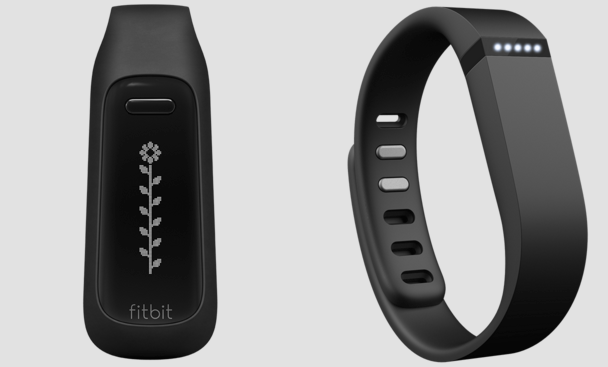
\includegraphics[width=\columnwidth/2]{figures/fitbit_tracker}
\caption{Fitbit trackers use in case study of personal fitness }
\label{fig:fitbit}
\end{figure}

Participants (eight females and two males) in this study were undergraduate students from the Psychology department with age between 21 and 25. They were provided Fitbit devices \ref{fig:fitbit} (all of them were novice Fitbit users), with which they were asked to track their daily physical activities. However, online Fitbit accounts were not provided, so they could not use the default Fitbit online tool for feedback purposes. Instead, they could only use the display on the device for feedback information. The study lasted for 4 weeks. In the first two weeks, they could only rely on the device display for feedback, and the on-calendar web application were introduced after the first two weeks. In the latter two weeks, they were asked to use the on-calendar application as the default feedback tool. Two interviews were conducted at the end of week 2 and week 4, respectively. In the first interview, participants were asked about their experience in the first two weeks. I also helped participants set up the device and gave them a tutorial. In the second interview, participants were asked about their experience of using the on-calendar application and how they use the calendar context for reasoning. (see outlines in Appendix \ref{}).

Participants in this study reported that they liked the idea of integrating Fitbit data into a digital calendar. It helped to reveal their school-life patterns, for example, the start of the day, that they were sitting most of the time for classes, that they walked (or ran) during class intervals, and that they studied during the weekend. It also helped to easily identify anomalies. For example, a participant found his active activities mostly happened at midnight. It is because he often worked in a restaurant with a night shift. The on-calendar visualization also revealed errors in data collection. One participant found the movement during her class event on her calendar, and suspected it was her hand movement even when she was sitting. Participants' comments about visualization preferences confirmed with the lab results in early viability experiments. They reported that colored region was easier to perceive than luminance (``I can see the time, where the peaks are, and the intensity''). Visualization display overlapped (``in-cell'' option) was regarded as easier to read because the chart was bigger, even though overlapped with calendar events.

However, part of participants' Fitbit data was often found missing on the visualization. They reported in the interview that they forgot to wear the device or charge the battery. The novice Fitbit users may not be familiar of using the devices or not comfortable to wear the device all the time. Thus in the later deployment, experienced Fitbit users were recruited (Section \ref{field:screening}).

Most of the participants in this study had very sparse calendar events because the calendar events on students' calendar were very simple, mostly related to their school schedules (for example, course arrangement). The only exception was one participant who has busy calendar schedules (because he had to manage a few student organizations) and used digital calendar very frequently. During the study he used the on-calendar visualization more than the others. I suspect this might be a factor to influence the application usage in this case, so I tried to balance the diversity of participants in the later field study (Section \ref{field:screening}).

Meanwhile, the same issue as the first case study was brought up as well. The overall usage of the on-calendar application was very low. Participants commented on the inconsistent look\&feel and features compared with calendar tools that they used most often. Some participants suggested to include the visualization in their iCal application. Thus, a revision of the on-calendar visualization seemed necessary.

\section{Summary of Pilot Studies}
These pilot studies were aimed to collect feedback on the design approach and identify usability issues with our early version of implementation. Overall, the results were encouraging. Participants liked the concept of integrating a data stream within a personal digital calendar. They believed it was an easy way to access and keep track of relevant data. They also found that the context provided by their calendars was helpful for interpreting patterns and abnormalities in the data. More interestingly, we found that people could easily see their life routines reflected in the on-calendar visualization, even though many of the relevant routine activities were not recorded in the calendar (e.g., cooking, laundry, showers, etc.). This suggests that the context from personal calendars can provide high-level information to help people understand personal data patterns without requiring extra effort for people to record their daily routine activities.

Meanwhile, the studies also revealed a few usability issues with the application. The logging scripts showed that the online web application had very low usage after the first few days when it was introduced, which might have been caused by some inconsistencies in functionality and look \& feel as compared to the commercial calendars that participants regularly used (e.g., iCal or Google Calendar). These inconsistencies presented a barrier for participants and prevented them from routinely using the web application instead of the one they currently use. This meant that this tool was used more as a dedicated visualization tool for accessing the data stream rather than the way as intended, where the data would be viewed in a secondary background stream. However, participants hoped the additional visualization layer could be added into their own calendar application, showing merit for the intended design. These results suggest that the prototype needed to be revised before larger scale deployment, to make the features consistent with digital calendars that people use regularly.
Moreover, I found that visualization customization and time scales may be subject to many personal preferences. Some preferred week view for bigger charts, and some preferred month view for overview. Participants reported that the advantages of colored-region was that the spikes helped her recall things for reasoning. However, luminance displayed in-cell seemed to be most irritating for them. For these reasons I kept the visualization settings user-adjustable.

\section{Design revision}
The revision of early version of implementation primarily focused on the consistency of functions and look \& feel with exiting calendar tools (specifically, Google Calendar in this case). The final version was implemented with PHP and JavaScript (D3.js for visualization layer), together with Fitbit API \footnote{https://dev.fitbit.com/} and Google Calendar API \footnote{https://developers.google.com/google-apps/calendar/}  (see Figure \ref{fig:implementation2}).

\begin{figure}[h]
\centering
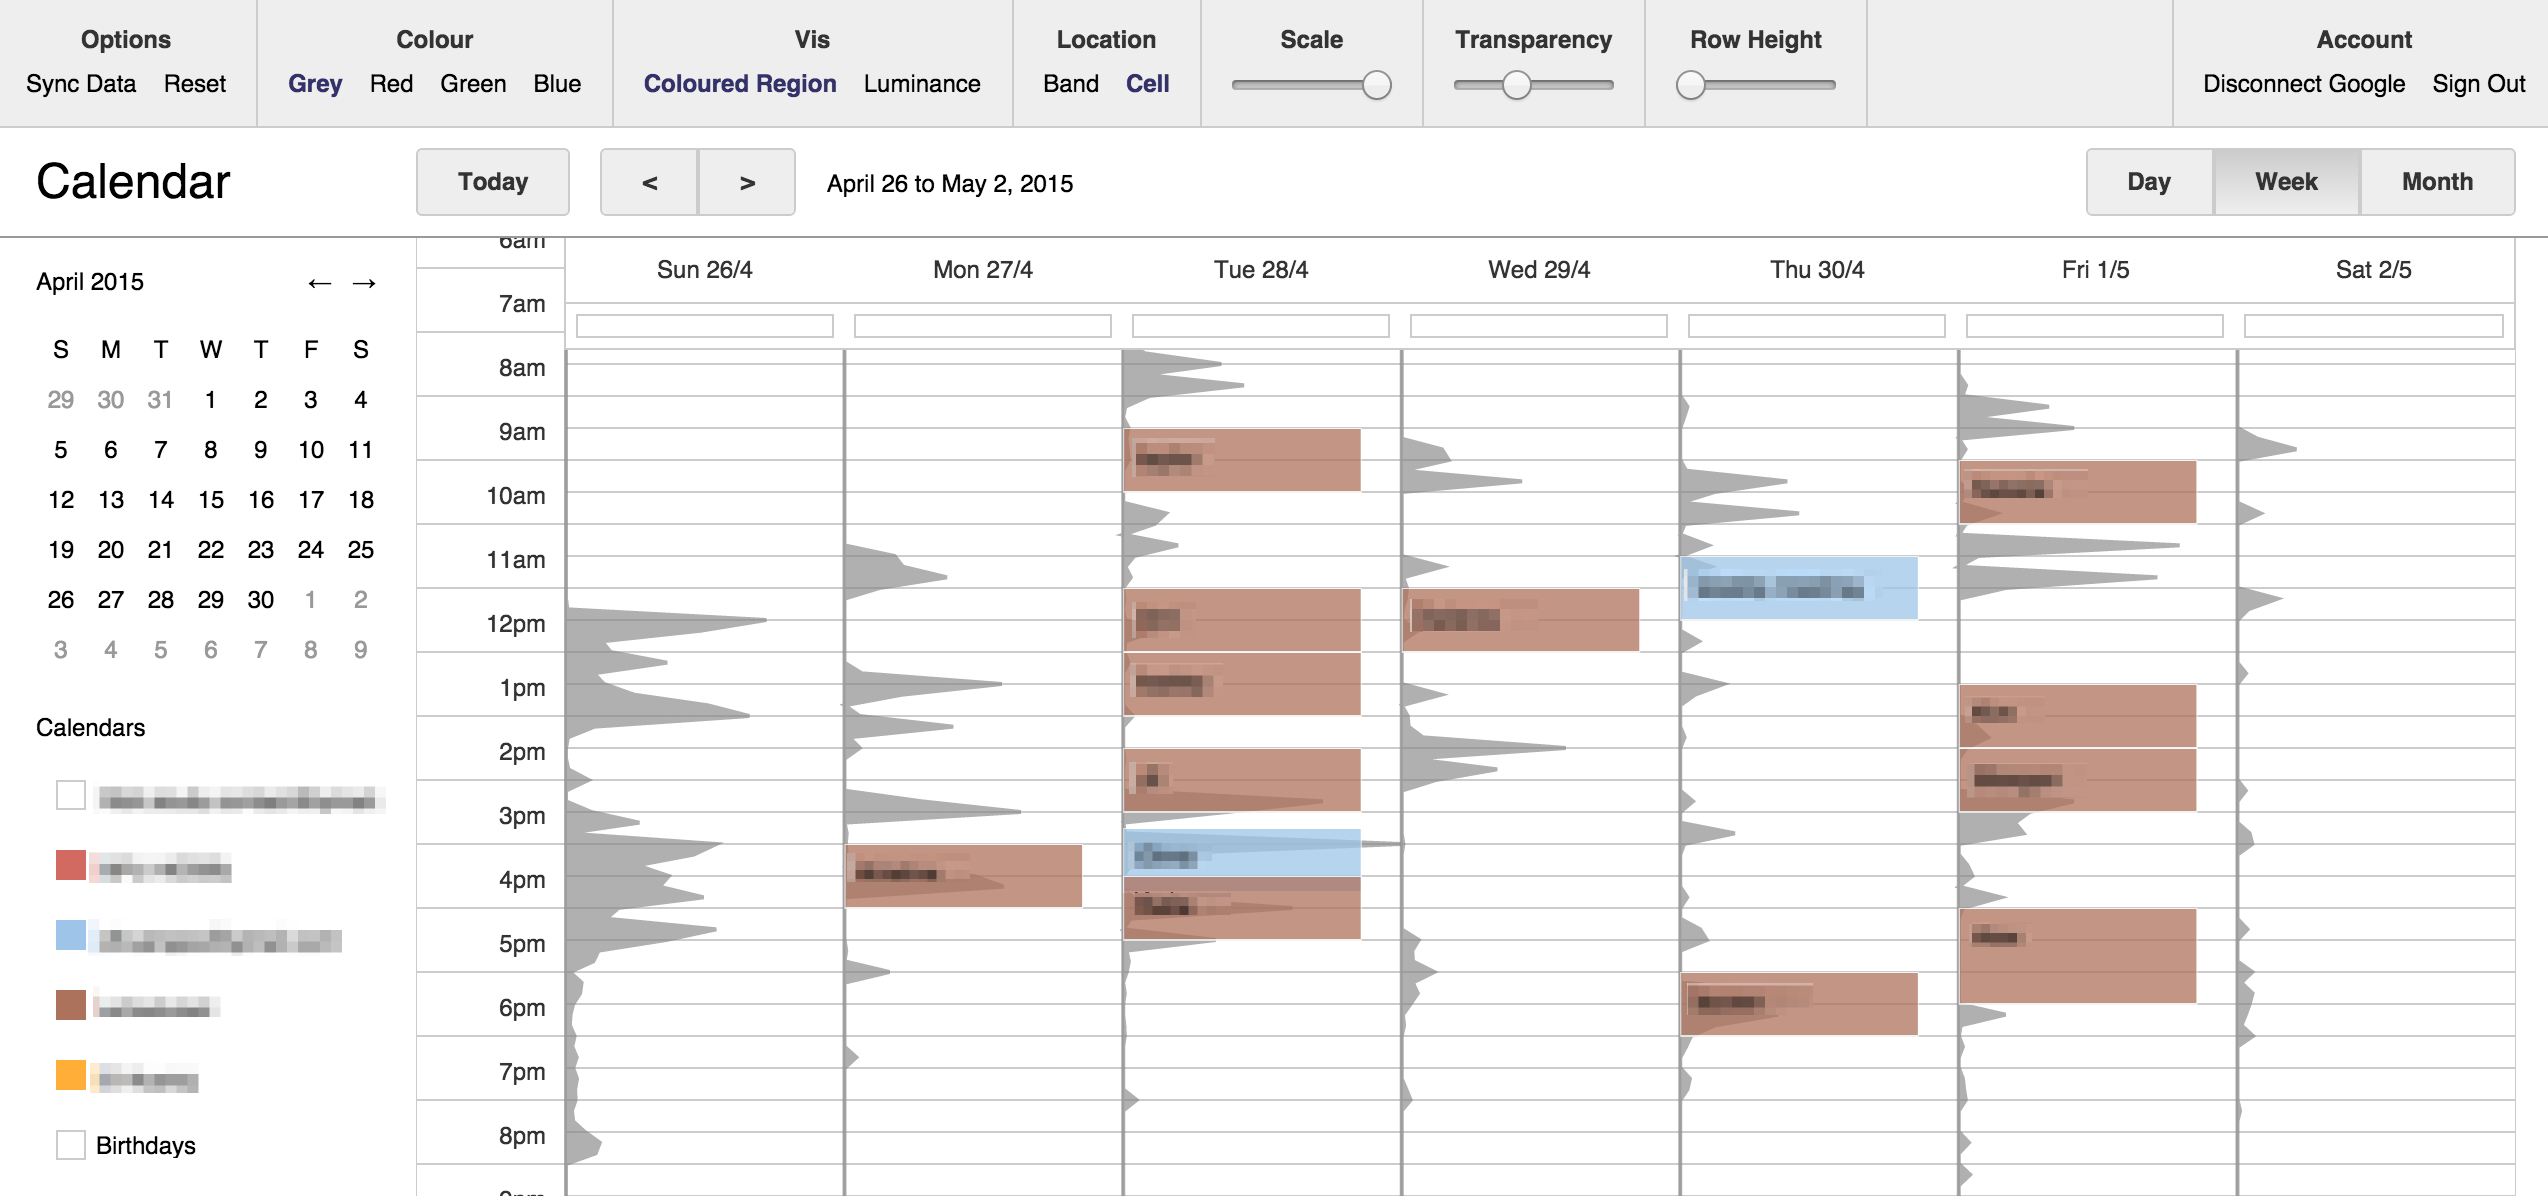
\includegraphics[width=\columnwidth]{figures/implementation2}
\caption{On-calendar feedback application used in the study (week view with Fitbit data displayed as a line graph overlapped with calendar events). See more screenshots in Appendix \ref{}. }
\label{fig:implementation2}
\end{figure}

First, to make the application easy to manage, previous customized visualization settings are remembered for each individual. People could customize the visualization to fit themselves, and the on-calendar visualization was set with their previous preference the next time they log in.

The on-calendar application was expected to be used as everyday calendar tool, so I made the control panel (for adjusting visualization settings) more subtle and put it at the top.  This was to reduce the distraction of non-calendar functions while people are performing scheduling tasks.

The calendar layout was re-designed according to the Google Calendar \footnote{https://calendar.google.com/calendar} layout. Calendar browsing buttons (e.g., selecting time scale) were placed on the top of the main calendar view. A small calendar was added on the left for quick date selection. Below that was the calendar selection panel, with which people could decide which calendars to be displayed in the calendar view. Similar as in Google calendar, all day events could be shown at the top of the day below the date label (only in day view and week view).

Other than that, people were allowed to customize the row height of calendar cells. With smaller height, a longer time period of the day can be seen (only in day view and week view), in order to provide a better overview. In the consideration of privacy, functions of access control were enabled (e.g., automatic sign out of the user from the application)


%%%%%%%%%%%%%%%%%%%%%%%%%%%%%%%%%%%%%%%%%%%%%%%%%%%%%%%%%%%%%%%%%%%%%%%%%%%%%%%%
%%%%%%%%%%%%%%%%%%%%%%%%%%%%%%%%%%%%%%%%%%%%%%%%%%%%%%%%%%%%%%%%%%%%%%%%%%%%%%%%
%% Chapter - Field study
%%%%%%%%%%%%%%%%%%%%%%%%%%%%%%%%%%%%%%%%%%%%%%%%%%%%%%%%%%%%%%%%%%%%%%%%%%%%%%%%
%%%%%%%%%%%%%%%%%%%%%%%%%%%%%%%%%%%%%%%%%%%%%%%%%%%%%%%%%%%%%%%%%%%%%%%%%%%%%%%%

\startchapter{Field Study}
\label{chap:field study}
Results from pilot studies confirmed that the on-calendar design could provide daily life context for people to reason about their data and support ambient attention. However, insights from pilot studies are limited. The early implementations had a few usability issues. Participants in the pilot study may not properly represent the target user as expected. After revising the application based on the feedback, I deployed it in a longitudinal field study. In this chapter, I describe an eight-week field study with the latest implementation connected to Fitbit data. This study primarily focuses on two questions: 
\begin{itemize}
	\item{To what extent can people use calendar data as context for reasoning about their fitness data?}
	\item{How do people react to the idea of integrating feedback data into their personal calendars?}
\end{itemize}

This study compared experimental and control groups (who used our calendar prototype and Fitbit's standard feedback tools respectively), aimed to investigate mash-up design approach and the influence of providing extra context for reasoning. The emphasis was on exploring people's experiences with the on-calendar visualizations rather than measuring differences in behavior change, as suggested by early research \cite{strengers_designing_2011,pierce_consideration_2010,costanza_understanding_2012, klasnja_how_2011}. Therefore, I employed a qualitative approach with open-ended research questions rather than statistical comparisons between the groups.
% rational of method choice?

\section{Participants}
\label{field:screening}
I recruited participants among existing Fitbit users instead of providing Fitbit devices, considering that existing users, compared with new users, already had some motivation to use feedback tools. Existing users were also already experienced with Fitbit's basic feedback applications, and for them, using a fitness tracker and its software would not itself be a novelty. Meanwhile, the participant screening required that participants be familiar with digital calendars and have a Google account (necessary to use the web application). In total, 21 Fitbit users participated in this study with age ranging from 20 to 60+, 15 female and 6 male (see Table \ref{table:participants}). Two of them (one female and one male) dropped out after the first two weeks. Seven of them used other fitness trackers before.

\begin{table} 
\begin{center}
\begin{tabular}{|r|c|l|l|c|}
\hline
 Participants   &  Age Group  &  Gender   & Fitbit experience  &   number of fitness   \\
  & & & (current tracker) & trackers used  \\
  & & & & before current one\\
 \hline
p1	& 30-39	& Male	& 2.5 years	& 0 \\
p2	& 18-29	& Female	& 1 month 	& 0 \\
p3	& 30-39	& male	& 1 year and 1 month	& 0 \\
p4	& 30-39	& Female	& 3 months	& 0 \\
p5	& 18-29	& Female	& 3 months 	& 0 \\
p6	& 40-49	& Female	& 11 months	& 2 \\
p7	& 18-29	& Male	& 2 Months	& 0 \\ 
p8	& 30-39	& Female	& 1 year and 1 month	& 2 \\
p9	& 60+	& Female	& 2.5 months	& 2 \\
p10	& 18-29	& Female	& 3 months	& 0 \\
p11	& 40-49	& Female	& 4 months	& 0 \\
p12	& 18-29	& Female	& 1 year	& 2 \\
p13	& 18-29	& Female	& 1 month	& 2 \\ 
p14	& 30-39	& Male	& 1.5 years	& 0 \\
p15	& 30-39	& Female	& 4 months	& 0 \\
p16	& 60+	& Female	& 1 year	& 2 \\
p17	& 30-39	& Female	& 4 months	& 0 \\
p18	& 30-39	& Female	& 3 months	& 0 \\
p19	& 30-39	& Male	& 3 weeks	& 2\\
\hline
%\multicolumn{4}{l}{\textsuperscript{*}\footnotesize{Significant difference compared with the control condition}}
\end{tabular}
\caption{participants in Fitbit field study}
\label{table:participants}

\end{center}
\end{table}
%% need to adjust the participant ID

\section {Conditions}
Participants were randomly divided into two groups: Control (C1$\sim$C9) and Experiment (calendar Visualization) (V1 $\sim$ V10). This design allowed us to investigate whether extra context from a personal calendar could improve people's understanding of their feedback data. Participants in the control group used their baseline feedback application (i.e., that provided by Fitbit). Participants in the Visualization group used the baseline feedback application in the first two weeks; they were then introduced to our web-based calendar visualization after week 2. Visualization group participants were asked to use our calendar application as their primary scheduling and feedback tool; however, they were not prevented from also using their default calendar service (e.g., Google calendar or iCal) and Fitbit's feedback tools. With the control condition, the use of original Fitbit application is equal in the two groups.

\begin{figure}[h]
\centering
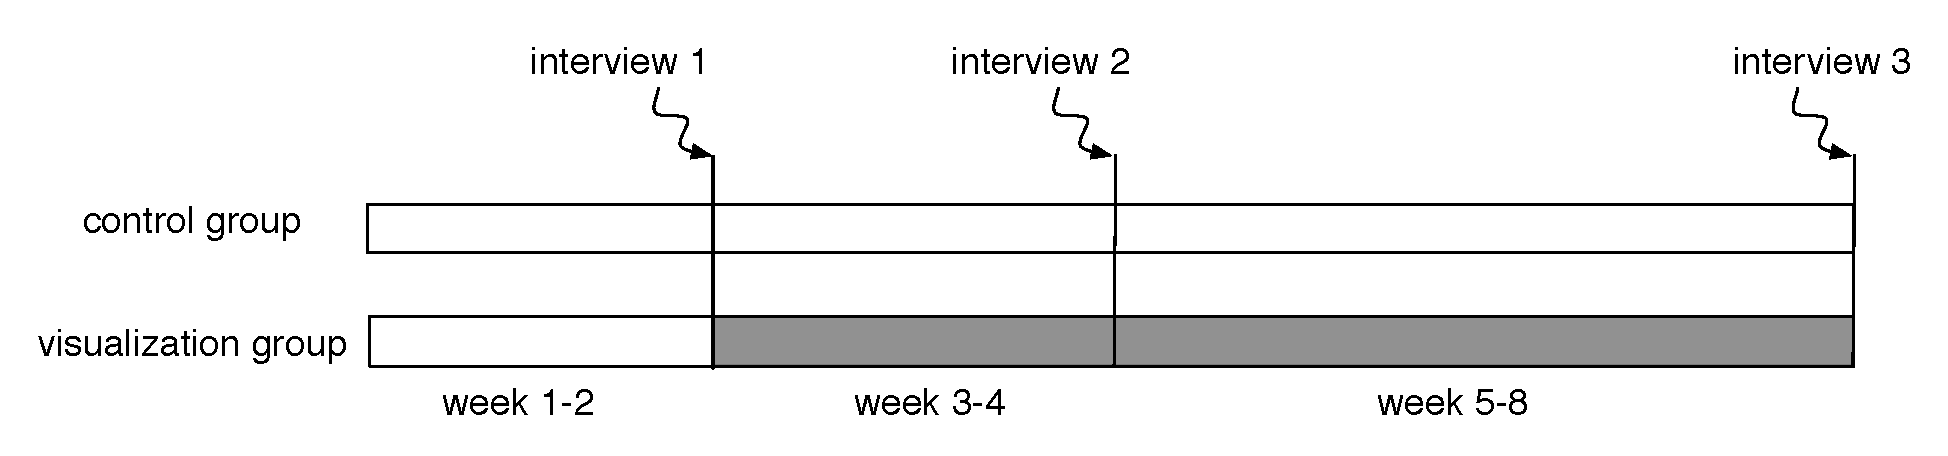
\includegraphics[width=\columnwidth]{figures/studydesign}
\caption{Study procedure }
\label{fig:studydesign}
\end{figure}


\section {Procedure}
Before the first week, we met participants and introduced the procedure. During the first two weeks baseline information was collected and participants were told to continue using Fitbit as they had done in the past (see Figure \ref{fig:studydesign}). I interviewed all participants in week 3, during which Visualization group participants were introduced to our on-calendar visualization.This interview was to investigate how the participants use their feedback tools currently, and set up the baseline of using feedback tool for reasoning to compare before and after the visualization tool was introduced to Visualization group. 
To investigate their initial experience and help the participants on the technical issues of using on-calendar feedback application, I interviewed all participants again in week 5. Participants in the Control group were also interviewed to balance the influence of interview intervention in the Visualization group.
 Final interviews were scheduled in week 9, in which participants shared their experience of using the feedback tool in everyday life during the study. 
 During these interviews, participants were asked to review their Fitbit data with and without their feedback application, identify patterns and anomalies, and reason about the patterns and anomalies. These tasks were to investigate the general awareness of personal awareness, how they reason about data patterns and anomalies using feedback tools, and how they use inferential context in the reflection. 
 Meanwhile, during the total eight weeks, participants were asked to fill in a weekly International Physical Activity Questionnaire (IPAQ) \cite{ipaq} through an online portal. Reminder emails with the survey link were sent to them on Friday afternoon every week. At the end of the final interview, participants in the control group were also introduced to the on-calendar application and asked for comments. The interview outlines are included in Appendix \ref{}.



\section{Data collection}
The data collection included weekly surveys, application logs and interviews. Although participants’ Fitbit data were accessible to measure physical activity level, this data was not to used  because of its incompleteness. (Fitbit cannot accurately capture activities such as cycling, spin class, and swimming.  In addition, Fitbit devices occasionally malfunctioning.)  Instead, the estimated physical activity (PA) were evaluated by the weekly IPAQ survey that is often used method to measure physical activities \cite{ahtinen_user_2009, consolvo_design_2006, biernat_assessment_2008,harrison_activity_2015,charbonneau_teach_2011,du_efficacy_2014}.  V8's survey data were dropped from the analysis because only 3 surveys were submitted. The remaining 18 participants submitted at least 6 entries of the online survey. 

Metabolic Equivalent (MET) is a commonly used physiological measure to assess physical activities \cite{jette_metabolic_1990}. METs of the weekly surveys were calculated according to the scoring protocol of IPAQ \cite{ipaq}. Meanwhile, interactions of participants while using the calendar visualization (e.g., change visual encoding or layout) were automatically logged. In the interview , the participants were asked to recall their PAs to explain their data patterns, their experience using the feedback tools, and the impact in their life. During the interview, they were also asked to bring up their feedback application and reason about their own data patterns. I observed how they interacted with the application and how they performed tasks to reason about their data.
The following analysis focused on qualitative feedback about the on-calendar design approach. This study was most interested in how the approach would influence people's ability to reason about their feedback data, and to what extent they would find the on-calendar visualizations helpful and/or disruptive. Therefore, I employed a primarily qualitative analysis approach.


%{fitbit data}
\section {Results}
\subsection{Physical activity levels}
I first examined the physical activity (PA) variation of the two groups before and after the calendar intervention. The results showed the two groups were not significantly different in MET measures (t(16) =0.53, p=0.60, Cohen\rq d=0.27). PA tended to increase more for the experimental group than for the control group, but this was overshadowed by individual differences (Figure \ref{fig:mets}). Participant comments suggested that behavior change (PA variation) was most influenced by other aspects in their lives, e.g., traveling (V2, V6, C5), relocation (V10, C6), facility service interruption (C3), or a training program (V5, C4). However, the influence of single intervention is difficult to qualify in behavior change and measuring behavior change was not the main goal of this study.
Instead, I focused the majority of our analysis instead on system use, its role in the feedback process, and how it influenced people's reasoning.

\begin{figure}[h]
\centering
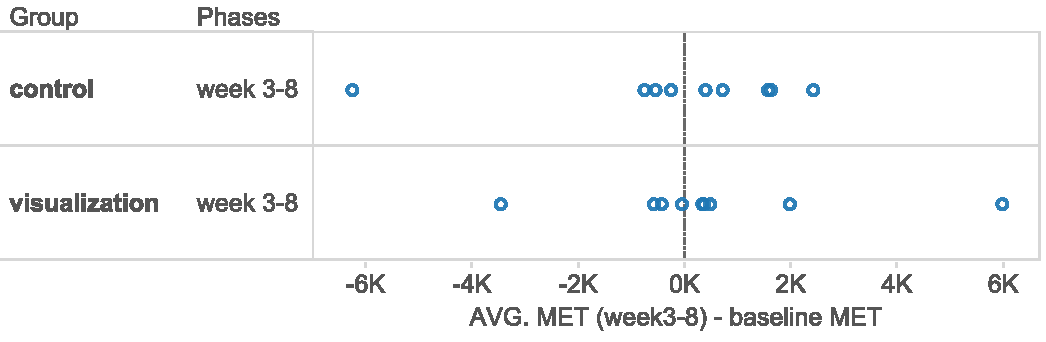
\includegraphics[width=\columnwidth]{figures/avgMET}
\caption{Change in MET values from weeks 1-2 (baseline) to weeks 3-8 (intervention) for individuals in control and experiment groups. Each mark represents one participant’s change in average MET scores. }
\label{fig:mets}
\end{figure}

\subsection{System Use}
Application logs showed 152 visits (user sessions) and 208 user interactions (setting and view changes) during the study. The peak usage was in the morning (around 10am) and in the evening (around 9pm). The application remained active for durations ranging from one minute to four days (M = 1043, SD = 2791), indicating that people used the application quite differently: some brought it up for a quick look while others continually kept the tab open. That means participants might keep the browser tab of the application open for calendar use while working with their computer. This might indicate the efficiency of the mash-up design approach: which is to use an additional visualization layer to support attentional ambience. 

\begin{figure}[h]
\centering
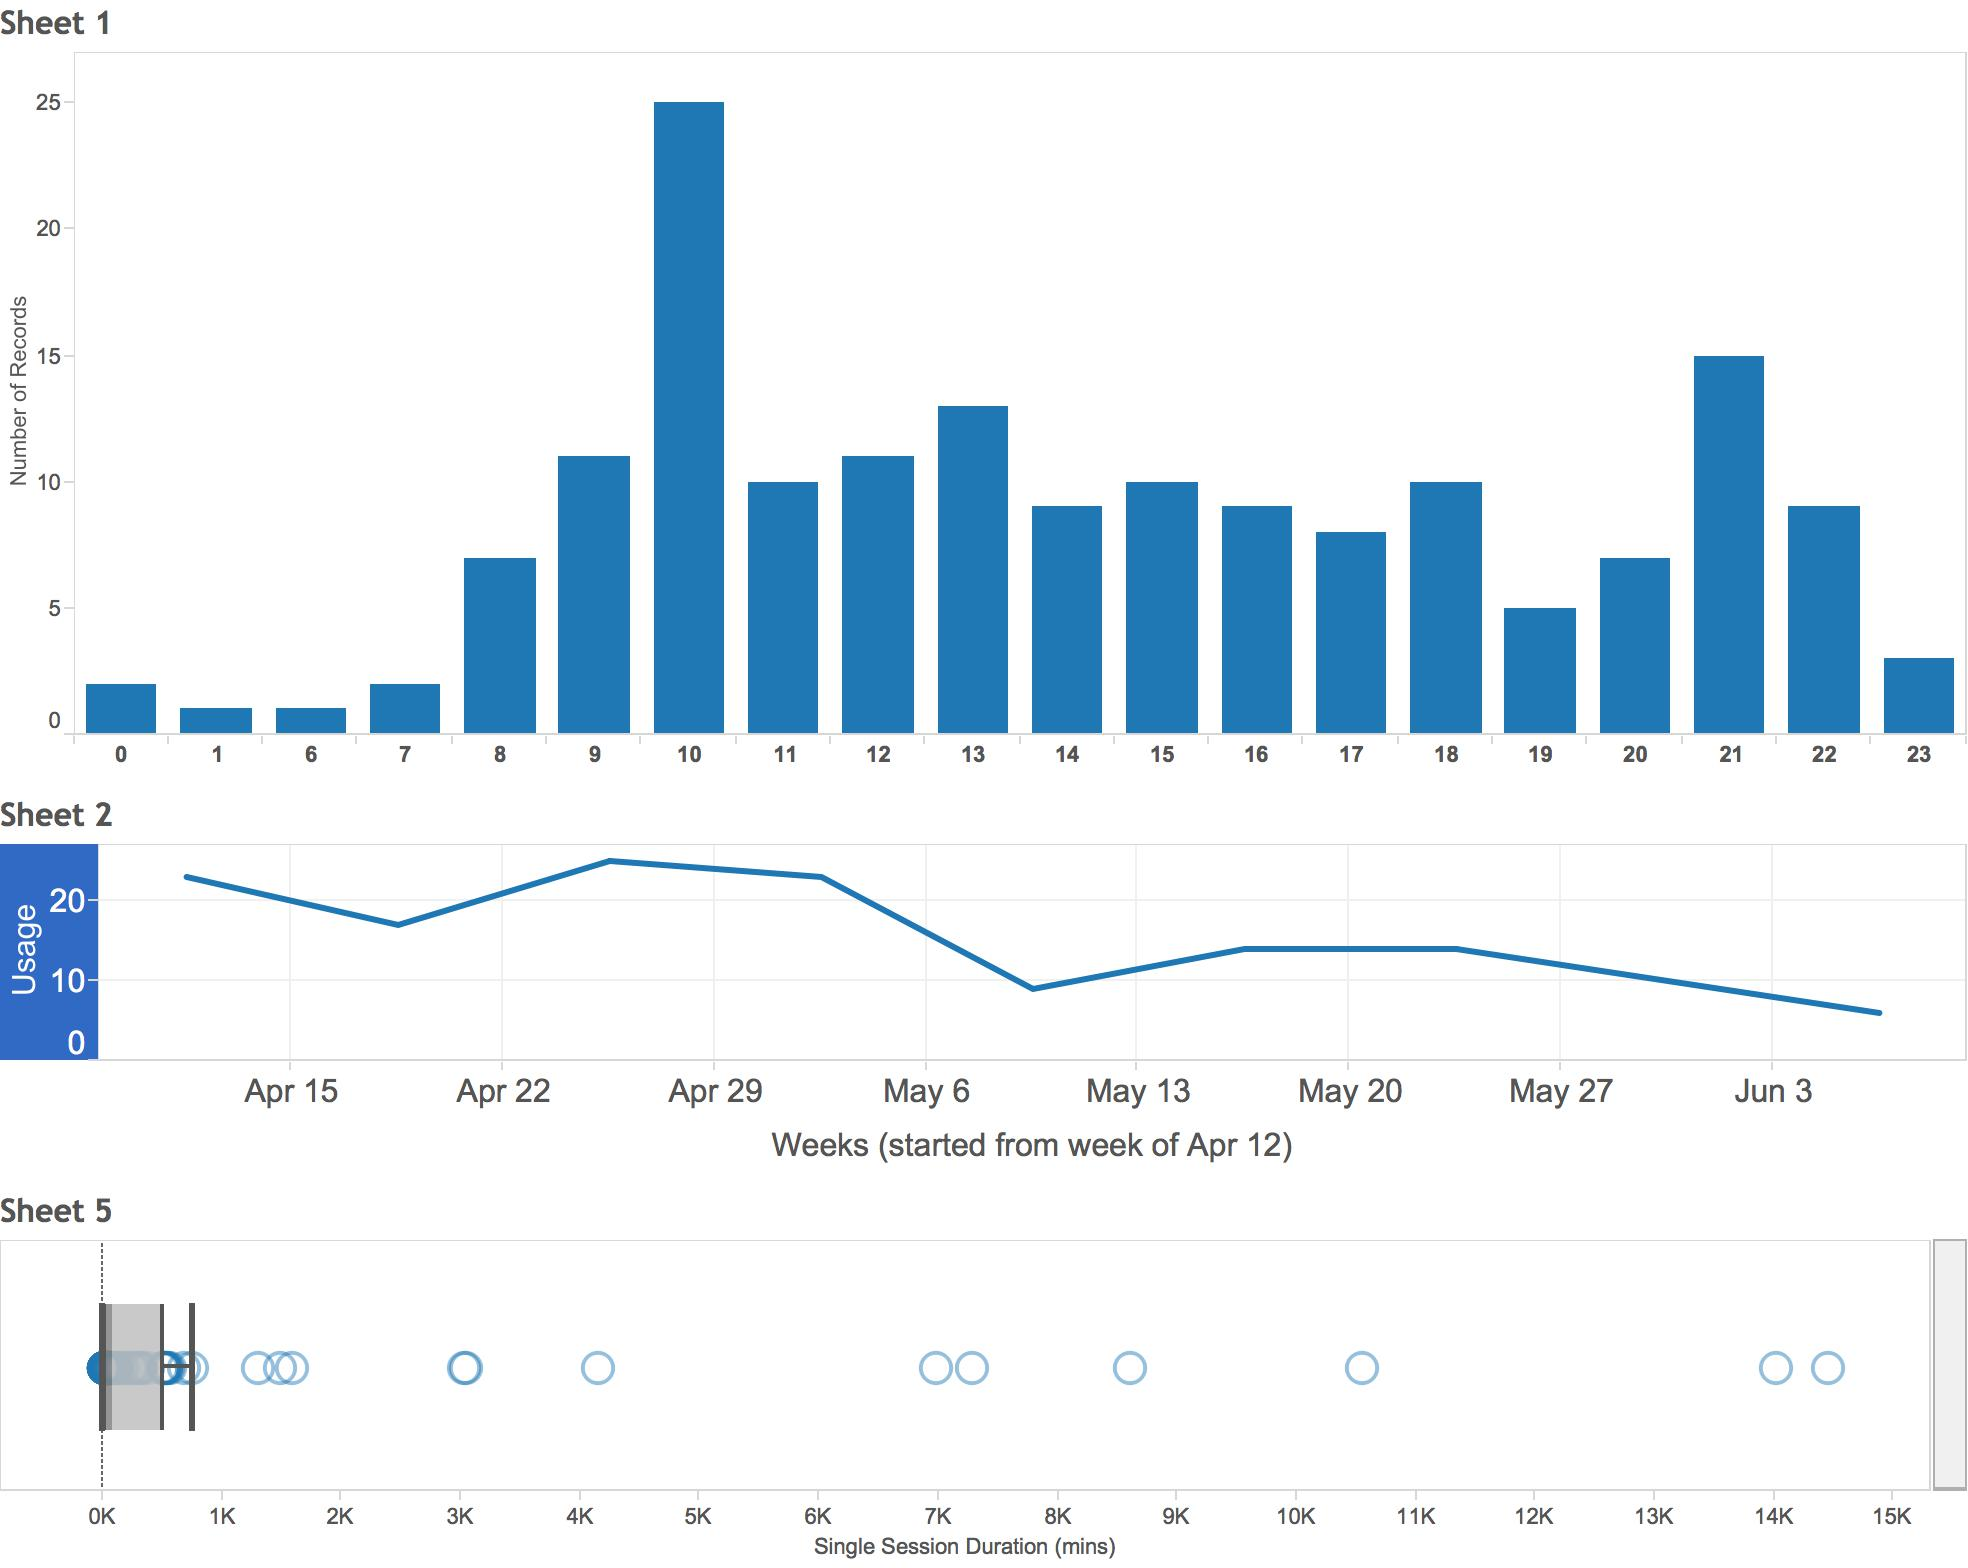
\includegraphics[width=\columnwidth]{figures/usage}
\caption{Change in MET values from weeks 1-2 (baseline) to weeks 3-8 (intervention) for individuals in control and experiment groups. Each mark represents one participant’s change in average MET scores. }
\label{fig:system_use}
\end{figure}

By default the visualization was encoded with Colored Region and in grey color (with 60\% transparency), and displayed with an overlapped layout in the week view.  When the application was introduced, participants were asked to try and explore all possible settings. The application was implemented so that it could remember customized settings, so the bias of default visualization settings was minimized. Application logs (Figure \ref{fig:log}) also showed that all participants preferred Colored Region (line graphs) as the visualization setting. They reported that luminance as the visual encoding required extra cognitive effort to understand, and that color made the calendar look busy and interfered with calendar events (particularly when the calendar events were color coded). Grey color and overlapped display were used most often, suggesting that they were least disruptive. Only one participant chose to show the visualization layer in a separate band side-by-side with calendar events (kim). In the interviews, participants also reported that the visualization layer did not interfere with their use of calendar events (V1, V2, V9, V10), especially with the grey color. This suggests that with proper visual encoding, displaying data as an additional layer on a calendar need not interfere with regular calendar use. Most participants stayed on the week view most of the time, and switched between week and month views (175 view switches were logged among 10 participants) when they explored data patterns with different time ranges and levels of detail.

\begin{figure}[h]
\centering
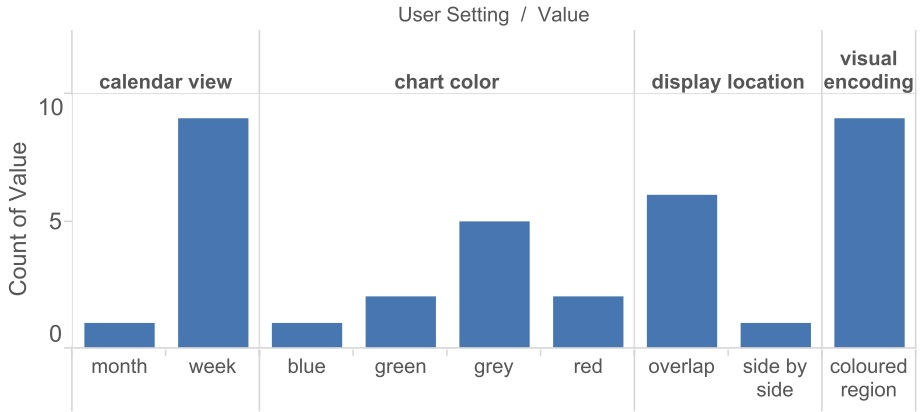
\includegraphics[width=\columnwidth]{figures/log}
\caption{Preferred visualization settings (experiment group). The most popular visual encoding was a grey line chart overlapped with the calendar data in week view.}
\label{fig:log}
\end{figure}

%visualization settings, color, transparency, view

\subsection{A Model of the Behavior Feedback Process}
I transcribed the interview recordings and conducted content analysis \cite{miles_qualitative_2013}. The coding process was facilitated by AQUAD (version: 7.4.1.2) \cite{aquad}.  First, the transcripts were open coded with a focus on how feedback tools influence understanding and reasoning about physical activity, what context the participants used for reasoning, interaction with visualization tools, how this understanding relates to one's goals and to changes in behavior, and barriers of current feedback use (example of coding??). These codes were then clustered and organized into categories of state (current physical activity status), goal (personal objectives for using feedback tools), reasoning (how one makes sense of data patterns), insights and awareness (people's understanding of their PA), behavior choice (choices about when and how to engage in physical activity) and emotion (what emotion could be evoked in the process). We then used the data to build an understanding of relationships between these concepts. This analysis resulted in the behavior feedback model illustrated in Figure \ref{fig:model}.

\begin{figure}[h]
\centering
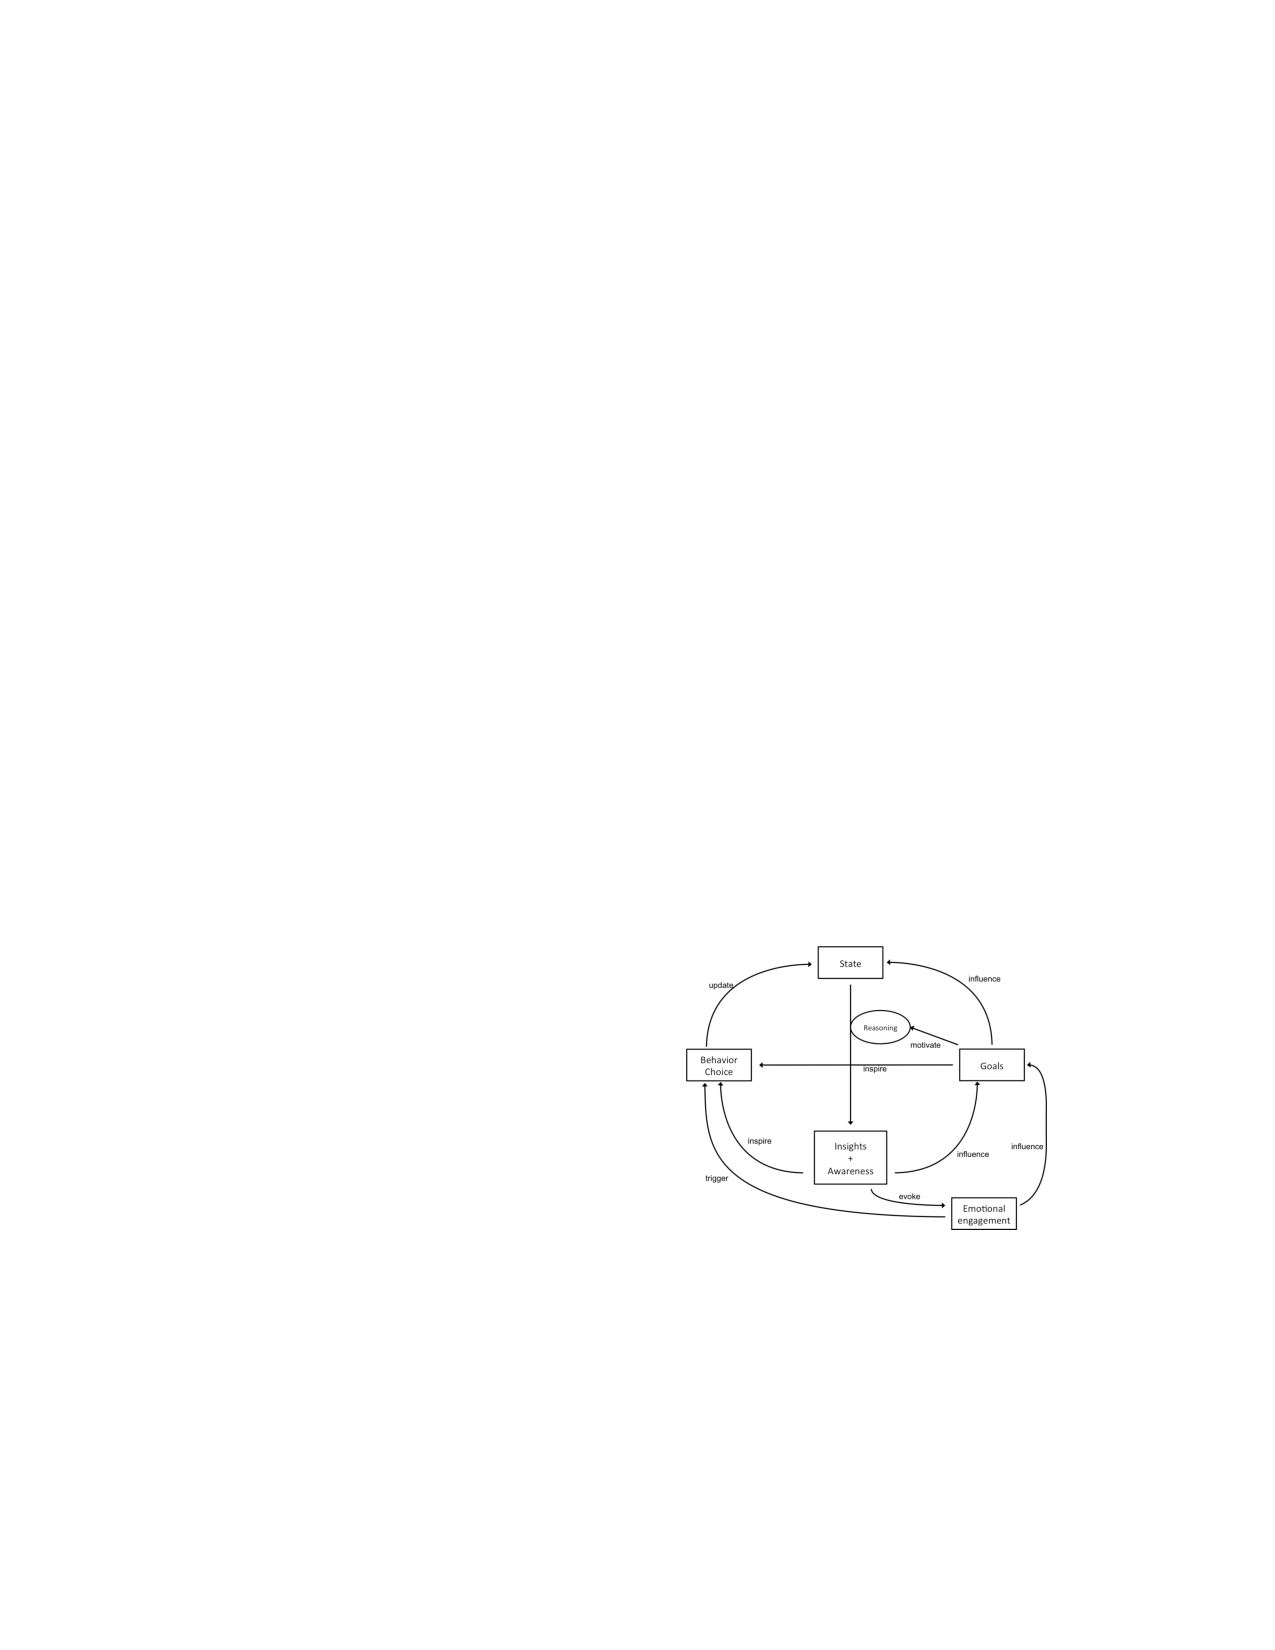
\includegraphics[width=\columnwidth]{figures/model}
\caption{Model of behavior feedback process. }
\label{fig:model}
\end{figure}

\textbf{State} represents data with respect to current status that is collected and visualized with feedback tools; for example, the current activity level, progress during the day or the week, PA routines and change. Participants reported various data about state that they would read from feedback tools, including immediate measures in the moment (e.g., active minutes, heart rate, steps) and reflective progress measures (e.g., long-term trend, activity performance, calorie balance, daily and weekly progress towards goals, and sleep quality). Participants used both data summaries and detail views to access this information.

Personal \textbf{goals} could be short-term or long-term. As an example of a long-term goal, V7 used Fitbit feedback to motivate himself to build regular gym routines that could fit in his current schedule. On the other hand, V6 used the feedback tool to track short-term daily and weekly step goals. Personal goals strongly influenced what participants expected to see about their state. V2 had to manage a health condition, so he focused mostly on sleep quality and resting heart rate. C8, who already had a regular exercise routine, mostly used feedback tools to track her exercise plan (two runs and two gym visits per week). In some cases, goals also influenced data collection. V9, hoping to know the impact of depression on his productivity, set up a daily self-report system to track his mood. V8 replaced her Fitbit device with a different model because she wanted to monitor her cardio status while exercising, a feature that was not possible with the first model.

Goals varied widely across our participants. Examples included progress checking (checking daily or weekly progress), in-the-moment monitoring (monitoring heart rate in cardio zone), exploration (exploring what exercise fits better), problem investigation (investigating sleep quality), or medical/physical condition management (managing diabetes). One's goal may vary with age as well. For example, an older participant stated, 
\begin{quote} 
``Fat burn, you can get how often I am doing, hitting the cardio level ... If I was younger that might be important. I think that probably for older people using the Fitbit, that probably the most important tool is to see that the improvement is there on a daily basis.'' (V6)
\end{quote}

Personal goals motivate people to look at their data to gain \textbf{awareness}, and to \textbf{reason} about their data to gain \textbf{insights}, by posing and answering questions. I categorized three types of questions: (1) \textit{What} (``What is the current status or performance?'', ``Do the data accurately reflect my situation?'', ``Have I done 3 runs this week?'', ``What are the data patterns in a year/month/week/day?''), (2) \textit{Why} (``Why do I have a trend like this?'', ``Why is the pattern on Friday night different?'', ``Why do I always see a spike in my data early in the morning?''), and (3) \textit{How} (``How can I improve?'', ``How can I fit running into this weeks schedule?'', ``How can I customize my exercise goals?''). 

People performed a variety of tasks to seek answers to these questions. These tasks included making comparisons, mapping Fitbit data to calendar events, integrating data, looking up items, changing the timeline scale, counting, identifying regular patterns, identifying anomalies, observing overall trends, searching related domain knowledge, and exploring what-if experiments. (table of examples) During the interviews, participants were asked to reason about their Fitbit data patterns, e.g., peak values, repeated patterns, or anomalies. The tasks they performed most often were \textit{comparisons} (19 out of 19 participants) and \textit{activity mapping} (19 out of 19 participants), in which people related data patterns to activities that happened during the same time slot. Participants also \textit{compared their progress} with their goals (18 out of 19 participants) or \textit{baselines} (3 out of 19 participants), with the \textit{historical performance}(3 out of 19 participants), or with \textit{others} (8 out of 19 participants). By relating their activities to Fitbit data, participants could identify anomalies (10/10 in Visualization group and 5/9 in Control group) and reason about regular data patterns (5/10 in Visualization group and 3/9 in Control group). For better insights, V9 (?) expected to be able to do what-if exploration (specifically, adjust his bed time to investigate sleep qualities), but none of the feedback tools he used supported this task.

\textbf{Insights} derived from \textbf{reasoning} helped people to optimize their goals and inspired them to reflect on \textbf{behavior choices}. C9 customized her goal based on insights from the historical data,
\begin{quote} ``I found 9k is reasonable for me to make it every day - but I wanna make the goal everyday for a while before I upgrade it.'' (C9)
\end{quote}	
C4 found that keeping the same goal every day was not realistic for her, because it did not take into account the ups and downs of her energy level during the week. Most commonly, insights encouraged immediate action. Many participants reported they took an extra walk to meet their daily step goal (V3, V5, V6, C1, C4, C6, C7, C9). 
\begin{quote}
``I will find this silly to confess, if my steps are like 7,000, 8,000 at the end of the day, I{\rq}ll jog in front of the television.'' (V3)
\end{quote}
 Insights also encouraged participants to adjust their exercise plan according to their progress and their schedule (V2, C3, C5, C8, C9). 
\begin{quote}
``So say I have done two gyms this week, check. And I have two runs this week, check. If I just did one, I should find some time to fix it.'' (C8)
\end{quote}
 Other participants identified motivational strategies that might work for them by reflecting on the historical data, especially when referring to their calendar schedules. 
 \begin{quote}
``...because if I schedule it, like, I don't think an hour -- it doesn't really take an hour, it takes an hour to do the workout, it takes ten minutes in the change room and then 20 minutes to get there, 20 minutes to get, like I need to have that full time, and so otherwise I schedule things too close.'' (C4)
\end{quote}
The analysis also helped people select different types of exercises. 
\begin{quote}
``I don t know why, it s easy to fit in a walk or a run but with the same amount of time I won t do weights or push ups.'' (C7)
\end{quote}

I also observed that reasoning about data could evoke \textbf{emotional engagement}. C8 found that her sleep data reflected how her son was doing over night. V6 could view the step data of her sister from the challenge feature (on the Fitbit application), and once identified some anomalies in her sister's data: it turned out her sister was sick. More common examples included the enjoyment of reminiscing and the satisfaction of keeping to an exercise plan (V3, V6, V9, C4, C5, C9). Such emotional engagement makes reasoning and reflecting an enjoyable process, and may itself become a goal for using a feedback tool. 

The core of our feedback model is a loop. Acting on \textbf{behavior choices} leads to changes in \textbf{state}. When the feedback tool is used for ongoing monitoring and reflection, the user is continually \textbf{reasoning} about their state data to gain new \textbf{insights}, which continually leads to new \textbf{behavior choices} and revised personal \textbf{goals}. Meanwhile, the feedback loop is embedded in a personal context, reflecting how feedback-tool use varies with individual differences. Due to individual differences (e.g., physical conditions, domain knowledge, data analysis skills), people's monitoring measures, goals, reasoning strategies, and influences on behaviors vary. According to this model, the design approach in this thesis was aimed to mainly tackle two problems:
\begin{itemize}
\item{providing easy access and great degree of exposure to state data that are easy to perceive and comprehend}
\item{offering contextual information in reasoning for awareness and insights that might lead to re-evaluate personal goals or/and behavior choices}
\end{itemize}

\subsection{Effects of the On-Calendar Visualization}
In this section we discuss the effects of the on-calendar visualization with respect to the feedback model above. 

\textbf{Revealing state}: Participants reported that the on-calendar visualization was good for showing overall trends, consistent repeated patterns and peak values. 
\begin{quote}
``This is great ... where I{\rq}m at work it{\rq}s pretty clear peaks for my morning walk, my lunch time and my home break whereas with the kids it{\rq}s just sort of this little ... and when I{\rq}m on my own there is peaks in intensity.'' (V3)
\end{quote}
 It could also be perceived simply with a glance (with line graphs): 
 \begin{quote}
	 ``this is all information I am just gleaning from glance and I like that a lot.'' (V2).
\end{quote}
 On the other hand, there were some limitations of the visualization to present information about state. The tool made it difficult to monitor specific measures in detail since values were not labeled on the graph (e.g., total daily steps). In addition, although step data reflected exercise generally, participants found it challenging to segment different activities: 
\begin{quote}
	``It would be really nice if somewhere on here it would show when I played squash and then I could count the days since I had last played and that kind of thing'' (V2). 
\end{quote}
These requirements might relate to participants personal goals, e.g., comparing with daily goals or tracking specific exercises. However, in the on-calendar application time-series fitness data were displayed with the time line aligning with calendar events, aimed to link the inferential information to support the reasoning. In contrast, in the default Fitbit application (see Figure \ref{}) the daily goal was displayed as a reference line to compare with. That means, the context used in reasoning might be determined by personal goals, and relevant context could be helpful to display with data. Although the month view with color coding could show a brief overview of the month (see Figure \ref{fig:incell}), participants barely use it because the lack of labels (e.g., ``5,000 steps'') or the overwhelming filled color. It brought up the data granularity issue in visualization design (see in Discussion).

\textbf{Reasoning}: A real strength of the approach was that participants could easily relate data to calendar activities to explain data patterns, especially with the week view. We coded the instances when participants were not sure or could not figure out the reason for a data pattern. In the control group this frequency dropped from 23 (first interview) to 15 (last interview), while in the visualization group it dropped further, from 29 to 8, suggesting that the calendar visualization was more helpful for reasoning than the baseline tools.

Participants were excited to tell us their new insights during their use. V1 mostly put work events on her calendar. She noticed she was actually more active when working in the office than working at home. V9 recalled a concert experience (an event on his calendar). He was surprised to see (via the Fitbit data) that almost half of the time was for the intermission. V9 was able to reconstruct non-documented events by viewing the on-calendar visualization: 
\begin{quote}
``I was just sitting around and then I went to yoga after that, so this probably indicates to say I went along to get some dinner and I ate the dinner and I walked to yoga. And then in the evening, I went for another walk'' (V9). 
\end{quote}

The calendar visualization also helped participants to identify and reason about patterns and anomalies. V1 and V8 identified the intense spikes from the running competition in the city. V8 noticed data spikes during an exam on her calendar, which she attributed to Fitbit capturing the hand movement. V10 identified days he commuted by bike or car. 

Six participants also reported that the on-calendar visualization helped their awareness, e.g., 
\begin{quote}
``I{\rq}m surprised that I{\rq}m actually more active on the days where I have to go to work, as opposed to the day when I work from home. I thought I would be more active on those days [at home], but I take less breaks ... I find because I put [things], like on a Google calendar, the day, hours that I{\rq}m working from home.  So, I can remember it too and then it shows that I{\rq}m less active ... that was surprise''  (V1)

``Whereas before it is kind of, you get so caught up in your life and your schedule and what you're doing, you might not even think that you haven{\rq}t been out. But it's the awareness that helps.'' (V2)
\end{quote}

\textbf{Behavior choice}: I found that the calendar visualization might not provide direct actionable insights to instruct users\rq behaviors; however, the influence on actions could be long term. Interestingly, V5 used the calendar visualization as a logging tool.  She added calendar events expressly for the purpose of explaining the line graph patterns, e.g., ``putting kids to bed'', ``dinner with family friends'', etc. She reported that doing this helped her to recall and reason about her data patterns. The on-calendar application also helped participants to plan their exercises: 
\begin{quote}
``Well I look at weeks and then I think in terms of, instead of a daily thing ... the calendar has helped me focus on maybe a week or a month in advance and what I have to do''. (V6) 
\end{quote}
C4 also mentioned when she did put an exercise plan in her schedule, she was more likely to follow that plan. When she was introduced the calendar in the end, she was exited to see it was what she needed, 
\begin{quote}
``Yeah, so then I{\rq}ve the flexibility of determining where it fits and then if I could just come back and say did run or whatever''. (C4)
\end{quote}

\textbf{Affective engagement}: The on-calendar application helped participants to recall their previous experiences, often evoking pleasant emotions. 
\begin{quote}
``You know what is this? [on Eastern Sunday] we were hiding eggs in the midnight for the kids. [laugh]''(V3) 
\end{quote}
With the Fitbit data and events on one’s calendar, they may reconstruct their life and go through the past. 
\begin{quote}
``Yeah, I think so that will be cool, because then I could say like, the exact time when I met the person would be the time that I stop walking to talk to them and then so if I need to know it for like some reason the exact moment that I talk to them or something, maybe it’s useful for detective work ... I do like the ability to look at my history and this is such a cool feature like, I will be sad when this study ends ...'' (V9). 
\end{quote}
The contextual framing of data (i.e., personal calendars) facilitated serendipitous exploration \cite{thudt_visual_2015}, eliciting emotion in reminiscence. 

In contrast, emotion associated with feedback use for participants in the control group was limited to summary data: participants mentioned an emotional response to the smiley face that represented meeting their daily goals, weekly summary of weekly progress, or total steps in social challenges. 
However, we did not observe similar emotional mentions when they were looking at their raw Fitbit data or recalling related events.%check data again

\subsection{Context for Reasoning}
When participants were asked to investigate their data, they usually referred to contextual information. I coded all events when participants were trying to use contextual information to reason. The most frequently used types are shown in Table \ref{table:context_use}.

Most of the frequently used information could be found on the participants' personal calendars. All participants in the Visualization group reported that they liked having their Fitbit data and life events aligned together a calendar. It was easy to access and also provided contextual information. Participants in both groups usually spontaneously brought up or referred to their personal calendar (17 out of 19 participants). Participants in the Control group usually brought up their phones or online calendar service (e.g., Google Calendar) while recalling the events. This observation confirmed our intuition that personal calendar events could provide relevant lift context to help people reason about their temporal fitness data. Moreover, the on-calendar visualization makes this contextual information easier to access. The control group had to bring up their calendar as a separate application or on a different device.

\begin{table} [h]
\begin{center}
\begin{tabular}{|r|c|c|}
\hline
 Context Information   &  Frequency  &  Frequencys   \\
  &  (control group) & (visualization group)  \\
  
 \hline
 Schedules and holidays  &  	2.6  &  	3.1 \\
 \hline
 Family events  &  	2.4  &  	1.0 \\
 \hline
 Social activities  &  	1.4  &  	1.6 \\
 \hline
 Location  &  	0.7  &  	1.7 \\
 \hline
 Life routines not on the  &  	0.7  &  	0.9 \\
 participant’s calendar & & \\

\hline
\end{tabular}
\caption{Most frequently used contextual information for reasoning (normalized as frequency per participant). }
\label{table:context_use}
\end{center}
\end{table}

In addition, the timeline of a day provided general context, for example the time to get up, to run for bus, to jog during lunch and to exercise in the evening, all of which could be quickly perceived with a glance. Especially with the week view of a calendar, participants could glance routines across the week. 
\begin{quote}
``I can see that I was active only in the middle of the day and without knowing what the numbers are just comparing this day or this day, I know that like let’s say this was roughly five or six p.m., I went straight home, but this is all information I’m just gleaning from glancing and I like that a lot.'' (V2)
\end{quote}
Interestingly, C9 had even implemented a similar system (non-digital) 15 years ago. She logged exercise on a paper based wall calendar, and later put it into an Excel spreadsheet that could be visualized using charts.

Meanwhile, other relevant context information could not be found on calendars. Data granularity on activity level was neither available in the calendar visualization nor the native Fitbit application. Even with the time-varying step data, spikes were sometimes still not informative. 
\begin{quote}
``It{\rq}s hard to make some days like this day ... kind of hard for me to tell sometimes even if it{\rq}s like kind of spikes and stuff.'' (V8) 
\end{quote}
Participants reported that it would be helpful to identify and then compare different activities (V2, V9, C4, C7).  For example, C7 reported that she usually ran on a treadmill that could tell her the distance of every single run, which enabled her to compare with the previous runs and see if she improved. 
\begin{quote}
``I want to be able to look over time and say even though the steps go up and down, but my run has got longer or faster'' (C4).
\end{quote}
%reveal state change, negotiable activity
 One challenge of the on-calendar visualization was that participants could not compare with baselines (e.g., daily goals, historical average or statistics representing performance in the population).  V8, who was trying to investigate her sleep problem, reported that she expected to know how her data statistically fit in a larger population. In addition, participants felt they lacked domain knowledge to understand the measures (V1, V3, V6, V9, C1, C3, C4), for example how calories were calculated, what active minutes meant, and what was meant by heart rate zones. %reasoning can not be bypassed
 
 \subsection{Encouraging Ongoing Use}
 A feedback tool might aim to support ongoing tracking. However, ongoing use does not mean infinite use. In this thesis I define ongoing use as the long-term adoption towards reaching one's personal goals. After reaching those goals, one's curiosity or interest may drop, or it may be possible to maintain consistent status without assistance from feedback tools. However, I would like to prevent premature discontinuation of tool use due to other reasons. We explore this matter through our feedback model (Figure \ref{fig:model}). Any factor that might prevent the loop moving forward is likely to discourage further use of a feedback tool. 

The first inhibitor to ongoing use is when the representation of state cannot reflect one's goals. V8 and V2 reported that steps were lower priority for them. Instead, they were more interested in sleep quality and records of playing squash respectively; our current calendar visualization did not support showing these data. In addition, how much effort one needs to dedicate to accessing and managing the application matters. We found that people who had greater access to their phone used feedback tools primarily on the phone, while those who spent more time working with computers used feedback primarily on their browser. The on-calendar visualization was designed to provide easy and smooth access to view one's state information, by integrating the data stream to an existing frequently used tool. The ambient visualization on the backgroup can even minimize the effort of physical view switch, for example, bring up another device or application. The mash-up design approach might make it easily fit in one's already-formed routines. V8 had the habit of keeping all tool open (as browser tabs) while working with the computer, for example the digital calendar, the task management tool, and the email tool, etc.  In the study, he added the calendar application to the tabs he always kept open on his browser. The session on-calendar feedback tool was usually last for hours, sometimes for days, possibly could enhance awareness of his fitness data that informed the present state. The study of Kim et al. \cite{kim_design_2016} also shows similar evidence. Frustration arose when the data collection was not inline with people's goals (doing what they expected it should do) or when data reliability was questioned.
%validate stage

Second, a large gap between the current state and one's personal goal can lead to frustration. V5 reported that she barely used the feedback applications for a few weeks, because she felt she was much less active than before and she did not want to see the trends going down. If one could not meet one's goal for a long time, frustration might make her/him drop the tool in the end.
This indicate that simply comparing with a pre-set reference (daily goal of total steps) might not work in some cases.
%negotiate activities

Lack of support in reasoning might also prevent ongoing use. Domain knowledge might be required to interpret the data, or one may pick an inappropriate baseline to compare with (e.g., C4 found it was not realistic to compare herself with friends who were way more active than her.) This may limit meaningful insights and lead to feelings of powerlessness. Meanwhile, the common design strategy of representing the final results (e.g., status to represent active or inactive, or a pre-set heart rate zone) may be inadequate; this ``black box'' output can make people feel less involved, preventing ongoing use. Without knowing how calories were calculated, C4 chose to skip related features provided by Fitbit product. V2 could not make sense how heart zone correlated with steps, so he had to search online resources for more knowledge. 
% vs corersion

Lack of actionable insights for behavior change and planning could also break the loop. For example, V3 owned an exercise bike and knew she should exercise with it, but did not know where to start, leaving the bike in the basement for hanging clothes. 

Meanwhile, emotional engagement is an interesting factor in ongoing use. In participants' experience, interest and engagement in using feedback tools like Fitbit wanes over time; there is an initial period of novelty and excitement, followed by some routine use, and an eventual drop-off in interest. The current study design was unable to assess whether deeper emotional engagement might encourage ongoing use, but this might be an interesting topic to investigate in the future. This topic is likely tightly interwoven with social engagement, a strong motivator for behavior change. One may invite a friend to exercise together (V8, C4), or hire a trainer as commitment (V5). In some cases, people kept using a feedback tool just because her/his friends stayed with the same one (C9).

%ongoing use of on-calendar visualization ()

\subsection{Feedback Tools for Seniors}
It was interesting to include seniors in this study (V6 and C9). Surprisingly, they were early adopters of personal fitness trackers, with experience of more one fitness trackers before. Fitness feedback might be more demanding for them because they felt the increasing needs to manage with physical aging. They did careful pre-research before the purchase, comparing with different products based on their requirements. They were eager and also skilled to investigate the fitbit data. They tried to apply data analysis skills to learn about their data, for example, exporting raw data for statistic analysis, designing their own analysis tools or visualization, etc. The intrinsic goal of coping with aging might be a strong motivation for seniors who are actively using feedback tools for fitness.

More importantly, I found that social factors in feedback tools might play a more important role for seniors than other age groups. They seemed to be more engaged in social sharing, with contacts of online social networks, friends and families. They not only competed with peers, but also were eager to sharing their experience with families and friends. For that, feedback for seniors might also need to consider how to better facilitate these sharing needs.

The senior participants also mentioned that the needs and physical status of seniors might be different from other age groups. Possibly, providing more context other than that from personal calendars would be helpful, for example, heart rate data together with physical activities, or references of fitness for other seniors.

%design simple for seniors? no
% fitness trackers is more engaging for seniors, because of the aging?


\section{Discussion}
\label{section:discussion}
Based on the results, I reflect on the on-calendar design approach and feedback model. I also discuss the limitation of the field study.

\subsection{Reflection on the On-Calendar Visualization}
Overall, participants (including those in the control group) were very positive about integrating Fitbit data in a digital calendar; they found it easy to access and understand. The study also confirmed that personal digital calendars could provide rich contextual information for people to reason about their fitness data, and the on-calendar visualization made this information easy to access. I am also aware that digital calendars could not catch all context as demanded for full reasoning about this data. However, the study showed the extra context provided by calendars was helpful in data interpretation. Meanwhile, it also showed the frame of a digital calendar could provide general context for the recall.

The results showed that the usage of the on-calendar visualization depended strongly on participants' existing information use behaviors, e.g., how often they use digital calendar to manage their schedules and what events were on their calendar. One of the participants was used to keeping a browser tab (one of the tabs was Google calendar) open all the time while working. Accessing the on-calendar application (by adding another browser tab) required little effort for him, and resulted in the highest usage among all participants. He continued to use the application even after the study. Meanwhile, he maintained a dense calendar, with events about work, appointments, personal activities, and social events. His calendars could provide most of his life activities, so he enjoyed the re-construction process to put pieces of his life back together by referring the movement recorded by Fitbit trackers to calendar events. On the contrary, participants with very sparse calendar seems to use the application less, e.g., V4 only have a few social events marker on her calendar had the lowest usage from the logs. Thus, one's existing information use behaviors might be one of the factors that determines the effectiveness of this design. In this case, it could be how people use digital calendars in daily lives, how often they use these calendar tools, what events are recorded on the calendar, how dense (or sparse) of those events on the calendar, etc. Meanwhile, the characteristics of the calendar influence attentional ambience of the visualization layers. When the calendar is dense and color coding has been used for calendar events, they then try to make the visualization less salient but noticeable, e.g., bring down the transparency of grey color. On the other hand, if the calendar is very sparse, an ambient mode is not necessary because the interference is limited. In this case, users can even change the visualization to a brighter color.

User goals would impact on the effectiveness of the design as well. Li et al. categorized use goals based on the stages of using personal informatics tools: \textit{Discovery} and \textit{Maintenance} \cite{li_understanding_2011}. People at each phase would interact with feedback tools differently. In the study, people at \textit{Discovery} phase were trying to figure out the actionable fitness program or plan that could fit best with their lifestyle. They may be not fully aware of their energy and exercise patterns, or other factors than can influence their behaviors. Li et al. argued that providing and integrating multiple data source are important in this phase. Feedback tools in this case could support them to ask and answer questions based on their data, e.g, what is the difference of physical activities when work at home versus workplace, or what fitness plan could be manageable. The context from personal schedules on a calendar is provided for this purpose.
In contrast to this, people at \textit{Maintenance} already had their regular exercise routines, e.g., three runs a week, brisk walks after super, etc. For that, they usually referred to feedback tools for a quick check and see if they finish the routine plan. The periodic nature of a calendar shows advantage of support these check-up tasks, especially in week view and month view. By comparing data patterns in the same time slot across days (or weeks), people could easily perceive the information even at a glance.

Meanwhile, the on-calendar application was also used in some ways I did not expect. One example was using the calendar for logging: adding calendar events as a log to help recall and explain the Fitbit data at a later time. Interestingly, it also allowed participants to reflect on their past events and experiences by using the fitness data as context for understanding past calendar events and activities not documented on the calendar at all. Similarly, people could use it to plan fitness exercises that could better fit in one's schedule. The mapping between scheduled events on one's calendar and the integrated fitness data could inform the user about their actual performance during the fitness sessions and could make them more accountable to follow their fitness plan. It could also support reminiscing. With easily accessed contextual information, people could re-experience affective responses associated with special moments while recalling the past. For example, in many cases, the emotional reminiscing was related to the experience with family or friends, similar as the findings in \cite{thudt_visual_2015}. Possibly, feedback tools could be used to enhance social bond or conversation, other than facilitating tracking and awareness. One of the participants was enjoying the on-calendar visualization as it can help him practice memory as linking the data of movement and his schedules. Some of these unanticipated uses turned out to be the most valuable attributes for some of the participants. Possibly, the feedback design need to go beyond single-purpose use and adapt to multi facet in everyday life.

%different data, categorical {sanaz}, other time varing {energy, ref earlier}, multiple data source {chi 2016}
In the field study I used time-varying fitness data as an example to explore the on-calendar design approach. If energy consumption data (used in early pilot studies Chapter \ref{chap:pilot studies}) are applied here, the personal calendar may include more related context than at-home activities. Domestic activities might not be marked on one's schedules because they are mostly daily routines, for example, cooking, watching TV with families. In this case, time diaries \cite{ellegard_visualizing_2011} would be able to provide more contextual information to reason about energy use at home.
Other personal data may be also applicable to apply here as well, e.g., categorical data \cite{Tavakkol_2014}. In that case, the visualization encoding might be different to make it ambient on a calendar. Participants also suggested that we integrate more data sources based on the calendar design, e.g., time-varying heart rate measure, calorie intake, psychological measures etc. For that, appropriate data aggregation and segmentation may need to consider to avoid overwhelming information in a visualization.


\subsection {Understanding versus Coercion}
\label{discussion:understanding}
%discussion: reasoning vs coercion: negotiable behaviors
%advantage of the two, respectively
This thesis explored a non-persuasive design approach in feedback design. Possibly, a persuasive design would be more effective to engage immediate behavior taking. Behavior change is usually considered as the goal of feedback design. However, long-term behavior change has been not confirmed in previous HCI research, and the impact of persuasive design on sustaining behavior change has barely been investigated \cite{klasnja_how_2011,brynjarsdottir_sustainably_2012,yetim_critical_2013}. People know the world and themselves by accumulating knowledge. Action taking does not necessarily mean that the message is received or that the action is sustained. 
An early literature review (Chapter \ref{chap:pva}) shows that current designs are mostly devised by system designers, who seem to decide ``what information to present'' and ``what metaphor should convey the message'' without considering the unique perspectives of individuals. However, the varying nature of baseline (Section \ref{pva:baselines}) indicates that it is different to have the ``standard'' that can characterize everyone in all situations. Who should define and how should they define the ``expected'' behaviors to be coerced into?

According to The Transtheoretical Model (TTM) \cite{prochaska_transtheoretical_1997}, behavior change is a long-term process through series of stages: pre-contemplation, contemplation, preparation, action and maintenance.
Gathering information and understanding the behaviors would be the first step when one is willing and intended to change. As learning progresses about what happens, how it impact on oneself, and why it happens, one could transform one's goal into actionable plan for further action. The insights and knowledge perceived from information would also help to maintain the change. Studies shows understanding the data is still a major barrier when people use feedback tools in everyday practice \cite{bartram_design_2015,strengers_designing_2011,neustaedter_everyday_2013}.

Moreover, understanding behaviors is not simply cause-effect analysis. One has to consider the context the behavior is embedded into, physically, socially and culturally. Behavior choices might not always rational, but may be negotiable \cite{strengers_designing_2011, pierce_consideration_2010}. That is, behavior change also needs to consider people's ``changing expectations and aspirations'' \cite{strengers_designing_2011}. That is, in some circumstances people may not accept the ``best'' rational behavior choice, but weigh other factors more than these ``expected'' action, e.g., life comfort or convenience. Strengers et al.\cite{strengers_designing_2011} gave the example of household laundry where people did not adopt the ``good'' behaviors because of their hygiene standard, even though it was against the goal of water conservation.  

As participants reported in this study, they might not able to fulfill daily goals every day (e.g., 10,000 steps a day). One may be out of town, or sick for a few days. People may have energy up and down, so a consistent goal might not be reasonable. To better fit into one's schedule, she might choose shorter vigorous exercises rather than longer light exercises. People might put the priority of kids or family events ahead of exercise. Feedback design need to support people to reflect on the flexibility and alternatives. In this case, providing context for the reflection is crucial for people to understand their own situation and choices.

Feedback tools in general are associated with certain numeric or non-numeric measures, and usually expect to bring the measures up (or down) by engaging people change behaviors. This view has been mostly emphasized in previous feedback practice. However, it is not the goal of feedback design. For example, in energy conservation, as people manage to reduce substantial energy use in the first a few months, would this trend keep going in the next a few months?  Instead, the design goal of feedback technology should be helping people learn about their behaviors, understand their choices, and sustain the change, even without feedback support in the end.

% importance of understanding (transfer to knowledge)

% context, link cause-effect, what-if exploration

% other source, public campaign, reliable source (health department)

% rational vs irrational

% attentional ambience


\subsection{Feedback Model and Related Models}

The feedback model (Figure \ref{fig:model}) characterizes the role that feedback tools can play in evoking behavior change. While this model emerged from our qualitative content analysis, it does bear some resemblance to other models in the literature.

Feedback designs are usually connected with behavior change models. A variety of behavior models have been studied in practice \cite{abrahamse_review_2005,he_one_2010,consolvo_design_2006}, but most of these focus on how to affect people's motivation and attitude, and consequently influence behavior choices.  However, the process of behavior change involves long-term learning and is on-going. Our interest with the feedback model is to explore how information design could facilitate this long-term process, for example, by making information more accessible and comprehensible. Although understanding one's data does not necessarily result in behavior change, we believe the role of feedback tools should also engage people in thinking and reflecting on information they receive; this may help people to set realistic and attainable goals, engaging them in the process.

As such, the feedback model enables designers to reflect on a non-persuasive approach. Tools that facilitate the reasoning process rather than enforcing behavior change might be one step forward towards encouraging people to change their behavior on their own in a long-lasting way. Such tools need to present information that can be accessed easily and that reflect one's goal appropriately. Another implication is design for emotional engagement. Rather than being task-oriented, designers could consider designing for serendipitous information exploration.

In relation to more general models, the Technology Acceptance Model \cite{bajaj_feedback_1998} is a well-known model of investigating system adoption; however, it is not specific to feedback tools and does not consider the influence of technology on behaviors outside of tool use itself. A closely related but more specific model is the Promoter-Inhibitor Motivation Model (PIMM) \cite{sprague_exploring_2012}. PIMM models factors that promote and inhibit use of casual visualizations that people encounter in everyday life. However, the feedback model in the work captures a specific case: on-going use of a feedback visualization to learn about and influence personal behavior. As such, while many of the influencing factors from PIMM still apply to this context, PIMM does not capture the role of insight in effecting behavior change, nor the subsequent (circular) effects on goals and motivations for using a feedback tool.

Recent studies showed evidences that were inline with the feedback model. In a study of wearable devices, Kim et al. \cite{kim_design_2016} categorized the stages that people interact with wearable devices. In the stage of ``initiation \& experimentation'' people would match their goal with what the device could do (i.e., represent their ``state''). In ``intensifying \& integration'' stage, the main role of these devices was to accumulate knowledge and develop actionable insights. Any connection between components in the feedback model would prevent the further use of wearable devices, e.g., unreliability of data collection, lack of ways or context for reasoning, lack of actionable insights, etc. The study of personal productivity feedback indicated the influence of emotional factors in feedback design \cite{kim_timeaware:_2016}

The feedback model is certainly constrained by the scale and nature of our study. However, I believe it provides a starting point for thinking about how design characteristics might influence feedback tool use, including the likelihood of ongoing adoption and behavior change. Nonetheless, I fully expect that it will be revised with more input in future work.

% discussion, identify context in use and meet the requirement
\subsection{Design implication}
Traditionally, success of feedback tools mostly defined based on ``behavior change''. However, behavior change is a long-term process and is interfered in by many other aspects in one's life. The short-term influence of using feedback tools could be easily over estimated. Instead, researchers and designers may need to view information use as a holistic eco-system that is habituated through one's everyday life, considering personal, social and cultural constraints \cite{strengers_designing_2011}. When a new tool is introduced, it needs to fit into this eco-system first, and then impact on this system. This involves an ongoing process of interacting, learning and adapting. 

First of all, feedback tools need to present information that is reliable and can be accessed easily. The ``novelty'' of designs should not go beyond current information use habits. Instead, designers need to consider the cost of information retrieval and management. Otherwise, the cost of information seeking would quickly dilute the participants initial curiosity and interest. Meanwhile, the presented information needs to reflect one's goal and impact of behaviors appropriately. Goals might be dynamic even with the same person considering her varying situation (e.g., energy level), and customized for different groups (e.g., age groups).

It is possible that people would take recommended actions even without understanding the behavior itself. Behavior change might be influenced for a short period with proper design strategies. However, being able to reason and understand the cause and impact of behavior choices may be more important to enhance people's feel of control of their life. Designers might need to see behavior taking as negotiable practices (Section \ref{discussion:understanding}), in which people learn about their flexibility and alternatives. Only with that, the knowledge could truly become part of one's own life. Especially in feedback design, information and interaction designs needs to facilitate this long-term learning and negotiation process, for example, by providing sources of contextual information for reasoning (Section \ref{pva:context}).

Encouragingly, a recent design, Casalendar \cite{mennicken_integrating_2016}, adopted the idea of using personal calendar as media to view and control smart home environment, e.g., temperature, lighting, appliances, etc. The studies showed that viewing a calendar context side by side with the configuration and measurements helped participants easily identify and reason about anomalies.

Another implication is design for emotional engagement. From the study, I found that feedback tools could be a media that engaged people emotionally. It offered people opportunities to reminisce on personal or family trace, encouraged social conversation and interaction with friends and family. Rather than task-oriented information design, designers could also consider the design strategy for seredipitious information exploration \cite{thudt_visual_2015}.  The pleasure and satisfaction from this might inspire or enforce interest and curiosity that inhabit the ongoing use as well.

\section{Limitation of the study}

Since the application was independent (e.g., not implemented within Google Calendar or iCal) and had limited features (e.g., no custom coloring of calendar events), its use might have been constrained. At least one participant reported trying to manage both Google Calendar and the on-calendar application. Participants expected that the data could be displayed in their own usual calendar.

In the field study, I recruited existing Fitbit users in hopes that they would use feedback tools on a regular basis. These people had previous experience using Fitbit's feedback tools, and may therefore react differently to the on-calendar visualizations than a more general population. Additionally, I did not control for use of Fitbit's feedback tools; it would have been difficult to constrain or track people's use of the Fitbit application except through unreliable self-reports.

In addition, the field study was of a small scale and only focused on physical activity. While I anticipate that on-calendar visualizations could be used to display any sort of personal quantitative feedback data (e.g., heart rate, blood pressure, resource use), future research is needed to understand user needs for other application domains. Meanwhile, the visualization layout was designed for desktop use, so future investigations could examine a version customized for mobile devices.

This study is a starting point for exploring how to integrate personal data within a digital calendar. It suggests that designers may wish to further experiment with this and other non-persuasive approaches, and also give attention to engaging on-going use. Making contextual information easily accessible and blending feedback into currently used tools are promising design directions.

%%%%%%%%%%%%%%%%%%%%%%%%%%%%%%%%%%%%%%%%%%%%%%%%%%%%%%%%%%%%%%%%%%%%%%%%%%%%%%%%
%%%%%%%%%%%%%%%%%%%%%%%%%%%%%%%%%%%%%%%%%%%%%%%%%%%%%%%%%%%%%%%%%%%%%%%%%%%%%%%%
%% Chapter - Future work
%%%%%%%%%%%%%%%%%%%%%%%%%%%%%%%%%%%%%%%%%%%%%%%%%%%%%%%%%%%%%%%%%%%%%%%%%%%%%%%%
%%%%%%%%%%%%%%%%%%%%%%%%%%%%%%%%%%%%%%%%%%%%%%%%%%%%%%%%%%%%%%%%%%%%%%%%%%%%%%%%

\startchapter{Future work}
\label{chap:future work}
There is considerable work to be done in the future in regards to feedback design and evaluation. In this study, personal data (i.e., Fitbit data and home energy data) were displayed as continuous time-series data. Future design could explore data granularity in visualization as well. For example, aggregated summary to inform the performance compared to daily goal. Such data could also visualized by abstract graphics, for example, color steps or icons. The aggregation could be also based on types of activities or locations. Visualization design could also experiment with multiple data sources, for example, displaying energy use from different rooms or appliances.

Another interesting direction would be  visualization designs for social sharing. I did not investigate the design component for emotional engagement according to the feedback model. Participants in the study brought up some interesting use for social sharing and reminiscing. Future designs could explore design features that facilitate social and emotional factors. People may expect to compare with others' data on their display, or share an interesting moment other family members would be interested. It could also be used as a tool to encourage social conversations.

I also would like to see this design could be implemented in native calendar applications, e.g., Google calendar, iCal or Outlook, with customized personal data stream on the additional visualization layer. In that case, people could get better exposure with their data, with which the impact could be better observed and studied.

The proposed design in this thesis is to add a visualization layer into one's existing tools, specifically personal digital calendar in my studies. The design approach could be totally reversed; context from calendar schedules could be added into other data application as well, e.g., integrating calendar events into energy billing report. Studies showed people currently still have problems to understand their energy bill because of the lack of context \ref{neustaedter_everyday_2013}. For that, contextual information from one's calendar could be helpful. Designers could explore how to aggregate energy data in the visualization and how to identify and include relevant context from other data sources (e.g., one's calendar events) that can help the data interpretation.

My previous evaluation mainly focused on personal fitness. Future studies could explore the design approach in other aspects of everyday life use, for example, home energy conservation, health management, etc. It may also applied to public education for sustainability \cite{sun_aestheic}. Possible, studies could also investigate its application in professional use. For example, building managers could use to map time-series utility usage with respect to maintenance logs. 
Meanwhile, new evaluation methods could be explored, e.g., how to capture awareness in the field, how to accurately collect quantitative data from participants, etc.

%%%%%%%%%%%%%%%%%%%%%%%%%%%%%%%%%%%%%%%%%%%%%%%%%%%%%%%%%%%%%%%%%%%%%%%%%%%%%%%%
%%%%%%%%%%%%%%%%%%%%%%%%%%%%%%%%%%%%%%%%%%%%%%%%%%%%%%%%%%%%%%%%%%%%%%%%%%%%%%%%
%% Chapter - conclusion
%%%%%%%%%%%%%%%%%%%%%%%%%%%%%%%%%%%%%%%%%%%%%%%%%%%%%%%%%%%%%%%%%%%%%%%%%%%%%%%%
%%%%%%%%%%%%%%%%%%%%%%%%%%%%%%%%%%%%%%%%%%%%%%%%%%%%%%%%%%%%%%%%%%%%%%%%%%%%%%%%

\startchapter{Conclusion}
\label{chap:conclusion}
Providing context for reasoning and engaging long-term use are current challenges for design of feedback technologies. The goal of this thesis was to explore a mash-up design approach to visualize personal data, aimed to provide contextual information to support reasoning data patterns and facilitate easy access that might encourage ongoing use.

I systematically reviewed related academia work of personal visualization design, which helped to identify design dimensions and challenges of personal visualization. Considering the design gaps in previous research and practice, I proposed to integrate personal data (specifically, fitness data and household energy consumption data in this thesis) as an additional visualization layer on a digital calendar, because personal digital calendar could provide information about one's daily activities and as well it was a commonly used tool.

To further investigate the on-calendar approach, I first conducted a viability lab study to evaluate the interference and perception of design alternatives of on-calendar visualization. The lab study confirmed that the on-calendar visualization does not interfere with regular calendar use tasks with proper design choices, and meanwhile it is perceptible and comprehensible. The viability study helped to narrow down design alternatives, with which I implemented the design approach as a web-based application, synchronizing calendar data with Google calendar and fetching personal data either from Fitbit API or data stream of household utility meter. Second, I deployed the early prototype in two case studies as pilot deployments: household energy conservation and personal fitness. Feedback from the pilot studies suggested a revision of the prototype, particularly improving the consistency with exiting calendar application (Google calendar in this case). After that, I conducted an eight-week field study to investigate how people use the application in everyday life. In the field study, I applied the on-calendar visualization in the area of personal fitness, by linking the data with Fitbit trackers. As I mainly focused on qualitative data from the results, I primarily employed a qualitative method to code, categorize and analyze the field study data. Based on the data, I derived a feedback model to identify design components in feedback design with respect to ongoing use.

The main contribution of this thesis includes: conducting the first systematic literature review of Personal Visualization and Personal Visual Analytics; proposing the on-calendar design that integrate personal data on people's personal digital calendar to provide context for reasoning and support easy access for ongoing use; extending the definition of ambience from spatial location to attentional demand; conducting qualitative lab experiments to evaluate visual interference and perceptability of design alternatives of on-calendar visualization; implementing and deploying the proposed approach in a longitudinal field study; and developing a new feedback model of design components to inspect ongoing factors in feedback designs.

In this research, I investigate the reflective approach of feedback design, integrating personal visualization in people's information eco-system (personal digital calendar in this case). It shows a different respect in feedback design that people's exiting information use behavior need to be considered when tools are designed for ongoing use. I hope this study will help designers reflect on non-persuasive approaches to feedback tool design and considering people's existing information use habits to encourage ongoing use.


\appendix
%table: pva study duration
\startchapter{Lab Experiment Tasks in Viability Study}
\startchapter{Post-Experiment Questionnaire in Lab Experiments}
\startchapter{Interview Outlines in Pilot Study}
\startchapter{Screenshots of On-Calendar Application (Final Version)}
\startchapter{Background Questionnaire in Field Study}
\startchapter{Interview outlines in Pilot Study}
\startchapter{Screenshots of Fitbit Online Tool}
\startchapter{International Physical Activity Questionnaire (IPAQ)}
\label{chap:ipaq}
\includepdf[pages={2-6},nup=1x1,landscape=false]{IPAQ_LONG.pdf}
% The style of bibliography exemplified here is the "plain",
% normally used in science theses. This is shown
% by the entry {plain} below. Substitute the
% appropriate bibliography style. See also the
% PDF file "InformationOnBibliographyStyles" in this
% directory for more choices.

% The Bibliography file is a BibTex file named
% UVicThesis.bib and called below

	\TOCadd{Bibliography}
	\bibliographystyle{plain}
	\bibliography{thesis}

\end{document}
%resutls of case study
%details of prototype
% state research method clear at beginning


% compare to peers: two situations 1) competition, engage behaviors 2) rationalize self situation
